\PassOptionsToPackage{table}{xcolor}
\documentclass{article}
\usepackage{preprint}
\usepackage{newtxtext,newtxmath}
\usepackage{microtype}
\usepackage{graphicx}
\usepackage{booktabs}
\usepackage{multirow}   % header labels that span both rows of a two-row header, so they centre vertically
\usepackage{float}
\usepackage{placeins}
\usepackage{longtable}
\usepackage{enumitem}
\usepackage{amsmath}
\let\Bbbk\relax
\usepackage{amssymb}
\usepackage{xcolor}
\usepackage{url}
\usepackage{hyperref}
\hypersetup{hidelinks}
\input{math_commands}
% Morandi tints for the cf-transfer tables (muted, low saturation); darker = larger value
\definecolor{cfSage1}{HTML}{EEF1EA}
\definecolor{cfSage2}{HTML}{D9E1D2}
\definecolor{cfSage3}{HTML}{C1CDB8}
\definecolor{cfSage4}{HTML}{A6B79C}
\definecolor{cfSlate1}{HTML}{ECEFF2}
\definecolor{cfSlate2}{HTML}{D3DAE2}
\definecolor{cfSlate3}{HTML}{B7C3D0}
\definecolor{cfSlate4}{HTML}{98A8B9}
\definecolor{cfTerra1}{HTML}{F5ECE9}
\definecolor{cfTerra2}{HTML}{E9D3CC}
\definecolor{cfTerra3}{HTML}{DAB5AA}
\definecolor{cfTerra4}{HTML}{C9968A}
\definecolor{cfOat1}{HTML}{F4EFE6}
\definecolor{cfOat2}{HTML}{E8DDC8}
\definecolor{cfGrey}{HTML}{E4E1DC}

% Generated by scripts/build_numbers.py from runs/manifest.csv; do not edit.
% Rule: a block enters the write-matrix counts iff run.json completed_modules contains CORE and CALIBRATION;
% readability counts run over probe-graded cells (CALIBRATION completed). See scripts/cf_inclusion.py.
% 61 blocks, 58 included, 348 write-matrix cells, 360 probe-graded cells.
\providecommand{\cfCheckpoints}{}\renewcommand{\cfCheckpoints}{21}
\providecommand{\cfBlocks}{}\renewcommand{\cfBlocks}{61}
\providecommand{\cfWriteBlocks}{}\renewcommand{\cfWriteBlocks}{58}
\providecommand{\cfProbeBlocks}{}\renewcommand{\cfProbeBlocks}{60}
\providecommand{\cfCells}{}\renewcommand{\cfCells}{348}
\providecommand{\cfProbeCells}{}\renewcommand{\cfProbeCells}{360}
\providecommand{\cfChestBlocks}{}\renewcommand{\cfChestBlocks}{39}
\providecommand{\cfChestProbeBlocks}{}\renewcommand{\cfChestProbeBlocks}{40}
\providecommand{\cfNihBlocks}{}\renewcommand{\cfNihBlocks}{20}
\providecommand{\cfChexBlocks}{}\renewcommand{\cfChexBlocks}{19}
\providecommand{\cfCocoBlocks}{}\renewcommand{\cfCocoBlocks}{19}
\providecommand{\cfCheckpointsComplete}{}\renewcommand{\cfCheckpointsComplete}{19}
\providecommand{\cfChestReadable}{}\renewcommand{\cfChestReadable}{134}
\providecommand{\cfChestReadableN}{}\renewcommand{\cfChestReadableN}{240}
\providecommand{\cfChestReadablePct}{}\renewcommand{\cfChestReadablePct}{56}
\providecommand{\cfChestAnswerable}{}\renewcommand{\cfChestAnswerable}{145}
\providecommand{\cfChestAnswerableN}{}\renewcommand{\cfChestAnswerableN}{234}
\providecommand{\cfChestAnswerablePct}{}\renewcommand{\cfChestAnswerablePct}{62}
\providecommand{\cfChestOwned}{}\renewcommand{\cfChestOwned}{29}
\providecommand{\cfChestOwnedPct}{}\renewcommand{\cfChestOwnedPct}{12}
\providecommand{\cfChestCompetitor}{}\renewcommand{\cfChestCompetitor}{152}
\providecommand{\cfChestCompetitorPct}{}\renewcommand{\cfChestCompetitorPct}{65}
\providecommand{\cfChestRefMet}{}\renewcommand{\cfChestRefMet}{44}
\providecommand{\cfChestRefBelow}{}\renewcommand{\cfChestRefBelow}{190}
\providecommand{\cfChestRefNotOwned}{}\renewcommand{\cfChestRefNotOwned}{15}
\providecommand{\cfReadAns}{}\renewcommand{\cfReadAns}{95}
\providecommand{\cfReadAnsOwned}{}\renewcommand{\cfReadAnsOwned}{21}
\providecommand{\cfReadAnsOwnedPct}{}\renewcommand{\cfReadAnsOwnedPct}{22}
\providecommand{\cfRestN}{}\renewcommand{\cfRestN}{139}
\providecommand{\cfRestOwned}{}\renewcommand{\cfRestOwned}{8}
\providecommand{\cfRestOwnedPct}{}\renewcommand{\cfRestOwnedPct}{6}
\providecommand{\cfChestFloored}{}\renewcommand{\cfChestFloored}{18}
\providecommand{\cfChestFlooredPct}{}\renewcommand{\cfChestFlooredPct}{8}
\providecommand{\cfEffusionOwnedBlocks}{}\renewcommand{\cfEffusionOwnedBlocks}{6}
\providecommand{\cfEffusionOwnedSmall}{}\renewcommand{\cfEffusionOwnedSmall}{5}
\providecommand{\cfSelEffusion}{}\renewcommand{\cfSelEffusion}{0.17}
\providecommand{\cfSelCardiomegaly}{}\renewcommand{\cfSelCardiomegaly}{0.19}
\providecommand{\cfNihReadable}{}\renewcommand{\cfNihReadable}{57}
\providecommand{\cfNihReadableN}{}\renewcommand{\cfNihReadableN}{126}
\providecommand{\cfNihCells}{}\renewcommand{\cfNihCells}{120}
\providecommand{\cfNihAnswerable}{}\renewcommand{\cfNihAnswerable}{83}
\providecommand{\cfNihOwned}{}\renewcommand{\cfNihOwned}{10}
\providecommand{\cfNihCompetitor}{}\renewcommand{\cfNihCompetitor}{81}
\providecommand{\cfNihRefMet}{}\renewcommand{\cfNihRefMet}{15}
\providecommand{\cfMedianWqqNih}{}\renewcommand{\cfMedianWqqNih}{0.015}
\providecommand{\cfOwnShareNih}{}\renewcommand{\cfOwnShareNih}{24}
\providecommand{\cfChexReadable}{}\renewcommand{\cfChexReadable}{77}
\providecommand{\cfChexReadableN}{}\renewcommand{\cfChexReadableN}{114}
\providecommand{\cfChexCells}{}\renewcommand{\cfChexCells}{114}
\providecommand{\cfChexAnswerable}{}\renewcommand{\cfChexAnswerable}{62}
\providecommand{\cfChexOwned}{}\renewcommand{\cfChexOwned}{19}
\providecommand{\cfChexCompetitor}{}\renewcommand{\cfChexCompetitor}{71}
\providecommand{\cfChexRefMet}{}\renewcommand{\cfChexRefMet}{29}
\providecommand{\cfMedianWqqChex}{}\renewcommand{\cfMedianWqqChex}{0.022}
\providecommand{\cfOwnShareChex}{}\renewcommand{\cfOwnShareChex}{22}
\providecommand{\cfCocoReadable}{}\renewcommand{\cfCocoReadable}{74}
\providecommand{\cfCocoReadableN}{}\renewcommand{\cfCocoReadableN}{120}
\providecommand{\cfCocoCells}{}\renewcommand{\cfCocoCells}{114}
\providecommand{\cfCocoAnswerable}{}\renewcommand{\cfCocoAnswerable}{95}
\providecommand{\cfCocoOwned}{}\renewcommand{\cfCocoOwned}{100}
\providecommand{\cfCocoCompetitor}{}\renewcommand{\cfCocoCompetitor}{6}
\providecommand{\cfCocoRefMet}{}\renewcommand{\cfCocoRefMet}{102}
\providecommand{\cfMedianWqqCoco}{}\renewcommand{\cfMedianWqqCoco}{0.270}
\providecommand{\cfOwnShareCoco}{}\renewcommand{\cfOwnShareCoco}{79}
\providecommand{\cfCocoOwnedN}{}\renewcommand{\cfCocoOwnedN}{114}
\providecommand{\cfCocoOwnedPct}{}\renewcommand{\cfCocoOwnedPct}{88}
\providecommand{\cfCocoAnswerablePct}{}\renewcommand{\cfCocoAnswerablePct}{83}
\providecommand{\cfCocoFloored}{}\renewcommand{\cfCocoFloored}{78}
\providecommand{\cfCocoFlooredPct}{}\renewcommand{\cfCocoFlooredPct}{68}
\providecommand{\cfCocoBlocksFourPlus}{}\renewcommand{\cfCocoBlocksFourPlus}{17}
\providecommand{\cfAltdirBlocks}{}\renewcommand{\cfAltdirBlocks}{48}
\providecommand{\cfAltdirBlocksPerDs}{}\renewcommand{\cfAltdirBlocksPerDs}{16}
\providecommand{\cfAltdirBlocksNih}{}\renewcommand{\cfAltdirBlocksNih}{16}
\providecommand{\cfAltdirNihN}{}\renewcommand{\cfAltdirNihN}{96}
\providecommand{\cfAltdirNihLogistic}{}\renewcommand{\cfAltdirNihLogistic}{7}
\providecommand{\cfAltdirNihDom}{}\renewcommand{\cfAltdirNihDom}{12}
\providecommand{\cfAltdirNihPattern}{}\renewcommand{\cfAltdirNihPattern}{13}
\providecommand{\cfAltdirNihOrth}{}\renewcommand{\cfAltdirNihOrth}{8}
\providecommand{\cfAltdirNihResid}{}\renewcommand{\cfAltdirNihResid}{8}
\providecommand{\cfAltdirNihAny}{}\renewcommand{\cfAltdirNihAny}{21}
\providecommand{\cfAltdirBlocksChex}{}\renewcommand{\cfAltdirBlocksChex}{16}
\providecommand{\cfAltdirChexN}{}\renewcommand{\cfAltdirChexN}{96}
\providecommand{\cfAltdirChexLogistic}{}\renewcommand{\cfAltdirChexLogistic}{17}
\providecommand{\cfAltdirChexDom}{}\renewcommand{\cfAltdirChexDom}{13}
\providecommand{\cfAltdirChexPattern}{}\renewcommand{\cfAltdirChexPattern}{10}
\providecommand{\cfAltdirChexOrth}{}\renewcommand{\cfAltdirChexOrth}{14}
\providecommand{\cfAltdirChexResid}{}\renewcommand{\cfAltdirChexResid}{9}
\providecommand{\cfAltdirChexAny}{}\renewcommand{\cfAltdirChexAny}{30}
\providecommand{\cfAltdirBlocksCoco}{}\renewcommand{\cfAltdirBlocksCoco}{16}
\providecommand{\cfAltdirCocoN}{}\renewcommand{\cfAltdirCocoN}{96}
\providecommand{\cfAltdirCocoLogistic}{}\renewcommand{\cfAltdirCocoLogistic}{84}
\providecommand{\cfAltdirCocoDom}{}\renewcommand{\cfAltdirCocoDom}{49}
\providecommand{\cfAltdirCocoPattern}{}\renewcommand{\cfAltdirCocoPattern}{40}
\providecommand{\cfAltdirCocoOrth}{}\renewcommand{\cfAltdirCocoOrth}{82}
\providecommand{\cfAltdirCocoResid}{}\renewcommand{\cfAltdirCocoResid}{84}
\providecommand{\cfAltdirCocoAny}{}\renewcommand{\cfAltdirCocoAny}{88}
\providecommand{\cfAltdirChestPctMin}{}\renewcommand{\cfAltdirChestPctMin}{7}
\providecommand{\cfAltdirChestPctMax}{}\renewcommand{\cfAltdirChestPctMax}{18}
\providecommand{\cfAltdirCocoPctMin}{}\renewcommand{\cfAltdirCocoPctMin}{42}
\providecommand{\cfAltdirCocoPctMax}{}\renewcommand{\cfAltdirCocoPctMax}{88}

\setlength{\textfloatsep}{6pt plus 2pt minus 2pt}
\setlength{\abovecaptionskip}{5pt}
\setlength{\belowcaptionskip}{0pt}

\title{Reading Is Not Writing:\\
Semantic Competition for Probe Directions\\
in Medical Vision-Language Models}

\authorline{%
Hanqi Jiang\aff{1,2,*} \quad
Weihang You\aff{1,*} \quad
Junhao Chen\aff{1} \quad
Yi Pan\aff{1}\\
Zhengliang Liu\aff{1} \quad
Wei Liu\aff{3} \quad
Tianming Liu\aff{1,\dag} \quad
Lei Xing\aff{2,\dag}}

\affiliations{%
\aff{1}School of Computing, University of Georgia\\
\aff{2}School of Medicine, Stanford University\\
\aff{3}Department of Radiation Oncology, Mayo Clinic, Phoenix, AZ, USA}

%% Contact emails go on the corresponding-author line below, e.g.
%% \aff{\dag}Corresponding authors: \texttt{first@uga.edu}, \texttt{second@stanford.edu}.
\titlenotes{%
\aff{*}Equal contribution.\\
\aff{\dag}Corresponding authors.}

\begin{document}
\maketitle

\begin{abstract}
A linear probe reads a clinical concept from a vision-language model's visual representation at the visual block its language model consumes. This readability promises a handle for selectively changing the model's answers by writing the probe direction back into that representation. Evaluations measure whether models encode clinical findings and answer questions about them, leaving the selectivity of such writes untested. We test readability, answerability and selective control across \cfCheckpoints{} checkpoints on NIH ChestX-ray14, CheXpert Plus and COCO using fixed-dose writes, random and sham references, and competing concept directions. Clinical concepts are readable in \cfChestReadablePct{}\% of chest checkpoint--concept cells and answerable in \cfChestAnswerablePct{}\%, but owned in \cfChestOwnedPct{}\%. At the fixed dose, the probe direction clears random and sham references in \cfChestRefMet{} of the chest cells, and \cfChestOwned{} of those are owned; most chest writes therefore fail the reference, and a further group that clears it loses to a competing clinical direction. Readability and answerability coexist with failed ownership because writing a clinical probe direction moves other findings' answers as much as its own. The same procedure provides handles for natural-image objects, with \cfCocoOwnedPct{}\% ownership, establishing that the deficit is specific to clinical concepts and does not reflect task difficulty. A direction fitted to the model's own answers provides a handle in the same representation. Ownership belongs to the representation and the reader together, with \cfSwapChestOwned{} of \cfSwapChestCells{} chest cells owned across all combinations of tower and reader. Readability does not confer control.

\end{abstract}

\section{Introduction}
\label{sec:introduction}

A linear probe is optimized to read a concept from a representation. Probe-vector steering quietly assigns it a second role: the probe normal becomes a direction for writing that concept back into the model. The two roles need not agree. In our strongest case, Qwen's Effusion normal decodes robustly, beats matched random directions and a coordinate-permutation sham, and reproduces at a locked dose on 400 ChestX-ray14 test patients absent from the original intervention cohort. Yet a fixed Nodule normal moves the same Effusion answer more. The intervention reproducibly changes the Effusion-answer endpoint, but the Effusion normal is not privileged within the fixed clinical family.

Linear probes expose information available to a restricted readout family \citep{alain2017understanding,hewitt2019designing}; they do not by themselves show that the model uses the decoded property \citep{ravichander2021probing}. Activation steering supplies an apparently natural causal test: intervene along the labeled normal and measure the output. But a successful intervention can still reflect a broadly effective axis, overlap among clinical directions, or anisotropy at the chosen locus. Random and sham vectors challenge generic perturbation effects. They do not ask the semantic question created by attaching a clinical name to the vector: among equally constructed clinical directions, is the named direction privileged for the named response?

We therefore ask when a direction trained for reading warrants a direction-specific causal interpretation when used for writing. Figure~\ref{fig:framework} makes the identification problem explicit. A probe first extracts named directions from a consumed representation; those directions are then reused as interventions into the same block. If several distinct read directions move the same answer, the resulting effect may belong to one clinical concept or to a shared answer-sensitive causal alias. Capacity-matched control tasks test whether the label is robustly readable. Equal-norm random directions and a coordinate-permutation sham test whether the target is a non-generic write direction. Fixed alternative clinical normals then test whether the write effect is specific to the direction's name. This last comparison is semantic competition: every contender is learned with the same readout, applied at the same locus and dose, and evaluated on the same rows and endpoint.

\begin{figure*}[t]
    \centering
    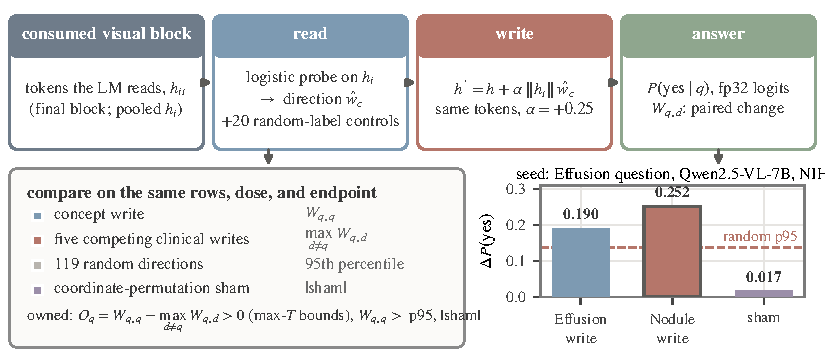
\includegraphics[width=\textwidth]{figures/fig1_framework.pdf}
    \caption{\textbf{From readable directions to semantic ownership.} A linear probe extracts named directions from the consumed visual representation and reuses them as interventions at the same block. In our patient-disjoint Qwen result, both Effusion and Nodule directions increase the Effusion answer, but Nodule is stronger. The Effusion direction remains a reproducible, non-generic writer while failing the matched clinical-family test for Effusion-specific ownership.}
    \label{fig:framework}
\end{figure*}

Our three model--concept cells on NIH ChestX-ray14 reveal two forms of reader--writer mismatch. All three cells are robustly readable, with AUROC from 0.7742 to 0.8009 and positive controlled selectivity; the paired selectivity contrasts do not resolve an ordering. The LLaVA directions do not satisfy the same generic-control criterion, whereas Qwen Effusion does so twice, including on the patient-disjoint 400-patient cohort. It is a large, reproducible, non-generic write effect whose specific Effusion attribution breaks under semantic competition because the maximum over five fixed clinical alternatives is reliably larger. We then test the implied mechanism prospectively: a full six-direction by six-question matrix finds neither a named owner nor a shared alias beyond 119 random directions, and a fresh within-patient Consolidation experiment does not close the measured input gap beyond its controls.

Our contributions are threefold. First, we formulate probe-vector interpretation as a reader--writer identification problem and introduce \emph{semantic competition}: comparing the named normal with equally constructed clinical alternatives at one consumed representation. Second, we show that robust readers need not become selective writers, and that a writer which beats random and sham controls need not be specific to its read label. Third, we follow that mismatch through two prospective mechanism gates: a complete matched clinical response surface and an input-displacement closure test. Both preserve the attribution boundary rather than recovering a concept-specific causal mechanism.

The practical principle is simple: non-semantic controls support a non-generic effect under the registered comparison, while semantic competitors and mechanism tests determine what, if anything, makes it clinically specific. Sections~\ref{sec:related}--\ref{sec:protocol} place and define these tests, Section~\ref{sec:results} follows the evidence from intervention efficacy through mechanism confirmation, and Sections~\ref{sec:discussion}--\ref{sec:conclusion} develop its implications and scope.

\section{Background and Related Work}
\label{sec:related}

\paragraph{Probing and its controls.}
Linear classifiers have long been used to track information across network depth \citep{alain2017understanding}. A probe score reflects both the representation and the learner fitted to it. This motivates matched-capacity probes and control tasks \citep{hewitt2019designing}. The probing literature distinguishes information a readout can recover from information the model uses \citep{belinkov2022probing,ravichander2021probing}. Causal erasure pursues the complementary test \citep{ravfogel2020null,elazar2021amnesic}, and a closed-form projection removes a concept from every linear reader at once \citep{belrose2023leace}. Erasure asks what breaks when a concept is deleted; the question here is whether the concept's own direction is the one that moves its answer. Our readability grade adopts the control-task idea: it measures selectivity against random-label probes of equal capacity fitted within recurring image types. Depth-wise probing of medical multimodal models has mapped classification information across towers, connectors, and language layers \citep{zhu2026lost}. Layer-wise probes of MedCLIP expose acquisition and device shortcuts \citep{pedersen2026probes}. Neither intervenes on the decoded clinical direction at the same locus.

\paragraph{Concept directions and what they inherit.}
A concept activation vector is the normal of a classifier separating concept examples from a negative set, and it grades a class by the directional derivative of the logit along that normal \citep{kim2018tcav}. We keep the direction and change the measurement: a bounded forward write at a fixed fraction of each token's norm, scored against directions built the same way for the competing concepts, rather than a gradient sensitivity read at the output. Such a normal shifts with the layer it is fitted at, entangles with correlated concepts, depends on the negative set it is fitted against, and carries where in the image the concept was read \citep{nicolson2025explaining}. Section~\ref{sec:robust-geometry} tests each: alternative constructions, a second locus, and writes concentrated on the tokens the probe reads.

\paragraph{Steering with probe normals.}
Representation engineering makes the step from reading a concept to writing it back \citep{zou2023representation}. Activation engineering changes intermediate representations at inference time and measures the resulting output changes \citep{turner2023steering,panickssery2024caa}. A probe normal is an appealing intervention because it supplies a label and a signed vector from the same representation. Separability-trained concept vectors can absorb distractor signals and diverge from the concept they are meant to model \citep{pahde2025navigating}. A classifier's weight vector is a filter, not the pattern it detects \citep{haufe2014interpretation}. Mass-mean directions steer truth judgements in language models more effectively than logistic normals \citep{marks2024geometry}. The features that identify a concept in the input are largely not the features that control the output, and selecting for output effect improves steering \citep{arad2025saes}. Benchmarks accordingly score concept detection and steering as separate axes of the same method \citep{wu2025axbench}. Random-direction and sham controls test generic sensitivity and coordinate dependence. They do not test whether an equally constructed direction with a different label would move the same answer more. Ownership adds this comparison and evaluates it in the forward path at the consumed locus, using each token's norm as the dose scale. Alignment search certifies a subspace as causal by showing that it implements an interpretable causal variable \citep{geiger2024alignments}; ownership asks a narrower question of a labelled direction: whether the label names the direction that moves its answer. Prior work replaces the separability-trained vector with a better estimator of the same concept and evaluates the replacement against the concept's own label \citep{pahde2025navigating,haufe2014interpretation,marks2024geometry}. Ownership instead fixes the estimator and varies the label: the reference family contains a direction fitted the same way for every other concept in the set, so a construction that improves estimation is scored by whether it wins that comparison. Section~\ref{sec:robust-geometry} runs five constructions and both lifts through the same test. Geometric notions such as cosine and projection depend on the inner product chosen for the representation \citep{park2024linear}, so every cosine here names its metric: cosines between directions are reported in the raw model space, and the two comparisons that carry the argument---the answer direction against the probe normal, and the expert-label refit against the report-label direction---in both the raw model space and the training covariance. It scores difference-of-means, pattern, orthogonalised, and residualised directions alongside the logistic normal (Section~\ref{sec:robust-geometry}).

\paragraph{Writing into a vision-language model.}
Image features are linearly decodable in a vision-language model's hidden layers, and targeted edits to them change downstream answers \citep{rajaram2025lineofsight}. Steering one sparse-autoencoder feature of the vision tower on an empty image and asking the language model what it sees turns the language model into a read-out of what that feature encodes \citep{ferrando2026explain}. That work steers a feature to recover its meaning; this paper starts from the meaning, fits a direction to a clinical label, and asks whether the write keeps that label's selectivity when the other findings' directions are written at the same locus, dose, and patients. Causal probing of multimodal models intervenes on the language model's residual stream with difference-in-means vectors over paired images, and reads out where entity and abstract concepts sit across depth \citep{deng2026causal}. It intervenes inside the reader and scores each concept against its own effect; the write here acts on the representation the reader consumes and scores each concept against the competing concepts' directions, which is the comparison that decides whether the label names the handle.

\section{Reading, Answering, and Writing at a Consumed Locus}
\label{sec:framework}

The evaluation asks three questions about a concept $c$ in a checkpoint $M$ on a dataset with binary labels: can $c$ be read from the visual representation the language model consumes, does $M$ answer the question about $c$, and does writing $c$'s own direction move $c$'s answer more than any alternative? Each question has a fixed estimator and a fixed decision rule; nothing is chosen after seeing the outcome.

\subsection{Consumed locus and matched read--write positions}
\label{sec:locus}

Every VLM in the grid passes an image through a vision tower and hands a specific tensor to a connector or merger that produces the language model's inputs. The \emph{primary locus} is the output of the last visual block whose output that consumer reads, restricted to the token positions the consumer actually uses (CLS or padding rows are excluded where the consumer drops them); the \emph{connector locus} is the consumer's output. Table~\ref{tab:cf-models} names the block for every family. For image $i$ and consumed token $t$ let $\hvec_{it}\in\R^D$ be the block output; mean pooling over the consumed tokens gives the read vector $\hvec_i$. The write acts on the same tokens,
\begin{equation}
\hvec'_{it}=\hvec_{it}+\alpha\,\lVert\hvec_{it}\rVert_2\,\hat\wvec_c,
\label{eq:intervention}
\end{equation}
so that the dose $\alpha$ is a fraction of each token's own norm and is comparable across families whose activation scales differ by orders of magnitude. Reading and writing therefore use the same representation and the same positions.

\subsection{Directions, controls, and the reference family}
\label{sec:directions}

A fixed seed-0 Gaussian matrix $R\in\R^{D\times512}$ projects every checkpoint to a common readout dimension; featurewise scale $\boldsymbol s$ is fitted on training rows only; logistic regression ($C=1$, 2{,}000 iterations) is fitted per concept with three seeds. The write direction lifts the positive-class coefficient $\boldsymbol\beta_c$ back to the consumed space,
\begin{equation}
\hat\wvec_c=\frac{R\left(\boldsymbol\beta_c\oslash\max(\boldsymbol s,10^{-8})\right)}{\left\lVert R\left(\boldsymbol\beta_c\oslash\max(\boldsymbol s,10^{-8})\right)\right\rVert_2}.
\label{eq:lift}
\end{equation}
Two families of controls bracket the concept direction. For reading, 20 control probes are fitted to random labels drawn within recurring image types (view, sex, and age decade on chest sets; aspect and area buckets on COCO) so that they have the same capacity and the same nuisance structure as the concept probe; selectivity is
\begin{equation}
S=\operatorname{AUROC}(y,r)-\tfrac{1}{20}\textstyle\sum_{k}\operatorname{AUROC}(y^{\mathrm{ctrl}}_k,r^{\mathrm{ctrl}}_k).
\label{eq:selectivity}
\end{equation}
For writing, the \emph{reference family} contains 119 seed-0 random unit directions, a coordinate-permutation sham of $\hat\wvec_c$ (same coordinates, scrambled arrangement), and the five directions of the other clinical concepts, all written at the same dose to the same images.

\subsection{Ownership}
\label{sec:ownership}

For question $q$ and direction $d$, $W_{q,d}$ is the paired mean change in $P(\mathrm{yes})$ of $q$ under a write along $d$, where $P(\mathrm{yes})=\sigma(\ell_{\mathrm{yes}}-\ell_{\mathrm{no}})$ at the first answer position and each log-probability is the maximum over case and leading-space variants that tokenise to one token. The $6\times6$ matrix $W$ over concept questions and concept directions is the object of interest (Figure~\ref{fig:write-matrices}). Ownership is the diagonal margin
\begin{equation}
O_q=W_{q,q}-\max_{d\neq q}W_{q,d},
\label{eq:margin}
\end{equation}
the advantage of the concept's own direction over its strongest clinical competitor on the concept's own question. A large $W_{q,q}$ shows that $d=q$ can write the answer; only $O_q>0$ shows that the label names the effective direction. Uncertainty over patients is quantified by 2{,}000 bootstrap draws of test rows with the maximum recomputed inside every draw, and the 30 contrasts $W_{q,q}-W_{q,d}$ receive simultaneous 95\% lower bounds from a centred studentised max-$T$ bootstrap (Appendix~\ref{app:simultaneous-bounds}).

\subsection{Graded outcomes}
\label{sec:grades}

\begin{itemize}[leftmargin=*,itemsep=1pt,topsep=2pt]
\item \textbf{Readable:} the one-sided 95\% lower bound of $S$ is above zero, with at least ten positives and ten negatives among the test rows.
\item \textbf{Answerable:} the one-sided 95\% lower bound of the clean-answer AUROC on the yes/no question is above $0.5$.
\item \textbf{Owned:} the write meets the \emph{steering reference}---$W_{q,q}>0$, above the 95th percentile of the 119 random writes, and above the absolute sham---and every simultaneous lower bound of $W_{q,q}-W_{q,d}$ is positive. A cell with any simultaneous upper bound below zero has a \emph{stronger competitor}; the rest are \emph{unresolved}.
\end{itemize}
Every block additionally reports the signed dose range of $O_q$ over $\alpha\in\{-0.5,\ldots,+0.5\}$, the standard deviation of $O_q$ over the three fit seeds, ownership at the connector locus, the label-shift gap (the answer change when test labels are permuted within type), and the wording (\emph{is} versus \emph{show}) and mapping (A-present versus B-present) contrasts of $O_q$ across six question templates.

\subsection{Acceptance gates}
\label{sec:gates}

Seven checks run on 16 held-out preflight rows at both loci before a block is scored (Table~\ref{tab:cf-gates}): (A) bitwise determinism on repeat; (B) identity at $\alpha=0$; (C) reach---the write changes the consumer's input and the answer logits and nothing outside the consumed tokens; (D) batch-versus-single consistency of answer logits; (E) image-free semantic mapping---the model maps ``the finding is present/absent'' statements to the intended answer token under each template; (F) throughput; (G) agreement of fp32 answer logits recomputed from the final hidden state with the model's own logits. Two measurement facts fixed the scoring design: bf16 model logits lie on a 0.125 lattice, so every answer logit is recomputed in fp32; and bf16 kernels are shape dependent, so every contrast of a question---clean, concept, five competitors, sham, and random writes---is scored in one fixed batch composition. Templates that fail (E) are \emph{ineligible} for that checkpoint and are graded as such rather than scored.

\section{Models, Datasets, and Scale}
\label{sec:setup}

\paragraph{Checkpoints.}
We evaluate 21 instruction-tuned checkpoints from nine families (Table~\ref{tab:cf-families}; full list in Table~\ref{tab:cf-models}): Qwen2.5-VL 3B/7B/32B/72B, Qwen3-VL 4B/8B/32B, InternVL3.5 8B/14B/38B, Gemma~3 4B/12B/27B, MedGemma 4B/27B, Lingshu 7B/32B, LLaVA-1.5 7B/13B, LLaVA-Med~1.5 7B, and Llama~3.2~Vision 11B. Three families are medical fine-tunes (MedGemma, Lingshu, LLaVA-Med); the rest are general-purpose. The families span five vision-tower designs and three consumer designs (token insertion after a merger, token insertion after a projector, and cross-attention), and consumed-token counts from 144 to 4{,}096 per image. Every checkpoint runs in bf16 at a pinned revision with its native processor settings and a fixed image resolution per family.

\paragraph{Datasets and concepts.}
NIH ChestX-ray14 \citep{wang2017chestxray} and CheXpert Plus provide chest radiographs with report-derived labels; we evaluate six findings on each (NIH: Effusion, Atelectasis, Pneumothorax, Cardiomegaly, Mass, Nodule; CheXpert: Effusion, Atelectasis, Pneumothorax, Cardiomegaly, Consolidation, Edema). COCO provides the natural-image control with six object categories (person, dog, car, chair, bottle, bicycle) as binary presence labels. Each dataset has one fixed cohort chosen by seeded hashes of patient (or image) identity: 20{,}000 training rows, 400 calibration rows, 600 test rows, and 16 preflight rows, patient-disjoint and shared by every checkpoint, one frontal study per patient on the chest sets.

\paragraph{Labels.} Concept labels are the report-derived labels shipped with each dataset (NIH ChestX-ray14 finding labels; the CheXpert labeler output distributed with CheXpert Plus; COCO instance annotations). A row is positive when the label is 1, negative when it is 0, and \emph{unknown} when the labeler returns uncertain or blank; unknown rows are excluded from probe fitting, selectivity, and answer AUROC, and are written and scored like every other row. Cohorts are fixed manifests drawn with recorded seeds, patient-disjoint between training and test and disjoint from every seed-study cohort; per-concept counts are in Table~\ref{tab:cf-prevalence}.

\paragraph{Questions and templates.}
Each concept is asked as a yes/no question under six templates that cross two wordings (\emph{is there} versus \emph{does the image show}) with three answer interfaces (yes/no, A-present, B-present). The primary grade uses the \emph{is}/yes-no template; the other five feed the wording and mapping contrasts. The main write dose is $\alpha=+0.25$; the dose module adds $\alpha\in\{-0.5,-0.25,-0.1,+0.1,+0.5\}$.

\paragraph{Scale.}
A block is one checkpoint on one dataset. Each chest block scores the $6\times6$ write matrix, the sham, and 119 random directions on 600 test rows (457{,}200 outcomes), plus calibration, dose, refit, connector-locus, and template modules; COCO blocks run the full module set and CheXpert blocks the write matrix and calibration. The campaign comprises 61 blocks, 342 scored concept cells, about 30 million scored answers, and roughly 3{,}000 A100-hours. Nineteen checkpoints are complete on all three datasets; Llama~3.2~Vision 11B is graded on its eligible templates; Qwen2.5-VL-72B is run on NIH only, and no checkpoint above 72B is run (Appendix~\ref{app:campaign}).

\paragraph{Registration.} The protocol was frozen before any block of the grid was scored: the loci, the projection and probe settings, the dose, the reference family, the six templates, the module set, the seven gates, and the three decision rules are those of the registered protocol file and its code commit, and the seed study's crossover and confirmation analyses were registered before they were run (Appendix~\ref{app:seed}). Everything reported per block is produced by one analysis pass from the packaged outcomes; the leaderboard, the write-flow share, and the per-image examples are descriptive summaries of those outputs added after the grid was complete.

\paragraph{Artifact.} The release contains the evaluation code and adapters, the registered protocol file, the cohort manifests with their seeds, the fitted directions, the per-image outcomes of every module (write, dose, refit, locus, and template rows), every block's scorecard and coverage file, and the rendered prompts; a new checkpoint is added with one adapter that names its consumed block and passes the gates.

\section{Results}
\label{sec:results}

\subsection{Reading is not writing}
\label{sec:headline}

Table~\ref{tab:cf-main} reports scores for every checkpoint on every dataset. Figure~\ref{fig:overview} shows every concept cell across the three grades. Both chest datasets follow the same pattern. On the calibration cohort, clinical concepts are readable in \cfChestReadable{} of \cfChestReadableN{} cells (\cfChestReadablePct\%): probe selectivity exceeds matched random-label controls by $0.1$--$0.3$ for most findings in most families. The models also answer on this cohort: \cfChestAnswerable{} of the \cfChestAnswerableN{} cells with a scored write matrix (\cfChestAnswerablePct\%) have a clean-answer AUROC lower bound above chance on the same 400 rows. Of these answerable cells, \cfReadAns{} are also readable. Yet only \cfChestOwned{} cells (\cfChestOwnedPct\%) are owned. In \cfChestCompetitor{} cells (\cfChestCompetitorPct\%), the verdict is \emph{stronger competitor}: a direction fitted for another finding moves the concept's answer more than the concept's own direction does. Readability and answerability do not suffice for writing: only \cfReadAnsOwned{} of the \cfReadAns{} readable and answerable cells are owned (\cfReadAnsOwnedPct\%), compared with \cfRestOwned{} of the remaining \cfRestN{} (\cfRestOwnedPct\%).

Table~\ref{tab:cf-contingency} groups chest cells by steering-reference status and clinical comparison verdict. To meet the steering reference, the concept's own write must raise its answer above both the 95th percentile of the random writes and the absolute sham. Of the \cfChestAnswerableN{} chest cells, \cfChestRefMet{} meet this reference. Among these \cfChestRefMet{} cells, \cfChestOwned{} are owned, \cfChestRefStrong{} have a stronger competitor, and \cfChestRefUnres{} are unresolved. The remaining \cfChestRefBelow{} cells fall below the steering reference and account for \cfChestBelowStrong{} of the \cfChestCompetitor{} stronger-competitor verdicts (\cfChestBelowStrongPct\%). In these cells, the concept's own write fails to clear the random and sham references. A direction fitted for another finding moves the concept's answer more. Readable and answerable cells show the same pattern. Of the \cfReadAns{} readable and answerable cells, \cfReadAnsRefMet{} meet the steering reference. Among these, \cfReadAnsOwned{} are owned, \cfReadAnsRefStrong{} have a stronger competitor, and \cfReadAnsRefUnres{} are unresolved. Of the \cfReadAnsCompetitor{} stronger-competitor verdicts for readable and answerable cells, \cfReadAnsBelowStrong{} occur in the \cfReadAnsRefBelow{} cells below the reference. On COCO, \cfCocoRefMet{} of \cfCocoOwnedN{} cells meet the steering reference. Of these, \cfCocoOwned{} are owned. Of the \cfCocoCompetitor{} stronger-competitor verdicts, \cfCocoBelowStrong{} occur below the reference.

\begin{table}[t]
\centering
\scriptsize
\setlength{\tabcolsep}{2pt}
\renewcommand{\arraystretch}{1.08}
% Morandi tints for the cf-transfer tables (muted, low saturation); darker = larger value
\definecolor{cfSage1}{HTML}{EEF1EA}
\definecolor{cfSage2}{HTML}{D9E1D2}
\definecolor{cfSage3}{HTML}{C1CDB8}
\definecolor{cfSage4}{HTML}{A6B79C}
\definecolor{cfSlate1}{HTML}{ECEFF2}
\definecolor{cfSlate2}{HTML}{D3DAE2}
\definecolor{cfSlate3}{HTML}{B7C3D0}
\definecolor{cfSlate4}{HTML}{98A8B9}
\definecolor{cfTerra1}{HTML}{F5ECE9}
\definecolor{cfTerra2}{HTML}{E9D3CC}
\definecolor{cfTerra3}{HTML}{DAB5AA}
\definecolor{cfTerra4}{HTML}{C9968A}
\definecolor{cfOat1}{HTML}{F4EFE6}
\definecolor{cfOat2}{HTML}{E8DDC8}
\definecolor{cfGrey}{HTML}{E4E1DC}

\caption{\textbf{Reading, answering, and writing per checkpoint.} Per dataset: mean probe selectivity (\textsc{Read}), clean-answer AUROC (\textsc{Ans}), and ownership (\textsc{Own}), superscripted with the graded concepts of six, then the owned share of clinical and COCO cells and their ratio. Grey marks an ineligible template (inel.), an incomplete write matrix (inc.); ``--'' is a block not run.}
\label{tab:cf-main}
\begin{tabular}{l@{\hspace{3pt}}ccc@{\hspace{4pt}}ccc@{\hspace{4pt}}ccc@{\hspace{4pt}}ccc}
\toprule
& \multicolumn{3}{c}{NIH ChestX-ray14} & \multicolumn{3}{c}{CheXpert Plus} & \multicolumn{3}{c}{COCO (control)} & \multicolumn{3}{c}{Owned share} \\
\cmidrule(lr){2-4}\cmidrule(lr){5-7}\cmidrule(lr){8-10}\cmidrule(lr){11-13}
Checkpoint & \textsc{Read} & \textsc{Ans} & \textsc{Own} & \textsc{Read} & \textsc{Ans} & \textsc{Own} & \textsc{Read} & \textsc{Ans} & \textsc{Own} & clin. & COCO & ratio \\
\midrule
Lingshu 32B & \cellcolor{cfSage2}0.08$^{3}$ & \cellcolor{cfSage3}0.78$^{6}$ & \cellcolor{cfTerra2}-0.02$^{2}$ & \cellcolor{cfSage4}0.20$^{4}$ & \cellcolor{cfSage3}0.87$^{5}$ & \cellcolor{cfSlate2}+0.04$^{5}$ & \cellcolor{cfSage1}0.03$^{1}$ & \cellcolor{cfSage4}0.95$^{5}$ & \cellcolor{cfSlate4}+0.28$^{6}$ & \cellcolor{cfSlate4}58\% & \cellcolor{cfSlate4}100\% & 58\% \\
CheXagent-2-3B & \cellcolor{cfSage3}0.13$^{5}$ & \cellcolor{cfSage3}0.86$^{6}$ & \cellcolor{cfSlate1}+0.00$^{2}$ & \cellcolor{cfSage4}0.21$^{5}$ & \cellcolor{cfSage4}0.95$^{5}$ & \cellcolor{cfSlate1}+0.01$^{4}$ & \cellcolor{cfSage3}0.13$^{4}$ & \cellcolor{cfSage3}0.81$^{5}$ & \cellcolor{cfSlate2}+0.03$^{2}$ & \cellcolor{cfSlate4}50\% & \cellcolor{cfSlate2}33\% & 150\% \\
Qwen2.5-VL-72B & \cellcolor{cfSage2}0.07$^{2}$ & \cellcolor{cfSage2}0.62$^{4}$ & \cellcolor{cfTerra2}-0.03$^{3}$ & \cellcolor{cfSage3}0.20$^{4}$ & \cellcolor{cfSage2}0.71$^{4}$ & \cellcolor{cfTerra2}-0.09$^{1}$ & \cellcolor{cfSage1}0.01$^{1}$ & \cellcolor{cfSage4}0.99$^{5}$ & \cellcolor{cfSlate4}+0.66$^{6}$ & \cellcolor{cfSlate3}33\% & \cellcolor{cfSlate4}100\% & 33\% \\
Lingshu 7B & \cellcolor{cfSage2}0.08$^{3}$ & \cellcolor{cfSage3}0.76$^{6}$ & \cellcolor{cfSlate2}+0.02$^{1}$ & \cellcolor{cfSage4}0.21$^{4}$ & \cellcolor{cfSage3}0.86$^{5}$ & \cellcolor{cfSlate2}+0.04$^{3}$ & \cellcolor{cfSage1}0.02$^{1}$ & \cellcolor{cfSage4}0.97$^{5}$ & \cellcolor{cfSlate4}+0.68$^{6}$ & \cellcolor{cfSlate3}33\% & \cellcolor{cfSlate4}100\% & 33\% \\
Qwen3-VL-4B & \cellcolor{cfSage2}0.08$^{3}$ & \cellcolor{cfSage2}0.71$^{6}$ & \cellcolor{cfTerra3}-0.11$^{0}$ & \cellcolor{cfSage4}0.20$^{4}$ & \cellcolor{cfSage2}0.74$^{4}$ & \cellcolor{cfTerra1}-0.01$^{2}$ & \cellcolor{cfSage1}0.04$^{4}$ & \cellcolor{cfSage4}0.99$^{5}$ & \cellcolor{cfSlate4}+0.34$^{6}$ & \cellcolor{cfSlate3}17\% & \cellcolor{cfSlate4}100\% & 17\% \\
Qwen3-VL-32B & \cellcolor{cfSage2}0.10$^{2}$ & \cellcolor{cfSage2}0.70$^{6}$ & \cellcolor{cfTerra2}-0.02$^{1}$ & \cellcolor{cfSage3}0.17$^{5}$ & \cellcolor{cfSage3}0.82$^{5}$ & \cellcolor{cfTerra2}-0.02$^{1}$ & \cellcolor{cfSage2}0.05$^{4}$ & \cellcolor{cfSage4}0.99$^{5}$ & \cellcolor{cfSlate3}+0.15$^{6}$ & \cellcolor{cfSlate3}17\% & \cellcolor{cfSlate4}100\% & 17\% \\
InternVL3.5-38B & \cellcolor{cfSage2}0.10$^{5}$ & \cellcolor{cfSage3}0.78$^{6}$ & \cellcolor{cfTerra1}-0.00$^{0}$ & \cellcolor{cfSage3}0.17$^{4}$ & \cellcolor{cfSage3}0.86$^{5}$ & \cellcolor{cfTerra1}-0.00$^{2}$ & \cellcolor{cfSage2}0.08$^{4}$ & \cellcolor{cfSage4}0.99$^{5}$ & \cellcolor{cfSlate1}+0.01$^{6}$ & \cellcolor{cfSlate3}17\% & \cellcolor{cfSlate4}100\% & 17\% \\
Gemma 3 12B & \cellcolor{cfSage2}0.07$^{2}$ & \cellcolor{cfSage2}0.62$^{5}$ & \cellcolor{cfTerra4}-0.37$^{1}$ & \cellcolor{cfSage3}0.18$^{4}$ & \cellcolor{cfSage1}0.52$^{0}$ & \cellcolor{cfTerra4}-0.38$^{1}$ & \cellcolor{cfSage2}0.07$^{5}$ & \cellcolor{cfSage4}0.95$^{5}$ & \cellcolor{cfSlate4}+0.44$^{6}$ & \cellcolor{cfSlate3}17\% & \cellcolor{cfSlate4}100\% & 17\% \\
MedGemma 4B & \cellcolor{cfSage3}0.12$^{3}$ & \cellcolor{cfSage3}0.80$^{6}$ & \cellcolor{cfTerra3}-0.13$^{0}$ & \cellcolor{cfSage4}0.21$^{4}$ & \cellcolor{cfSage3}0.87$^{5}$ & \cellcolor{cfTerra3}-0.16$^{2}$ & \cellcolor{cfSage2}0.06$^{4}$ & \cellcolor{cfSage4}0.94$^{5}$ & \cellcolor{cfSlate3}+0.23$^{6}$ & \cellcolor{cfSlate3}17\% & \cellcolor{cfSlate4}100\% & 17\% \\
InternVL3.5-14B & \cellcolor{cfSage2}0.07$^{4}$ & \cellcolor{cfSage2}0.73$^{6}$ & \cellcolor{cfTerra1}-0.00$^{1}$ & \cellcolor{cfSage3}0.16$^{4}$ & \cellcolor{cfSage3}0.87$^{5}$ & \cellcolor{cfSlate1}+0.00$^{1}$ & \cellcolor{cfSage3}0.12$^{4}$ & \cellcolor{cfSage4}0.98$^{5}$ & \cellcolor{cfSlate1}+0.02$^{5}$ & \cellcolor{cfSlate3}17\% & \cellcolor{cfSlate3}83\% & 20\% \\
Qwen2.5-VL-32B & \cellcolor{cfSage2}0.09$^{3}$ & \cellcolor{cfSage2}0.63$^{4}$ & \cellcolor{cfTerra2}-0.06$^{1}$ & \cellcolor{cfSage3}0.16$^{4}$ & \cellcolor{cfSage2}0.70$^{4}$ & \cellcolor{cfTerra3}-0.11$^{0}$ & \cellcolor{cfSage1}0.02$^{1}$ & \cellcolor{cfSage4}0.99$^{5}$ & \cellcolor{cfSlate4}+0.38$^{6}$ & \cellcolor{cfSlate2}8\% & \cellcolor{cfSlate4}100\% & 8\% \\
InternVL3.5-8B & \cellcolor{cfSage2}0.06$^{2}$ & \cellcolor{cfSage2}0.73$^{6}$ & \cellcolor{cfTerra1}-0.01$^{0}$ & \cellcolor{cfSage3}0.19$^{4}$ & \cellcolor{cfSage3}0.86$^{5}$ & \cellcolor{cfTerra1}-0.00$^{1}$ & \cellcolor{cfSage2}0.12$^{5}$ & \cellcolor{cfSage4}0.98$^{5}$ & \cellcolor{cfSlate2}+0.03$^{6}$ & \cellcolor{cfSlate2}8\% & \cellcolor{cfSlate4}100\% & 8\% \\
HuatuoGPT-Vision-7B & \cellcolor{cfSage2}0.08$^{3}$ & \cellcolor{cfSage2}0.71$^{6}$ & \cellcolor{cfTerra2}-0.03$^{1}$ & \cellcolor{cfSage3}0.19$^{4}$ & \cellcolor{cfSage3}0.78$^{4}$ & \cellcolor{cfTerra1}-0.01$^{0}$ & \cellcolor{cfSage2}0.07$^{4}$ & \cellcolor{cfSage4}0.99$^{5}$ & \cellcolor{cfSlate1}+0.01$^{4}$ & \cellcolor{cfSlate2}8\% & \cellcolor{cfSlate3}67\% & 12\% \\
LLaVA-Med 1.5 7B & \cellcolor{cfSage2}0.08$^{3}$ & \cellcolor{cfSage1}0.53$^{0}$ & \cellcolor{cfTerra1}-0.01$^{0}$ & \cellcolor{cfSage3}0.19$^{4}$ & \cellcolor{cfSage1}0.59$^{2}$ & \cellcolor{cfTerra1}-0.01$^{1}$ & \cellcolor{cfSage2}0.07$^{4}$ & \cellcolor{cfSage3}0.76$^{5}$ & \cellcolor{cfSlate1}+0.00$^{1}$ & \cellcolor{cfSlate2}8\% & \cellcolor{cfSlate2}17\% & 50\% \\
CheXagent-8B & \cellcolor{cfSage3}0.16$^{5}$ & \cellcolor{cfSage2}0.73$^{6}$ & \cellcolor{cfTerra1}-0.00$^{0}$ & \cellcolor{cfSage4}0.23$^{5}$ & \cellcolor{cfSage3}0.88$^{5}$ & \cellcolor{cfTerra1}-0.02$^{1}$ & \cellcolor{cfSage2}0.05$^{3}$ & \cellcolor{cfSage1}0.52$^{1}$ & \cellcolor{cfTerra2}-0.03$^{0}$ & \cellcolor{cfSlate2}8\% & \cellcolor{cfSlate1}0\% & -- \\
Qwen2.5-VL-3B & \cellcolor{cfSage2}0.07$^{2}$ & \cellcolor{cfSage1}0.58$^{2}$ & \cellcolor{cfTerra2}-0.08$^{0}$ & \cellcolor{cfSage3}0.17$^{4}$ & \cellcolor{cfSage1}0.57$^{2}$ & \cellcolor{cfTerra2}-0.07$^{0}$ & \cellcolor{cfSage1}0.05$^{4}$ & \cellcolor{cfSage4}0.97$^{5}$ & \cellcolor{cfSlate4}+0.52$^{6}$ & \cellcolor{cfSlate1}0\% & \cellcolor{cfSlate4}100\% & 0\% \\
Qwen2.5-VL-7B & \cellcolor{cfSage2}0.08$^{3}$ & \cellcolor{cfSage2}0.62$^{3}$ & \cellcolor{cfTerra3}-0.14$^{0}$ & \cellcolor{cfSage3}0.20$^{4}$ & \cellcolor{cfSage2}0.65$^{2}$ & \cellcolor{cfTerra2}-0.08$^{0}$ & \cellcolor{cfSage1}0.02$^{1}$ & \cellcolor{cfSage4}0.98$^{5}$ & \cellcolor{cfSlate4}+0.67$^{6}$ & \cellcolor{cfSlate1}0\% & \cellcolor{cfSlate4}100\% & 0\% \\
Qwen3-VL-8B & \cellcolor{cfSage2}0.10$^{4}$ & \cellcolor{cfSage2}0.69$^{6}$ & \cellcolor{cfTerra1}-0.01$^{0}$ & \cellcolor{cfSage3}0.17$^{4}$ & \cellcolor{cfSage2}0.75$^{4}$ & \cellcolor{cfTerra2}-0.04$^{0}$ & \cellcolor{cfSage1}0.04$^{3}$ & \cellcolor{cfSage4}0.99$^{5}$ & \cellcolor{cfSlate4}+0.58$^{6}$ & \cellcolor{cfSlate1}0\% & \cellcolor{cfSlate4}100\% & 0\% \\
Gemma 3 27B & \cellcolor{cfSage2}0.07$^{2}$ & \cellcolor{cfSage2}0.60$^{3}$ & \cellcolor{cfTerra2}-0.03$^{0}$ & \cellcolor{cfSage3}0.18$^{4}$ & \cellcolor{cfSage1}0.55$^{2}$ & \cellcolor{cfTerra1}-0.01$^{0}$ & \cellcolor{cfSage2}0.07$^{5}$ & \cellcolor{cfSage4}0.96$^{5}$ & \cellcolor{cfSlate4}+0.31$^{6}$ & \cellcolor{cfSlate1}0\% & \cellcolor{cfSlate4}100\% & 0\% \\
Gemma 3 4B & \cellcolor{cfSage2}0.07$^{2}$ & \cellcolor{cfSage1}0.56$^{2}$ & \cellcolor{cfTerra3}-0.11$^{0}$ & \cellcolor{cfSage3}0.18$^{4}$ & \cellcolor{cfSage1}0.53$^{1}$ & \cellcolor{cfTerra4}-0.27$^{0}$ & \cellcolor{cfSage2}0.07$^{5}$ & \cellcolor{cfSage4}0.94$^{5}$ & \cellcolor{cfSlate3}+0.24$^{5}$ & \cellcolor{cfSlate1}0\% & \cellcolor{cfSlate3}83\% & 0\% \\
LLaVA-1.5-7B & \cellcolor{cfSage2}0.08$^{2}$ & \cellcolor{cfSage1}0.51$^{0}$ & \cellcolor{cfTerra2}-0.04$^{0}$ & \cellcolor{cfSage3}0.17$^{4}$ & \cellcolor{cfSage1}0.52$^{0}$ & \cellcolor{cfTerra2}-0.03$^{0}$ & \cellcolor{cfSage4}0.28$^{5}$ & \cellcolor{cfSage4}0.97$^{5}$ & \cellcolor{cfSlate2}+0.03$^{5}$ & \cellcolor{cfSlate1}0\% & \cellcolor{cfSlate3}83\% & 0\% \\
MedGemma 27B & \cellcolor{cfSage3}0.12$^{3}$ & \cellcolor{cfSage3}0.80$^{6}$ & \cellcolor{cfTerra3}-0.14$^{0}$ & \cellcolor{cfSage4}0.21$^{4}$ & \cellcolor{cfSage3}0.87$^{5}$ & \cellcolor{cfTerra2}-0.06$^{0}$ & \cellcolor{cfSage2}0.06$^{4}$ & \cellcolor{cfSage4}0.97$^{5}$ & \cellcolor{cfSlate3}+0.12$^{4}$ & \cellcolor{cfSlate1}0\% & \cellcolor{cfSlate3}67\% & 0\% \\
LLaVA-1.5-13B & \cellcolor{cfSage2}0.08$^{2}$ & \cellcolor{cfSage1}0.53$^{0}$ & \cellcolor{cfTerra2}-0.02$^{0}$ & \cellcolor{cfSage3}0.17$^{4}$ & \cellcolor{cfSage1}0.51$^{1}$ & \cellcolor{cfTerra1}-0.01$^{0}$ & \cellcolor{cfSage4}0.28$^{5}$ & \cellcolor{cfSage4}0.96$^{5}$ & \cellcolor{cfSlate2}+0.02$^{2}$ & \cellcolor{cfSlate1}0\% & \cellcolor{cfSlate2}33\% & 0\% \\
Llama 3.2 Vision 11B & \cellcolor{cfSage2}0.08$^{2}$ & \cellcolor{cfSage2}0.65$^{4}$ & \cellcolor{cfTerra2}-0.03$^{0}$ & \cellcolor{cfSage3}0.16$^{4}$ & \cellcolor{cfSage2}0.73$^{4}$ & \cellcolor{cfTerra2}-0.04$^{0}$ & \cellcolor{cfSage3}0.12$^{5}$ & \cellcolor{cfSage4}0.95$^{5}$ & \cellcolor{cfTerra1}-0.01$^{1}$ & \cellcolor{cfSlate1}0\% & \cellcolor{cfSlate2}17\% & 0\% \\
LLaVA-Rad-7B & \cellcolor{cfSage3}0.15$^{4}$ & \cellcolor{cfSage2}0.71$^{5}$ & \cellcolor{cfTerra1}-0.01$^{0}$ & \cellcolor{cfSage4}0.27$^{5}$ & \cellcolor{cfSage3}0.87$^{5}$ & \cellcolor{cfTerra1}-0.02$^{0}$ & \cellcolor{cfSage3}0.12$^{4}$ & \cellcolor{cfSage1}0.50$^{0}$ & \cellcolor{cfTerra2}-0.03$^{0}$ & \cellcolor{cfSlate1}0\% & \cellcolor{cfSlate1}0\% & -- \\
\midrule
\textbf{All cells} & 0.09 & 0.68 & -0.06 & 0.19 & 0.74 & -0.05 & 0.08 & 0.92 & +0.23 & 13\% & 75\% & 17\% \\
\quad count / cells & 74/150 & 110/150 & 13/150 & 104/150 & 89/150 & 25/150 & 90/150 & 116/150 & 113/150 & & & \\
\bottomrule
\end{tabular}
\end{table}


\begin{table}[t]
\centering
\small
\setlength{\tabcolsep}{4pt}
\caption{\textbf{Steering reference against verdict.} Primary write-matrix cells of the included blocks, cross-classified by the steering reference and by the simultaneous-bound verdict against the five other clinical directions.}
\label{tab:cf-contingency}
\begin{tabular}{llrrrr}
\toprule
Cells & Steering reference & advantage & stronger competitor & unresolved & total \\
\midrule
Chest, all cells & met & 29 & 8 & 7 & 44 \\
 & not met & 19 & 155 & 28 & 202 \\
Chest, readable and answerable & met & 21 & 4 & 3 & 28 \\
 & not met & 9 & 52 & 12 & 73 \\
COCO, all cells & met & 101 & 0 & 2 & 103 \\
 & not met & 6 & 10 & 1 & 17 \\
\bottomrule
\end{tabular}
\end{table}


\begin{figure}[t]
    \centering
    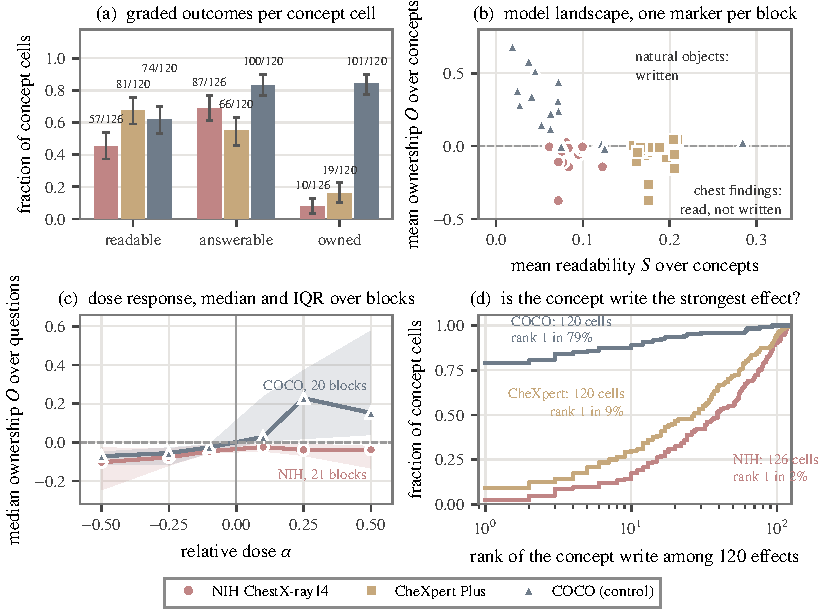
\includegraphics[width=\textwidth]{figures/fig2_overview.pdf}
    \caption{\textbf{Reading, answering, and writing across the grid.} (a) Readable, answerable, and owned cells per dataset (counts on the bars; descriptive bootstrap intervals over cells). (b) Mean readability against mean ownership per checkpoint. (c) Median ownership against the relative dose (median and interquartile band across the \cfDoseBlocksNih{} NIH and \cfDoseBlocksCoco{} COCO blocks with the dose module). (d) Rank of the concept write among the 120 compared effects.}
    \label{fig:overview}
\end{figure}

\subsection{The seed finding replicates on new patients}
\label{sec:seed}

We build on a two-model NIH study of Qwen2.5-VL-7B and LLaVA-1.5-7B (Appendix~\ref{app:seed}). In a 600-image cohort disjoint from every earlier cohort, we reproduce its central result (Table~\ref{tab:cf-seed}). The Effusion write raises the Effusion answer by $\cfSeedWEff$. This increase exceeds the random 95th percentile ($\cfSeedEffRandP$) and sham ($\cfSeedEffSham$). It ranks second among the 120 compared effects. Yet the Nodule direction raises the Effusion answer by $\cfSeedWNodule$. Effusion ownership is $O_{\mathrm{Effusion}}=\cfSeedEffO$ (95\% CI $[\cfSeedEffOLo,\cfSeedEffOHi]$), matching the original $-0.057$ $[-0.069,-0.045]$. We also reproduce the prompt dependence of Mass. Effusion and Cardiomegaly are the most readable chest concepts, with mean selectivity $\cfSelEffusion$ and $\cfSelCardiomegaly$ over \cfChestProbeBlocks{} chest blocks. Effusion is owned in \cfEffusionOwnedBlocks{} of \cfChestBlocks{} chest blocks. In \cfEffusionOwnedSmall{} of these blocks, $O_{\mathrm{Effusion}}\leq0.03$.

\subsection{The attribution deficit across the grid}
\label{sec:deficit}

On the chest sets, ownership is the rarest and least stable of the three grades. An effect floor of $0.05$ on both $W_{q,q}$ and $O_q$ retains \cfChestFloored{} of the \cfChestOwned{} owned chest cells (\cfChestFlooredPct\% of \cfChestAnswerableN{}), compared with \cfCocoFloored{} of the \cfCocoOwned{} owned COCO cells (\cfCocoFlooredPct\%). Ownership survives both probe refits on resampled patients in \cfRefitGradeStableNih{} of the \cfRefitGradeOwnedNih{} owned NIH cells, compared with \cfRefitGradeStableCoco{} of \cfRefitGradeOwnedCoco{} on COCO (Table~\ref{tab:cf-refit}). Clinical writes are not selective on the chest sets. To compute the write-flow share, we take the positive part of every entry of $W$ and average over checkpoints. We then divide the sum of the six own-question entries by the total. The written concept's own question receives \cfOwnShareNih\% of the positive answer change on NIH and \cfOwnShareChex\% on CheXpert, compared with \cfOwnShareCoco\% on COCO (Figure~\ref{fig:cf-w-structure}). This pattern is the attribution deficit. The model makes the concept readable to a probe. The probe's direction is not a handle on the concept. Writing it back moves other findings' answers as much as the concept's own.

Figure~\ref{fig:example} shows this pattern in individual images. On a chest radiograph, the Effusion and Nodule writes raise the same answers. The competing write raises the Effusion answer more than the Effusion write does. On a natural image, the dog write moves only the dog answer. The write matrix reveals two components of the deficit (Figure~\ref{fig:write-matrices}, Table~\ref{tab:cf-controls}). First, concept writes in the chest datasets have little effect on their own answers. The median $W_{q,q}$ is $\cfMedianWqqNih$ on NIH and $\cfMedianWqqChex$ on CheXpert, compared with $\cfMedianWqqCoco$ on COCO. Second, competing directions share the effect whenever a chest write moves an answer (Table~\ref{tab:cf-contingency}). Across the grid, the Atelectasis, Effusion, and Consolidation directions raise each other's answers by similar amounts. On COCO, the diagonal entry of $W$ dominates its row. On NIH and CheXpert, the row is flat or peaks off the diagonal. At every Qwen2.5-VL size, a competing direction raises the Effusion answer more than the Effusion direction does: Cardiomegaly at 3B, Nodule at 7B and 32B, and Atelectasis at 72B.

\subsection{The write mechanism is intact on natural objects}
\label{sec:coco}

On COCO, the same procedure yields the opposite result (Table~\ref{tab:cf-main}, right block). Object ownership holds in \cfCocoOwned{} of \cfCocoOwnedN{} cells (\cfCocoOwnedPct\%). Ownership margins span $\cfCocoMarginMin$--$\cfCocoMarginMax$ in the Qwen, Lingshu, and Gemma families. \cfCocoRefMet{} cells meet the steering reference. Only \cfCocoCompetitor{} cells have a stronger competitor. \cfCocoBlocksFourPlus{} of the \cfCocoBlocks{} checkpoints with a COCO block own at least four of the six objects. Dose response tracks the write. On COCO, median ownership across questions and blocks rises from $\cfDoseCocoLow$ at $\alpha=-0.1$ to $\cfDoseCocoPeak$ at $\alpha=+0.25$. Median ownership remains positive at $\alpha=+0.5$ ($\cfDoseCocoHalf$). On NIH, median ownership stays between $\cfDoseNihMin$ and $\cfDoseNihMax$ at every dose (Figure~\ref{fig:overview}c). The write, direction construction, reference family, and decision rules thus work as intended.

Task difficulty does not explain the contrast. Six small or fine-grained COCO categories---handbag, book, backpack, traffic light, knife, and cell phone---chosen by a rule fixed before the grid was built are fitted, written and graded exactly like the six easy objects in the same blocks and rows. They are owned in \cfFgFineOwned{} of \cfFgFineCells{} cells, a rate of \cfFgFineRate{} against \cfFgEasyRate{} for the easy six (\cfFgEasyOwned{} of \cfFgEasyCells{}). Median clean-answer AUROC is \cfFgFineAuroc{} against \cfFgEasyAuroc{}. Median probe selectivity is \cfFgFineSel{} against \cfFgEasySel{} (Table~\ref{tab:cf-fgobj}). Object size and fine-grainedness do not reduce ownership. Matching chest cells to natural-image cells of comparable difficulty preserves the contrast. We pair each chest cell with every natural-image cell whose matching variables lie within \cfFgWindow{} of the chest cell's values. We calculate ownership rates over the surviving pairs. Matching on probe selectivity alone pairs all \cfFgMatchSelN{} of \cfFgMatchSelCells{} chest cells and leaves ownership rates at \cfFgMatchSelChest{} against \cfFgMatchSelNat{} (difference $\cfFgMatchSelDiff$, 95\% interval $[\cfFgMatchSelLo,\cfFgMatchSelHi]$ over a cluster bootstrap whose unit is the model). Matching on clean-answer AUROC alone pairs \cfFgMatchAnsN{} and leaves \cfFgMatchAnsChest{} against \cfFgMatchAnsNat{}. Matching on both pairs \cfFgMatchBothN{} and leaves \cfFgMatchBothChest{} against \cfFgMatchBothNat{}. Probe quality does not separate the two sides: every chest cell finds a natural-image partner at its own selectivity, and ownership rates remain unchanged. Answer accuracy is the axis that excludes chest cells from the comparison. The chest cells that survive this matching already have accurate clean answers. The deficit is specific to clinical concepts rather than to task difficulty.

\begin{figure}[t]
    \centering
    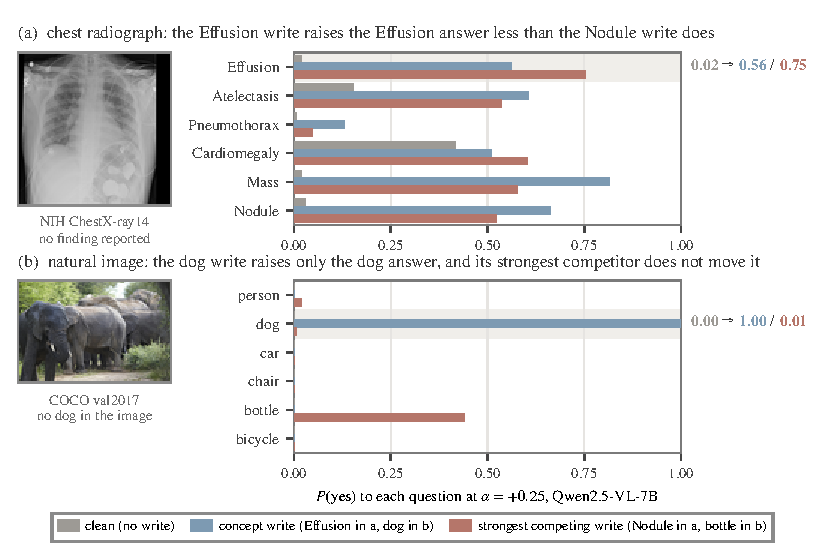
\includegraphics[width=\textwidth]{figures/fig3_example.pdf}
    \caption{\textbf{Two images, six questions, three writes.} $P(\mathrm{yes})$ per question for one NIH radiograph (top) and one COCO image (bottom) under the clean input, the concept write, and the strongest competing write, at $\alpha=+0.25$ in Qwen2.5-VL-7B. The Effusion write raises the Effusion answer from $0.02$ to $0.56$ and the Nodule write to $0.75$; the dog write moves the dog answer from $0.00$ to $1.00$ and nothing else.}
    \label{fig:example}
\end{figure}

\begin{figure}[t]
    \centering
    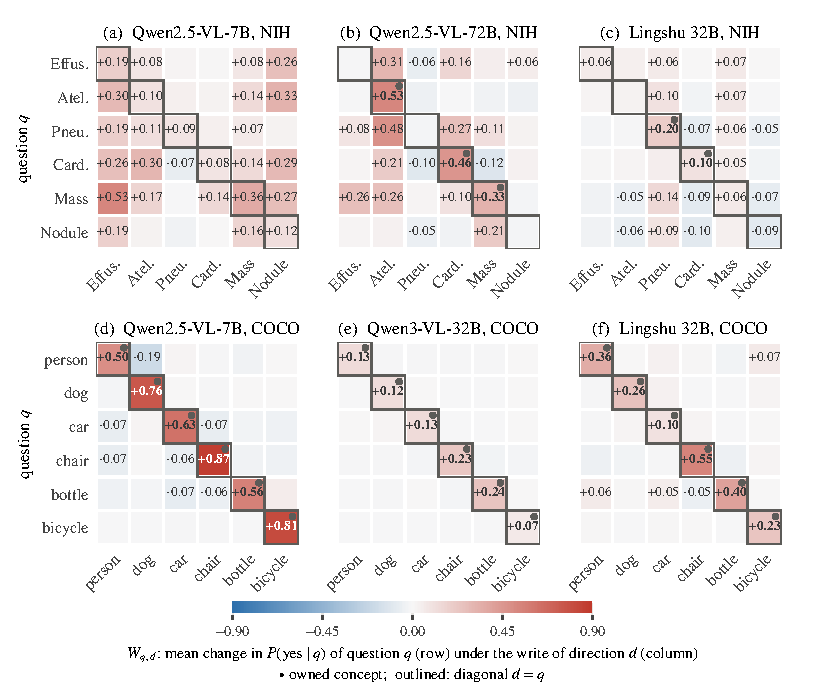
\includegraphics[width=\textwidth]{figures/fig4_write_matrices.pdf}
    \caption{\textbf{Write matrices.} $W_{q,d}$, the mean change in $P(\mathrm{yes})$ of question $q$ (rows) under the write of direction $d$ (columns), for three checkpoints on NIH (top) and three on COCO (bottom); the diagonal is outlined and owned concepts carry a dot. On COCO the diagonal dominates its row; on NIH the rows are flat or peak off the diagonal.}
    \label{fig:write-matrices}
\end{figure}

\subsection{Ownership belongs to the representation and the reader together}
\label{sec:reader}

Gemma~3 shares one SigLIP tower across its 4B, 12B, and 27B checkpoints. MedGemma shares one MedSigLIP tower across 4B and 27B. LLaVA-1.5 shares one CLIP tower across 7B and 13B. We intervene primarily at the tower's final block. This design changes the reader while holding the representation and write fixed. Within each family, pooled features, fitted probes, and lifted write vectors are identical across sizes. The connector and language model that read them differ. Features and write vectors are bit-identical for Gemma~3 4B and 12B and for LLaVA-1.5, and equal within one bf16 rounding step for Gemma~3 27B and MedGemma 27B. Raw model-space cosines between corresponding write vectors exceed $\cfPairsTowerCosMin$ for every concept and pair. Readability is identical across sizes by construction. The connector and language model produce every difference in Figure~\ref{fig:readers} by reading the same written representation differently. The median paired difference is \cfPairsRatioMin{}--\cfPairsRatioMax{} times the refit standard deviation. It exceeds that standard deviation in \cfPairsRatioAboveOne{} of the \cfPairsRatioN{} pairs with a refit estimate (Table~\ref{tab:cf-pairs}). On NIH Effusion, the identical write on the same 600 patients yields an $O_q$ difference of $\cfPairDeltaEffFourTwelve$ $[\cfPairDeltaEffFourTwelveLo,\cfPairDeltaEffFourTwelveHi]$ between Gemma~3 4B and 12B. The difference between 12B and 27B is $\cfPairDeltaEffTwelveTwentySeven$ $[\cfPairDeltaEffTwelveTwentySevenLo,\cfPairDeltaEffTwelveTwentySevenHi]$. In \cfPairsFiveOrSix{} of the \cfPairsN{} shared-tower pair--dataset combinations, the paired patient-bootstrap interval for $\Delta O_q$ excludes zero for five or six of the six concepts. The median $|\Delta O_q|$ is \cfPairsRatioMin{}--\cfPairsRatioMax{} times the families' refit standard deviation (up to \cfPairsRatioSingleMax{} times for single concepts). In 12B, competing directions own the chest answers outright ($O_{\mathrm{Effusion}}=\cfOGemmaTwelveEff$ on both chest sets, $O_{\mathrm{Mass}}=\cfOGemmaTwelveMass$, $O_{\mathrm{Pneumothorax}}=\cfOGemmaTwelvePneu$). In 27B, no direction moves these answers ($\cfOGemmaTwentySevenEff$, $\cfOGemmaTwentySevenMass$, $\cfOGemmaTwentySevenPneu$). In 4B, the clean answer is yes on \cfGemmaFourYesMin--\cfGemmaFourYesMax\% of chest rows. Every own write lowers its answer's logit margin by more than any competing write raises it ($O^m_q$ from $\cfPairsGemmaFourOmNear$ to $\cfPairsGemmaFourOmFar$, all intervals below zero). MedGemma 4B and 27B differ in the same way (Pneumothorax $\cfOMedFourPneu$ versus $\cfOMedTwentySevenPneu$ and Edema $\cfOMedFourEdema$ versus $\cfOMedTwentySevenEdema$ on CheXpert). LLaVA-1.5 7B and 13B own no concepts on either chest set, yet own \cfLlavaSevenCoco{} and \cfLlavaThirteenCoco{} COCO objects with the same write. The chest cells these readers own (Gemma~3 12B: Nodule on NIH, Edema on CheXpert; MedGemma 4B: Cardiomegaly and Edema on CheXpert) carry the least evidential weight. The reader effect spans the whole matrix, regardless of which cell crosses zero.

This design forms the reader half of a crossing. The other half replaces the representation. We load one checkpoint's vision tower behind the other's connector and language model. Of the host tower's \cfSwapTowerTensors{} tensors, \cfSwapTensors{} carry weights. We replace every one and verify bitwise equality with the donor's (\cfSwapParamsM{} million parameters). None of the \cfSwapOutside{} tensors outside the tower changes. Gemma~3 4B and MedGemma 4B give \cfSwapCombos{} combinations of tower and reader on each dataset. We grade each combination on the same \cfSwapRows{} rows at the same dose against the same references. Written directions travel with the tower that produced them (Table~\ref{tab:cf-towerswap}). On NIH and CheXpert, no combination owns a finding: \cfSwapChestOwned{} of \cfSwapChestCells{} cells across the \cfSwapChestCombos{} combinations. On COCO, the same crossing owns \cfSwapCocoOwned{} of \cfSwapCocoCells{} cells. Each native combination owns \cfSwapCocoNativeMin{} of the six objects. The Gemma tower behind the MedGemma reader owns \cfSwapCocoGemmaTowerCross{}. The MedGemma tower behind the Gemma reader owns \cfSwapCocoMedTowerCross{}. Replacing the representation alone and replacing the reader alone each leave every clinical concept unwritable. Natural-image concepts remain writable under three of the four combinations. Ownership is a property of the representation and the reader together.

The crossover measures each factor's effect with the other held fixed. On NIH, the mean absolute reader effects on the six own-question write magnitudes are \cfSwapReaderNihMin{} and \cfSwapReaderNihMax{} in the two crossovers, against a tower effect of \cfSwapTowerNihMin{} in both. On CheXpert, the reader and tower effects are \cfSwapReaderChexMin{} and \cfSwapTowerChexMin{}, respectively. On COCO, the tower effect is larger: \cfSwapTowerCocoMin{} against \cfSwapReaderCocoMin{}. Neither factor dominates on the chest sets. The crossover costs resolution rather than agreement. Across the \cfSwapNativeCells{} cells of the six native arms, the ownership contrast moves by at most \cfSwapNativeMaxDO{} from the published grade. On the crossover's smaller cohort, \cfSwapNativeUnresolved{} of the \cfSwapNativeOwnedFull{} published owned cells become unresolved.

Two readers of a shared-tower pair receive inputs that agree up to bf16 rounding. Replaying the consumed block's stored token tensors makes their inputs identical bit for bit (Table~\ref{tab:cf-replay}). A reader replaying its own block's tensors controls for the machinery. Across the \cfReplaySelf{} such replays, no verdict or ownership changes. Of these, \cfReplaySelfExact{} reproduce the block's own grade exactly; the third differs by at most $\cfReplayMaxDWSelf$ in a write magnitude. Across all \cfReplayBlocks{} replays, the largest change in a write magnitude is $\cfReplayMaxDW$. In total, \cfReplayMoved{} of \cfReplayCells{} concept cells move at all, and \cfReplayVerdictChanges{} verdicts and \cfReplayOwnedChanges{} ownership grades change. In \cfReplayDriftZero{} of the \cfReplayBlocks{} replays, the reader's own tower output already matches the stored tensor bit for bit. The exception is LLaVA-Med, whose fine-tuned tower departs from the stored tensor by up to \cfReplayDriftMax{} against a mean absolute tensor entry of \cfReplayTensorMin{}--\cfReplayTensorMax{}. The cross-reader replays settle the rounding question. Across the \cfReplayPairs{} reader pairs, the mean absolute difference between the readers' own-question write magnitudes is \cfReplayPairOwnMin{}--\cfReplayPairOwnMax{} when each reader runs its own tower. Feeding both readers the same tensors changes that difference by at most \cfReplayChangeMax{}, or \cfReplayRelMax\% of its size. Input rounding does not explain what separates two readers of one tower.

\begin{figure}[t]
    \centering
    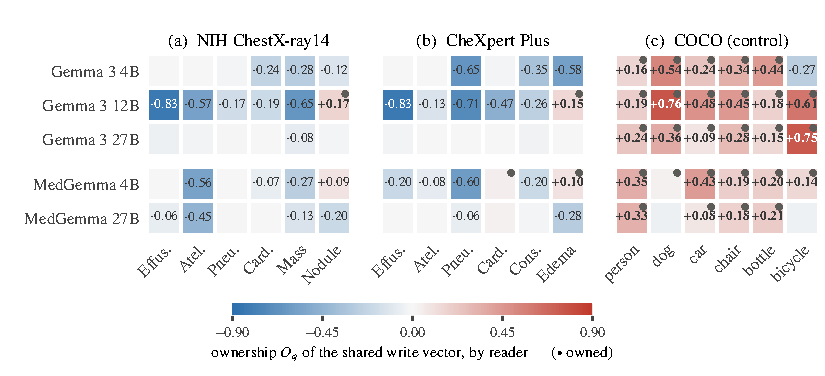
\includegraphics[width=\textwidth]{figures/fig5_same_write.pdf}
    \caption{\textbf{Same write, different reader.} Ownership $O_q$ per concept on NIH, CheXpert, and COCO for Gemma~3 4B/12B/27B and MedGemma 4B/27B, whose probes and write vectors are identical across sizes within each family; dots mark owned cells and hatching marks ceiling cells (clean answer beyond $0.99$ or $0.01$ on more than 90\% of rows).}
    \label{fig:readers}
\end{figure}

\subsection{The direction the reader responds to}
\label{sec:ansdir}

The same representation contains the reader's handle. For each question, we use ridge regression to fit the model's own clean answer margin from the same projected, train-scaled features, using the first 3{,}000 rows of the training cohort in fixed manifest order. This order is a seeded shuffle on NIH and a hash of patient or image identity on CheXpert and COCO; neither labels nor answers enter it. We select each question's penalty by five-fold cross-validated $R^2$ over $\{0.1,1,10,100\}$. Across the \cfAnsAlphaCells{} fitted questions, the selected penalty is $1$ for \cfAnsAlphaOne{}, $10$ for \cfAnsAlphaTen{}, and $100$ for \cfAnsAlphaHundred{}. Cross-validation splits rows. On CheXpert and COCO, each of the 3{,}000 rows represents a distinct patient or image. On NIH, the rows come from \cfAnsTrainUnitsNih{} patients. We lift the fitted direction as we lift a probe normal and write it at the same dose against the same reference family (Table~\ref{tab:cf-ansdir}). This answer direction $a_q$ is a handle where the label direction is not. Across the \cfAnsChestN{} chest cells in the \cfAnsChestBlocks{} scored chest blocks (Table~\ref{tab:cf-ansdir}, top), $a_q$ is owned in \cfAnsChestOwnedA{} and the label direction in \cfAnsChestOwnedLabel{}. The answer direction's write beats the strongest logistic competitor in \cfAnsChestBeats{}. Across the five held-out templates, $a_q$ remains owned in \cfAnsdirtChestKept{} of \cfAnsdirtChestKeptN{} chest and \cfAnsdirtCocoKept{} of \cfAnsdirtCocoKeptN{} COCO (cell, template) pairs (Table~\ref{tab:cf-ansdir}, bottom). Across all pairs, regardless of cell ownership under the primary template, $a_q$ is owned in \cfAnsdirtChestOwnedPairs{} of \cfAnsdirtChestPairsAll{} chest and \cfAnsdirtCocoOwnedPairs{} of \cfAnsdirtCocoPairsAll{} COCO (cell, template) pairs. In Qwen2.5-VL-7B, it is owned for \cfAnsQwenOwnedNih{} of six NIH concepts (Effusion $O^a=\cfAnsQwenEffO$ with an own write of $\cfAnsQwenEffW$) and all \cfAnsQwenOwnedChex{} CheXpert concepts. In Lingshu 32B, it is owned for \cfAnsLingOwnedNih{} NIH and \cfAnsLingOwnedChex{} CheXpert concepts. In Gemma~3 12B, it is owned for \cfAnsGemOwnedNih{} NIH and \cfAnsGemOwnedChex{} CheXpert concepts. We summarise the raw model-space cosine between the answer direction and the probe normal by the median over each block's six concepts. These medians span $\cfAnsCosQwenMin$--$\cfAnsCosQwenMax$ across the two chest blocks of Qwen2.5-VL-7B and $\cfAnsCosLingMin$--$\cfAnsCosLingMax$ across those of Lingshu 32B, compared with $\cfAnsCosCocoMin$--$\cfAnsCosCocoMax$ across the COCO blocks. The cosine whitened by the training-feature covariance in the projected, train-scaled space has a median over each dataset's cells of $\cfValCosSigmaChestMin$--$\cfValCosSigmaChestMax$ on the two chest sets and $\cfValCosSigmaCoco$ on COCO. The metrics differ most on the CheXpert block of Lingshu 32B, where the median over its six concepts is $\cfValCosRawLingChex$ raw and $\cfValCosSigmaLingChex$ whitened. The answer direction reads the model, not the label. Over the \cfValAurocAnsChestN{} chest cells, its median AUROC against the report label is $\cfValAurocAnsChest$, compared with $\cfValAurocProbeChest$ for the probe. Against the model's own clean answer, its median AUROC is $\cfValAurocAnsCleanChest$, compared with $\cfValAurocProbeCleanChest$ for the probe (median over the \cfValAurocAnsCleanChestN{} chest cells whose clean answers take both values; Table~\ref{tab:cf-validation}). In Qwen2.5-VL-7B on NIH, the label AUROC is $\cfValAurocAnsQwenNih$ for the answer direction and $\cfValAurocProbeQwenNih$ for the probe. The clean-answer AUROC is $\cfValAurocAnsCleanQwenNih$ and $\cfValAurocProbeCleanQwenNih$, respectively. Ownership compares the six directions of one construction within each question's row of $W$. The column-selectivity index $S_d=W_{d,d}/\sum_q|W_{q,d}|$ of Section~\ref{sec:robust-geometry} measures the share of a direction's effect that lands on its own question. Across the \cfAnsColSelChestN{} chest cells, the median $S_d$ is $\cfAnsColSelChest$ for answer directions and $\cfAnsColSelLabelChest$ for label directions in the same blocks. The corresponding medians are $\cfAnsColSelCoco$ and $\cfAnsColSelLabelCoco$ over the \cfAnsColSelCocoN{} COCO cells. On the chest sets, both answer and label directions move the other five answers along with their own. The row comparison separates them: the answer direction wins in \cfAnsChestOwnedA{} of \cfAnsChestN{} cells against \cfAnsChestOwnedLabel{} for the label direction. On natural images, the readable and writable directions coincide. On chest radiographs, the model answers along a direction the probe does not read.

We test writes from both families at four endpoints used to fit neither direction: the negated form of the concept's yes/no question, a two-alternative forced choice against the concept's strongest competitor in each of the two presentation orders, and the finding word's log-probability in a report continuation (Table~\ref{tab:cf-semend}). Across the \cfSemCells{} endpoint cells of the \cfSemBlocks{} scored blocks, the label direction is owned in \cfSemLabelOwned{} and the answer direction in \cfSemAnswerOwned{}. The negated question moves opposite to the affirmative one in \cfSemNegOpposite{} of the \cfSemNegN{} concept--block pairs. The forced choice is owned in both presentation orders in \cfSemForcedOwned{} of \cfSemForcedN{} pairs, with a mean absolute gap of \cfSemGapMin{}--\cfSemGapMax{} between orders. The report continuation is owned in \cfSemReportOwned{} of \cfSemReportCells{} cells. The separation between the two families persists across endpoints.

Ownership predicts endpoint effects beyond write magnitude, probe selectivity, and clean-answer AUROC. Regressing each endpoint effect on these three quantities with endpoint dummies gives a base $R^2$ of \cfSemIVBaseMin{}--\cfSemIVBaseMax{}. Adding the ownership contrast raises it by \cfSemIVMin{}--\cfSemIVMax{}. The added-variance interval excludes zero in all \cfSemIVExcl{} of the \cfSemIVN{} block-and-family combinations. Ownership is a predictive criterion, not a label.

\subsection{Size and family}
\label{sec:families}

Ownership on the chest sets is concentrated among a few readers and varies by concept and dataset (Figure~\ref{fig:ladders}; Table~\ref{tab:cf-models}). Qwen2.5-VL owns no concepts at 3B or 7B. At 32B, it owns Cardiomegaly. At 72B, it owns Atelectasis ($O=\cfOQwenSeventyTwoAtel$), Cardiomegaly, and Mass. Effusion is anti-owned at every size. Lingshu, the medical Qwen2.5-VL derivative, owns three CheXpert concepts at 7B. At 32B, it owns five, the highest clinical ownership in the grid. InternVL3.5 answers every NIH question at every size. On the chest sets, its writes remain within $\cfInternvlWqqMax$ of zero. LLaVA-1.5 reads the chest concepts. It answers none above chance. It owns none.

\subsection{Controls and alternatives}
\label{sec:controls}

The reference family and additional controls behave as designed across the grid (Figure~\ref{fig:overview}d; Table~\ref{tab:cf-controls}). Owned concept writes rank 1--6 among the 120 compared effects. The concept write typically ranks in the top decile on the chest sets.

\label{sec:robust-geometry}

\paragraph{Geometry, scale, saturation, refits, numerics.} No measurement alternative explains the deficit (Tables~\ref{tab:cf-geometry}--\ref{tab:cf-validation}; Appendix~\ref{app:cf-robustness}). The strongest competitor matches the most similar direction or the most co-occurring label at chance rate. Logit-scale verdicts agree in \cfScaleAgree{} of \cfScaleAgreeN{} cells. COCO blocks are more saturated than chest blocks. Restricting each cell to unsaturated rows preserves the full owned grade in \cfScaleUnsatGradeKept{} of \cfScaleUnsatGradeN{} owned chest cells. We recompute the steering reference on those rows. We evaluate the simultaneous max-$T$ advantage over the same six-direction family. Refits change $O_q$ by a median of \cfScaleRefitMedian{}. The column-selectivity index $S_d=W_{d,d}/\sum_q|W_{q,d}|$ divides a direction's signed effect on its own question by its summed absolute effect on the six questions. Across cells, its median is \cfValColSelNih{} on NIH and \cfValColSelChex{} on CheXpert, versus \cfValColSelCoco{} on COCO (Table~\ref{tab:cf-validation}). $S_d$ retains negative effects and weights every cell equally. It therefore differs from the write-flow share of Section~\ref{sec:deficit}, which retains only positive effects and pools them over checkpoints. On CheXpert, restricting evaluation to rows with a known label preserves the sign of $O_q$ in \cfValKnownSignAgree{} of \cfValKnownN{} cells. Re-grading the same fitted directions on \cfValidRows{} CheXpert films labelled by radiologist consensus reproduces the owned grade in \cfValidOwnedAgree{} of \cfValidCells{} cells (Table~\ref{tab:cf-valid}). These films share no patient with any campaign cohort. Both grades use directions fitted on report-derived labels. Refitting the six directions on the radiologist labels themselves changes the fit's label source. Across the \cfValidfitBlocks{} CheXpert blocks with this refit, the expert-label and report-label directions have a median raw model-space cosine of \cfValidfitCosRaw{} and a median whitened cosine of \cfValidfitCosWhitened{}. The expert-label refit reads the radiologist labels with a median cross-fitted AUROC of \cfValidfitAurocExpert{}, versus \cfValidfitAurocReportDir{} for the report-label direction on the same films. Written on the test rows under the same references, the expert-label directions are owned in \cfValidfitOwnedExpert{} of \cfValidfitCells{} cells, the report-label directions in \cfValidfitOwnedReport{} (Appendix~\ref{app:cf-robustness}). Rescoring in fp32 and at batch size one changes $W$ by at most \cfPrecisionMaxDW{} and alters \cfPrecisionGradeChanges{} of \cfPrecisionGradeCells{} grades (Table~\ref{tab:cf-precision}).

\paragraph{Alternative direction constructions.} The deficit persists beyond the logistic normal. We test four alternative directions with the same projected, train-scaled features and write protocol (Table~\ref{tab:cf-altdir}): the difference of class means, the Haufe pattern $\Sigma\boldsymbol\beta_c$ \citep{haufe2014interpretation}, the normal orthogonalised against the other five normals, and the normal refitted on features residualised against the other five labels. Across the \cfAltdirBlocks{} scored blocks (\cfAltdirBlocksPerDs{} per dataset), each construction owns \cfAltdirChestPctMin{}--\cfAltdirChestPctMax\% of chest cells and \cfAltdirCocoPctMin{}--\cfAltdirCocoPctMax\% of COCO cells. For the difference-of-means and pattern directions, we measure the absolute raw model-space cosine with the logistic normal. The median over the six concepts in each block ranges from $\cfAltdirCosMin$ to $\cfAltdirCosMax$. Each of these two directions owns more NIH cells and fewer COCO cells than the logistic normal. Lifted as displacements, they respectively own \cfAltdirdChestDom{} and \cfAltdirdChestPattern{} of \cfAltdirdChestN{} chest cells and \cfAltdirdCocoDom{} and \cfAltdirdCocoPattern{} of \cfAltdirdCocoN{} COCO cells (Table~\ref{tab:cf-altdir}). Every construction preserves the chest-to-COCO gap. At least one construction owns \cfAltdirNihAny{} of \cfAltdirNihN{} cells on NIH and \cfAltdirChexAny{} of \cfAltdirChexN{} on CheXpert, compared with \cfAltdirCocoAny{} of \cfAltdirCocoN{} on COCO. Extending the clinical family to every additional dataset label with enough support retains \cfExtcompRetained{} of the \cfExtcompOwned{} owned cells in the \cfExtcompBlocks{} scored blocks (Table~\ref{tab:cf-altdir}). We combine projection, sex, age, and the findings into one nine-direction family. The three attributes are non-clinical properties of the same radiographs. Their probes read them at least as well as the clinical probes read the findings. Median probe AUROC per attribute is \cfAttrAurocMin{}--\cfAttrAurocMax{}, compared with \cfAttrClinAuroc{} for findings in the same blocks. All \cfAttrReadable{} of \cfAttrChestAttrN{} attribute cells are readable. Both kinds of question carry the same steering reference in all \cfAttrRefBlocks{} blocks. Attributes own \cfAttrAllAttrOwned{} of \cfAttrAllAttrN{} cells; findings own \cfAttrAllClinOwned{} of \cfAttrAllClinN{}, the same rate. Among cells whose clean answer meets the answer-capable rule, attributes own \cfAttrCapAttrOwned{} of \cfAttrCapAttrN{} and findings \cfAttrCapClinOwned{} of \cfAttrCapClinN{}. Pairing each attribute cell with clinical cells from its own block within \cfAttrPairWindow{} clean-answer AUROC yields \cfAttrPairAttrN{} pairs, with attributes owned in \cfAttrPairAttrOwned{} and findings in \cfAttrPairClinOwned{}. The within-image comparison shows that a non-clinical property of the same film is no more writable than a finding. Each attribute question uses one of \cfAttrqPhrasings{} phrasings scored on the calibration rows. The written phrasing reaches a median clean-answer AUROC of \cfAttrqWrittenAuroc{} against \cfAttrqSelectedAuroc{} for the most answerable phrasing of the same cell. The median gap is \cfAttrqGain{} over the \cfAttrqCells{} attribute cells. On NIH, ownership is \cfAttrNihAttrOwned{}/\cfAttrNihAttrN{} for attributes and \cfAttrNihClinOwned{}/\cfAttrNihClinN{} for findings (Table~\ref{tab:cf-attr}). We weight writes along the logistic directions by the softmax of token probe scores or restrict them to the top quarter of tokens at four times the weight (twice the Frobenius norm of the uniform write). Across the \cfTokenwChestBlocks{} chest blocks with these writes, the softmax write owns \cfTokenwSoftChestOwned{} of \cfTokenwChestCells{} cells, the top-quarter write owns \cfTokenwTopqChestOwned{}, and the uniform write owns \cfTokenwUniformChestOwned{}. On COCO, the softmax and top-quarter writes own \cfTokenwSoftCocoOwned{} and \cfTokenwTopqCocoOwned{} of \cfTokenwCocoCells{} cells (Table~\ref{tab:cf-altdir}). Concentrating the write where the probe reads does not create a clinical handle.


\FloatBarrier

\section{Implications}
\label{sec:implications}

\paragraph{For steering, model building, and clinical evaluation.}
A probe direction that reads a clinical concept is not a handle on it, and probe accuracy and answer accuracy, the two quantities most often reported for medical VLMs, do not establish whether a handle exists: both are high in this grid, yet ownership is \cfChestOwnedPct\%. A steering study that beats random and sham controls shows that the write reaches the answer, not that the label names the direction; at the same locus, dose, and patients, a direction fitted for another finding moves the same answer as much or more in two thirds of clinical cells. The matched-competitor test is cheap once the competitors' directions exist: report the write matrix $W$ whenever probe normals are used as interventions, compare ownership $O_q$ across layers, doses, and models, and pair every clinical write with a natural-image control. The same write vector produces different ownership in different language models, so a vision tower that exposes a finding linearly does not make its direction a handle; ownership rises with the reader in some families and not in others (Gemma~3, InternVL3.5).

\section{Conclusion}
\label{sec:conclusion}

Reading a clinical concept from a vision-language model's visual representation does not make its probe direction a handle on that concept. Across \cfCheckpoints{} checkpoints and two chest-radiograph datasets, concepts are readable in \cfChestReadablePct\% and answerable in \cfChestAnswerablePct\% of cells but owned in \cfChestOwnedPct\%. The same procedure owns \cfCocoOwnedPct\% of natural-object cells. Non-clinical attributes of the same films are owned in \cfAttrAllAttrOwned{} of \cfAttrAllAttrN{} cells against \cfAttrAllClinOwned{} of \cfAttrAllClinN{} for findings, and in none of the \cfStratAttrTopN{} attribute cells the model answers well: the deficit follows the chest-radiograph representation and its reader, not the concept's clinical status. The model's answer direction is a handle. On chest radiographs, it is nearly orthogonal to the probe direction in raw model space (cosine $\cfAnsCosChestMed$) and far from it under the training-feature covariance (whitened cosine $\cfValCosSigmaChestMin$--$\cfValCosSigmaChestMax$), compared with $\cfAnsCosCocoMed$ and $\cfValCosSigmaCoco$ on natural images. Checkpoints sharing a vision tower differ in what they own. Crossing the tower with the reader leaves every clinical concept unwritable in all four combinations. Ownership therefore rests on how the reader uses the representation.
\section*{Reproducibility statement}
The registered protocol file fixes the loci, projection, probe settings, dose grid, reference family, templates, modules, gates, and decision rules; its identifier and code commit are recorded in every block's scorecard. The release contains the evaluation code and adapters, the protocol file, the cohort manifests with their seeds, the fitted directions, the per-image outcomes of every module, every block's scorecard and coverage file, the rendered prompts, and the pinned checkpoint revisions (Table~\ref{tab:cf-models}); every table and figure in the paper is regenerated from those files by the scripts in the release.

\section*{Ethics statement}
The study uses three public datasets under their published terms: NIH ChestX-ray14 (NIH Clinical Center), CheXpert Plus (Stanford AIMI, accessed through its data-use agreement), and COCO (annotations CC BY 4.0). All radiographs are de-identified by their providers; no protected health information was accessed, and no image or report is redistributed. The write test evaluates model behaviour under activation edits and is not a diagnostic tool; its grades describe what a probe direction does inside a model and carry no claim of clinical benefit.

\bibliography{refs}
\bibliographystyle{plainnat}

\clearpage
\appendix
\section{Campaign details}
\label{app:campaign}

This appendix lists the checkpoints and their consumed loci, the acceptance decisions, the coverage of the campaign, and the per-concept results of every completed block.

\subsection{Labels, registration, and artifact}
\label{app:cf-labels}

\paragraph{Labels.} We use the report-derived labels supplied with each dataset (NIH ChestX-ray14 finding labels; the CheXpert labeler output distributed with CheXpert Plus; COCO instance annotations). A row is positive for label 1, negative for label 0, and \emph{unknown} when the labeler output is uncertain or blank. We exclude unknown rows from probe fitting, selectivity, and answer AUROC. We write and score them like all other rows. Fixed manifests drawn with recorded seeds define the cohorts. Training and test cohorts are patient-disjoint. Every cohort is disjoint from every seed-study cohort. Table~\ref{tab:cf-prevalence} gives per-concept counts. A second CheXpert cohort contains \cfValidRows{} frontal films from the CheXpert validation set, one per patient, with the radiologists' consensus labels. It has zero patient overlap with any campaign cohort (Table~\ref{tab:cf-valid}).

\paragraph{Registration.} We froze the protocol before scoring any grid block. The loci, projection and probe settings, dose, reference family, six templates, module set, seven gates, and three decision rules match the registered protocol file and its code commit. We registered the seed study's crossover and confirmation analyses before running them (Appendix~\ref{app:seed}). One analysis pass over the packaged outcomes produces everything reported per block. After completing the grid, we added the leaderboard, write-flow share, and per-image examples as descriptive summaries of these outputs.

\paragraph{Artifact.} The release includes evaluation code and adapters, the registered protocol file, cohort manifests with their seeds, fitted directions, per-image outcomes for every module (write, dose, refit, locus, and template rows), scorecards and coverage files for every block, and rendered prompts. Adding a new checkpoint requires one adapter that identifies the block it consumes and passes the gates.

\subsection{Grid and consumed loci}
\label{app:cf-grid}

\begin{table}[h]
\centering
\scriptsize
\setlength{\tabcolsep}{3pt}
\caption{\textbf{Checkpoint sheet.} Family, parameters, vision tower, consumed visual tokens per image at the primary locus, input image size, eligible question templates after the image-free mapping gate (I/W: ``is''/``show'' wording; Y: yes/no; A/B: letter mappings), completed dataset blocks, and GPU-hours of scoring (A100-80GB).}
\label{tab:cf-models}
\resizebox{\textwidth}{!}{%
\begin{tabular}{llrllllr}
\toprule
Checkpoint & Family & Params & Vision tower & Tokens & Image & Templates & Blocks (GPU-h) \\
\midrule
Qwen2.5-VL-3B & Qwen2.5-VL & 3B & native ViT 675M & 576$\to$144 & $336^2$ & IYWYIAWA & NIH (13), CXP (3), COCO (13) \\
Qwen2.5-VL-7B & Qwen2.5-VL & 7B & native ViT 675M & 576$\to$144 & $336^2$ & all & NIH (27), CXP (5), COCO (26) \\
Qwen2.5-VL-32B & Qwen2.5-VL & 32B & native ViT 675M & 576$\to$144 & $336^2$ & all & NIH (83), CXP (16), COCO (75) \\
Qwen2.5-VL-72B & Qwen2.5-VL & 72B & native ViT 675M & 576$\to$144 & $336^2$ & all & NIH (214) \\
Qwen3-VL-4B & Qwen3-VL & 4B & SigLIP2-based & $\leq$1024 & $\leq 512^2$ & all & NIH (15), CXP (3), COCO (14) \\
Qwen3-VL-8B & Qwen3-VL & 8B & SigLIP2-based & $\leq$1024 & $\leq 512^2$ & all & NIH (26), CXP (5), COCO (20) \\
Qwen3-VL-32B & Qwen3-VL & 32B & SigLIP2-based & $\leq$1024 & $\leq 512^2$ & all & NIH (106), CXP (28), COCO (98) \\
InternVL3.5-8B & InternVL3.5 & 8B & InternViT-300M & 1024 & $448^2$ & all & NIH (19), CXP (4), COCO (18) \\
InternVL3.5-14B & InternVL3.5 & 14B & InternViT-300M & 1024 & $448^2$ & all & NIH (29), CXP (5), COCO (28) \\
Gemma 3 4B & Gemma 3 & 4B & SigLIP-So400m & 4096 & $896^2$ & all & NIH (22), CXP (9), COCO (34) \\
Gemma 3 12B & Gemma 3 & 12B & SigLIP-So400m & 4096 & $896^2$ & all & NIH (40), CXP (11), COCO (52) \\
Gemma 3 27B & Gemma 3 & 27B & SigLIP-So400m & 4096 & $896^2$ & all & NIH (129), CXP (29), COCO (119) \\
MedGemma 4B & MedGemma & 4B & MedSigLIP & 4096 & $896^2$ & all & NIH (44), CXP (9), COCO (36) \\
MedGemma 27B & MedGemma & 27B & MedSigLIP & 4096 & $896^2$ & all & NIH (118), CXP (33), COCO (74) \\
Lingshu 7B & Lingshu & 7B & Qwen2.5-VL ViT & 576$\to$144 & $336^2$ & all & NIH (20), CXP (5), COCO (20) \\
Lingshu 32B & Lingshu & 32B & Qwen2.5-VL ViT & 576$\to$144 & $336^2$ & all & NIH (74), CXP (19), COCO (76) \\
LLaVA-1.5-7B & LLaVA-1.5 & 7B & CLIP ViT-L/14-336 & 576 & $336^2$ & IYWY & NIH (21), CXP (7), COCO (20) \\
LLaVA-1.5-13B & LLaVA-1.5 & 13B & CLIP ViT-L/14-336 & 576 & $336^2$ & IYWYIAWA & NIH (34), CXP (10), COCO (38) \\
LLaVA-Med 1.5 7B & LLaVA-Med & 7B & CLIP ViT-L/14-336 & 576 & $336^2$ & IYWY & NIH (20), CXP (7), COCO (22) \\
Llama 3.2 Vision 11B & Llama 3.2 Vision & 11B & ViT-H/14 & 1601 & $560^2$ & IBWB & NIH (22), CXP (0), COCO (22) \\
\bottomrule
\end{tabular}}
\end{table}

\begin{table}[h]
\centering
\scriptsize
\setlength{\tabcolsep}{4pt}
\caption{\textbf{Preflight gates.} Each block is scored only after the seven checks below run on 16 held-out rows at both loci; the right column gives the range observed over all completed blocks.}
\label{tab:cf-gates}
\begin{tabular}{clp{4.3cm}p{6.0cm}}
\toprule
Gate & Name & Criterion & Observed \\
\midrule
A & Determinism & identical answer logits on a repeated forward & max difference 0 \\
B & Identity at $\alpha=0$ & the armed hook with zero dose changes nothing & max difference 0 \\
C & Reach & the write changes the consumer input and the answer logits; no change outside consumed tokens & consumer change 0.44--29.84; answer logits 0.20--23.82; outside consumed tokens 0 \\
D & Batch consistency & single- vs batched-forward answer logits within 0.25 & 0.07--1.84; above tolerance (declared, neutralised by fixed batch composition): Qwen2.5-VL ($\leq$0.37), Qwen3-VL ($\leq$1.41), InternVL3.5 ($\leq$0.62), Gemma 3 ($\leq$1.84), MedGemma ($\leq$0.56), Lingshu ($\leq$0.30), LLaVA-1.5 ($\leq$0.31), Llama 3.2 Vision ($\leq$0.41) \\
E & Semantic mapping & image-free ``present/absent'' statements map to the right answer token under each template & failing templates: LLaVA-1.5-13B: IBWB; LLaVA-1.5-7B: IAIBWAWB; LLaVA-Med 1.5 7B: IAIBWAWB; Llama 3.2 Vision 11B: IYWYIAWA; Qwen2.5-VL-3B: IBWB \\
F & Throughput & rows per second recorded for scheduling & 3.8--35 rows/s \\
G & fp32 answer logits & fp32 logits recomputed from the final hidden state agree with the model's bf16 logits & max difference 0.12 \\
\bottomrule
\end{tabular}
\end{table}

\begin{table}[t]
\centering
\scriptsize
\setlength{\tabcolsep}{3pt}
% Morandi tints for the cf-transfer tables (muted, low saturation); darker = larger value
\definecolor{cfSage1}{HTML}{EEF1EA}
\definecolor{cfSage2}{HTML}{D9E1D2}
\definecolor{cfSage3}{HTML}{C1CDB8}
\definecolor{cfSage4}{HTML}{A6B79C}
\definecolor{cfSlate1}{HTML}{ECEFF2}
\definecolor{cfSlate2}{HTML}{D3DAE2}
\definecolor{cfSlate3}{HTML}{B7C3D0}
\definecolor{cfSlate4}{HTML}{98A8B9}
\definecolor{cfTerra1}{HTML}{F5ECE9}
\definecolor{cfTerra2}{HTML}{E9D3CC}
\definecolor{cfTerra3}{HTML}{DAB5AA}
\definecolor{cfTerra4}{HTML}{C9968A}
\definecolor{cfOat1}{HTML}{F4EFE6}
\definecolor{cfOat2}{HTML}{E8DDC8}
\definecolor{cfGrey}{HTML}{E4E1DC}

\caption{\textbf{Families.} Vision tower, sizes evaluated, medical fine-tuning, consumed visual tokens per image at the primary locus, mean probe selectivity and clean-answer AUROC over clinical cells, owned clinical and COCO cells, and the mean of three controls over blocks: signed dose range of $O_q$ (DOSE module), refit SD over three seeds, and $|$connector-locus median $O_q|$. Owned counts are shaded slate (darker = larger share).}
\label{tab:cf-families}
\resizebox{\textwidth}{!}{%
\begin{tabular}{llllrrrrrrrr}
\toprule
Family & Vision tower & Sizes & Med. & Tokens & $\bar S$ & $\overline{\mathrm{AUROC}}$ & Owned clin. & Owned COCO & Dose & Refit SD & $|O_\mathrm{conn}|$ \\
\midrule
Qwen2.5-VL & native ViT 675M & 3B/7B/32B/72B & no & 576$\to$144 & 0.122 & 0.625 & \cellcolor{cfSlate2}4/42 & \cellcolor{cfSlate4}18/18 & +0.46 & 0.076 & 0.014 \\
Qwen3-VL & SigLIP2-based & 4B/8B/32B & no & $\leq$1024 & 0.137 & 0.735 & \cellcolor{cfSlate2}4/36 & \cellcolor{cfSlate4}18/18 & +0.50 & 0.042 & 0.006 \\
InternVL3.5 & InternViT-300M / InternViT-6B & 8B/14B/38B & no & 1024 & 0.125 & 0.807 & \cellcolor{cfSlate2}5/36 & \cellcolor{cfSlate4}17/18 & +0.04 & 0.004 & 0.004 \\
Gemma 3 & SigLIP-So400m & 4B/12B/27B & no & 4096 & 0.124 & 0.564 & \cellcolor{cfSlate2}2/36 & \cellcolor{cfSlate4}17/18 & +0.57 & 0.102 & 0.023 \\
MedGemma & MedSigLIP & 4B/27B & yes & 4096 & 0.164 & 0.835 & \cellcolor{cfSlate2}2/24 & \cellcolor{cfSlate3}10/12 & +0.39 & 0.068 & 0.006 \\
Lingshu & Qwen2.5-VL ViT & 7B/32B & yes & 576$\to$144 & 0.142 & 0.820 & \cellcolor{cfSlate4}11/24 & \cellcolor{cfSlate4}12/12 & +0.38 & 0.047 & 0.008 \\
LLaVA-1.5 & CLIP ViT-L/14-336 & 7B/13B & no & 576 & 0.124 & 0.516 & \cellcolor{cfSlate1}0/24 & \cellcolor{cfSlate3}7/12 & +0.06 & 0.010 & 0.021 \\
LLaVA-Med & CLIP ViT-L/14-336 & 7B & yes & 576 & 0.136 & 0.560 & \cellcolor{cfSlate2}1/12 & \cellcolor{cfSlate2}1/6 & +0.03 & 0.008 & 0.012 \\
Llama 3.2 Vision & ViT-H/14 & 11B & no & 1601 & 0.119 & 0.688 & \cellcolor{cfSlate1}0/12 & \cellcolor{cfSlate2}1/6 & +0.08 & 0.035 & 0.039 \\
\bottomrule
\end{tabular}}
\end{table}

\begin{figure}[h]
    \centering
    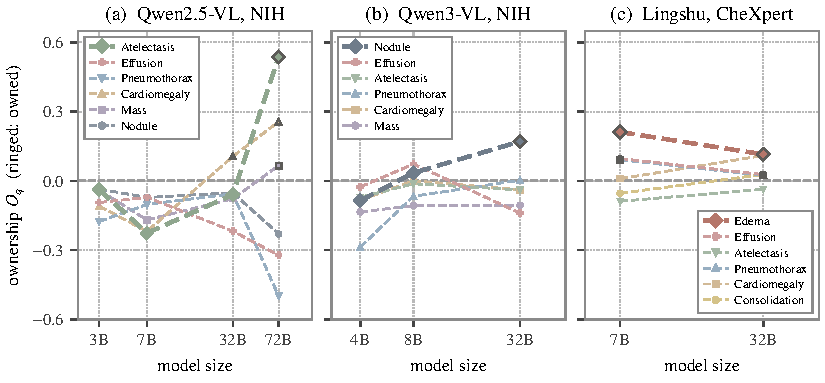
\includegraphics[width=\textwidth]{figures/fig6_ladders.pdf}
    \caption{\textbf{Size ladders.} Ownership $O_q$ per concept across sizes for Qwen2.5-VL on NIH, Qwen3-VL on NIH, and Lingshu on CheXpert. The concept with the largest ownership at the largest size is drawn bold (Atelectasis, Nodule, Edema); ringed markers are owned cells.}
    \label{fig:ladders}
\end{figure}

\begin{table}[h]
\centering
\scriptsize
\setlength{\tabcolsep}{4pt}
\caption{\textbf{Label counts per concept.} Positive / negative / unknown rows in the training and test cohorts of the fixed manifests (unknown = CheXpert labeler uncertain or blank; unknown rows are excluded from probe fitting, selectivity, and answer AUROC, and scored like every other row under every write).}
\label{tab:cf-prevalence}
\begin{tabular}{llrrrrrr}
\toprule
Dataset & Concept & \multicolumn{3}{c}{train (pos / neg / unk)} & \multicolumn{3}{c}{test (pos / neg / unk)} \\
\midrule
NIH ChestX-ray14 & Effusion & 2423 & 15789 & 0 & 46 & 554 & 0 \\
 & Atelectasis & 2311 & 15901 & 0 & 57 & 543 & 0 \\
 & Pneumothorax & 1254 & 16958 & 0 & 17 & 583 & 0 \\
 & Cardiomegaly & 881 & 17331 & 0 & 23 & 577 & 0 \\
 & Mass & 1263 & 16949 & 0 & 32 & 568 & 0 \\
 & Nodule & 1549 & 16663 & 0 & 47 & 553 & 0 \\
\addlinespace
CheXpert Plus & Effusion & 5897 & 4277 & 9826 & 158 & 130 & 312 \\
 & Atelectasis & 2891 & 86 & 17023 & 84 & 2 & 514 \\
 & Pneumothorax & 1086 & 6456 & 12458 & 32 & 213 & 355 \\
 & Cardiomegaly & 2312 & 1903 & 15785 & 71 & 58 & 471 \\
 & Consolidation & 966 & 3652 & 15382 & 25 & 113 & 462 \\
 & Edema & 3814 & 2231 & 13955 & 133 & 59 & 408 \\
\addlinespace
COCO & person & 10877 & 9123 & 0 & 321 & 279 & 0 \\
 & dog & 693 & 19307 & 0 & 15 & 585 & 0 \\
 & car & 2051 & 17949 & 0 & 60 & 540 & 0 \\
 & chair & 2183 & 17817 & 0 & 63 & 537 & 0 \\
 & bottle & 1455 & 18545 & 0 & 47 & 553 & 0 \\
 & bicycle & 567 & 19433 & 0 & 14 & 586 & 0 \\
\bottomrule
\end{tabular}
\end{table}


For Llama~3.2 Vision, the projector also reads five intermediate local-layer outputs that bypass the final global block. LLaVA computes the final CLIP block but consumes the penultimate block instead. For every checkpoint, Gate (C) verifies that the write reaches the consumer and the answer logits while changing nothing outside the consumed tokens.

\subsection{Acceptance decisions}
\label{app:cf-gates}

All \cfWriteBlocks{} completed blocks pass checks (A), (B), (C), and (G) with zero determinism error, zero change at $\alpha=0$, and fp32-versus-model logit differences below \cfGateFpMax{}. In check (D), the Qwen3-VL, Gemma~3, MedGemma, InternVL, and Llama families exceed the 0.25-logit tolerance (up to \cfGateBatchMax{} logits for Gemma~3 12B). We record these as declared deviations. Fixed batch composition neutralises them. Check (E) fails on all datasets for the A/B templates for LLaVA-1.5-7B and LLaVA-Med, the B-mapped templates for Qwen2.5-VL-3B and LLaVA-1.5-13B, and the yes/no and A-mapped templates for Llama~3.2 Vision 11B. We record the affected cells as ineligible. Two checkpoints answer ``yes'' to nearly every chest question (Gemma~3 4B: clean $P(\mathrm{yes})>0.99$ on \cfGemmaFourYesMin--\cfGemmaFourYesMax\% of rows). The answerability grade records this behaviour. Three checkpoints (LLaVA-1.5 7B/13B, LLaVA-Med) answer at chance.

\subsection{Coverage and cost}
\label{app:cf-coverage}

\cfCheckpointsCompleteWord{} checkpoints are complete on all three datasets (Table~\ref{tab:cf-coverage}). Coverage includes all modules on NIH and COCO---the write matrix, calibration, the five additional templates, the dose sweep, the two refits, and the connector locus---and the write matrix and calibration on CheXpert. We grade Llama~3.2 Vision 11B on its eligible B-positive template IB. Qwen2.5-VL-72B is complete on NIH. The compute budget prevented runs of the 72B COCO/CheXpert blocks and Llama~3.2 Vision 90B. InternVL3.5-38B is complete on all three datasets. The campaign used about 3,000 A100-hours. A chest block for a 7B checkpoint takes about ten GPU-hours.

\begin{table}[h]
\centering
\scriptsize
\setlength{\tabcolsep}{4pt}
\caption{\textbf{Coverage.} Modules completed per block at packaging (from the campaign manifest), with the modules whose template is ineligible (inel.) and the primary template when it is not the \emph{is}/yes-no template; ``--'' = block not run; modules still in progress are not listed. \cfCoverageBlocksAllSeven{} blocks carry all seven modules of the planned campaign, and the five modules added to CheXpert after the first wave are complete on \cfCoverageChexFull{} of the CheXpert blocks.}
\label{tab:cf-coverage}
\begin{tabular}{llll}
\toprule
Checkpoint & NIH ChestX-ray14 & CheXpert Plus & COCO \\
\midrule
Qwen2.5-VL-3B & C Cal P D R L Lc A Ad & C Cal A Ad & C Cal P D R L Lc A Ad \\
Qwen2.5-VL-7B & C Cal P D R L Lc A Ad An E T Pr & C Cal P D R L Lc A Ad An E T & C Cal P D R L Lc A Ad An T Pr \\
Qwen2.5-VL-32B & C Cal P D R L Lc A Ad & C Cal P D R L Lc A Ad & C Cal P D R L Lc A Ad \\
Qwen2.5-VL-72B & C Cal P D R L Lc & -- & -- \\
Qwen3-VL-4B & C Cal P D R L Lc A Ad & C Cal A Ad & C Cal P D R L Lc A Ad \\
Qwen3-VL-8B & C Cal P D R L Lc A Ad E T & C Cal A Ad & C Cal P D R L Lc A Ad T \\
Qwen3-VL-32B & C Cal P D R L Lc A Ad & C Cal D R Lc A Ad & C Cal P D R L Lc A Ad \\
InternVL3.5-8B & C Cal P D R L Lc A Ad E & C Cal A Ad & C Cal P D R L Lc A Ad \\
InternVL3.5-14B & C Cal P D R L Lc A Ad & C Cal A Ad & C Cal P D R L Lc A Ad \\
InternVL3.5-38B & C Cal P D R L Lc A & C Cal A & C Cal P D R L Lc A \\
Gemma 3 4B & C Cal P D R L Lc A Ad & C Cal A Ad & C Cal P D R L Lc A Ad \\
Gemma 3 12B & C Cal P D R L Lc A Ad An E T & C Cal A Ad An E & C Cal P D R L Lc A Ad An \\
Gemma 3 27B & C Cal P D R L Lc & C Cal A & C Cal P D R L Lc A \\
MedGemma 4B & C Cal P D R L Lc A Ad & C Cal A Ad E & C Cal P D R L Lc A Ad \\
MedGemma 27B & C Cal P D R L Lc A Ad & C Cal A & C Cal P D R L Lc A \\
Lingshu 7B & C Cal P D R L Lc A Ad & C Cal D R Lc A Ad & C Cal P D R L Lc A Ad \\
Lingshu 32B & C Cal P D R L Lc A Ad An E & C Cal A Ad An E & C Cal P D R L Lc A Ad An \\
LLaVA-1.5-7B & C Cal P D R L Lc A Ad & C Cal P D R L Lc A Ad & C Cal P D R L Lc A Ad \\
LLaVA-1.5-13B & C Cal P D R L Lc A Ad & C Cal A Ad & C Cal P D R L Lc A Ad \\
LLaVA-Med 1.5 7B & C Cal P D R L Lc A Ad & C Cal A Ad & C Cal P D R L Lc A Ad \\
Llama 3.2 Vision 11B & C Cal P D R L Lc A [IB] & C Cal D R L Lc A [IB] & C Cal P D R L Lc A [IB] \\
\midrule
\multicolumn{4}{p{0.95\textwidth}}{\textit{Legend:} C = CORE, Cal = CALIBRATION, P = PROMPT, D = DOSE, R = REFIT, L = LOCUS, Lc = LOCUS\_CALIBRATION, A = ALTDIR, Ad = ALTDIRD, An = ANSDIR, E = EXTCOMP, T = TOKENW, Pr = PRECISION.} \\
\bottomrule
\end{tabular}
\end{table}


\subsection{Ownership of every concept}
\label{app:cf-tables}

Tables~\ref{tab:cf-own-nih}--\ref{tab:cf-own-coco} report the ownership contrast for every concept cell. Figure~\ref{fig:cf-w-structure} summarises the structure of the underlying write matrices. Figure~\ref{fig:cf-examples} shows grades for individual images.

\begin{table}[h]
\centering
\scriptsize
\setlength{\tabcolsep}{4pt}
\renewcommand{\arraystretch}{1.08}
% Morandi tints for the cf-transfer tables (muted, low saturation); darker = larger value
\definecolor{cfSage1}{HTML}{EEF1EA}
\definecolor{cfSage2}{HTML}{D9E1D2}
\definecolor{cfSage3}{HTML}{C1CDB8}
\definecolor{cfSage4}{HTML}{A6B79C}
\definecolor{cfSlate1}{HTML}{ECEFF2}
\definecolor{cfSlate2}{HTML}{D3DAE2}
\definecolor{cfSlate3}{HTML}{B7C3D0}
\definecolor{cfSlate4}{HTML}{98A8B9}
\definecolor{cfTerra1}{HTML}{F5ECE9}
\definecolor{cfTerra2}{HTML}{E9D3CC}
\definecolor{cfTerra3}{HTML}{DAB5AA}
\definecolor{cfTerra4}{HTML}{C9968A}
\definecolor{cfOat1}{HTML}{F4EFE6}
\definecolor{cfOat2}{HTML}{E8DDC8}
\definecolor{cfGrey}{HTML}{E4E1DC}

\caption{\textbf{Ownership on NIH ChestX-ray14.} Each cell is the ownership contrast $O_q$ of the concept's own write against its strongest clinical competitor at $\alpha=+0.25$. Cells are shaded slate for positive and terracotta for negative values (darker = larger magnitude, thresholds $0.02$, $0.10$, $0.25$). Bold marks owned cells (steering reference met and all simultaneous lower bounds $>0$). A dagger marks cells whose write meets the steering reference but loses to a competitor. Grey ``inel.'' marks checkpoints whose yes/no template is ineligible. Checkpoints are in the order of Table~\ref{tab:cf-main}.}
\label{tab:cf-own-nih}
\begin{tabular}{lrrrrrr}
\toprule
Checkpoint & Effusion & Atelectasis & Pneumothorax & Cardiomegaly & Mass & Nodule \\
\midrule
Lingshu 32B & \cellcolor{cfTerra1}-0.01 & \cellcolor{cfTerra2}-0.08 & \cellcolor{cfSlate3}\textbf{+0.14} & \cellcolor{cfSlate2}\textbf{+0.05} & \cellcolor{cfTerra2}-0.08 & \cellcolor{cfTerra3}-0.18 \\
Qwen2.5-VL-72B & \cellcolor{cfTerra4}-0.32 & \cellcolor{cfSlate4}\textbf{+0.54} & \cellcolor{cfTerra4}-0.50 & \cellcolor{cfSlate4}\textbf{+0.26} & \cellcolor{cfSlate2}\textbf{+0.07} & \cellcolor{cfTerra3}-0.23 \\
Lingshu 7B & \cellcolor{cfSlate1}+0.02 & \cellcolor{cfSlate1}+0.01 & \cellcolor{cfSlate1}+0.01 & \cellcolor{cfSlate3}\textbf{+0.17} & \cellcolor{cfTerra2}-0.09 & \cellcolor{cfSlate1}+0.02 \\
Qwen3-VL-4B & \cellcolor{cfTerra2}-0.03$^{\dagger}$ & \cellcolor{cfTerra2}-0.07 & \cellcolor{cfTerra4}-0.29 & \cellcolor{cfTerra2}-0.08 & \cellcolor{cfTerra3}-0.13 & \cellcolor{cfTerra2}-0.09 \\
Qwen3-VL-32B & \cellcolor{cfTerra3}-0.14 & \cellcolor{cfTerra2}-0.04 & \cellcolor{cfSlate1}+0.00$^{\dagger}$ & \cellcolor{cfTerra2}-0.04 & \cellcolor{cfTerra3}-0.11 & \cellcolor{cfSlate3}\textbf{+0.17} \\
Gemma 3 12B & \cellcolor{cfTerra4}-0.83 & \cellcolor{cfTerra4}-0.57 & \cellcolor{cfTerra3}-0.17 & \cellcolor{cfTerra3}-0.19 & \cellcolor{cfTerra4}-0.65 & \cellcolor{cfSlate3}\textbf{+0.17} \\
MedGemma 4B & \cellcolor{cfSlate1}+0.01 & \cellcolor{cfTerra4}-0.56 & \cellcolor{cfSlate1}+0.01 & \cellcolor{cfTerra2}-0.07 & \cellcolor{cfTerra4}-0.27 & \cellcolor{cfSlate2}+0.09 \\
InternVL3.5-14B & \cellcolor{cfSlate1}\textbf{+0.01} & \cellcolor{cfTerra1}-0.01 & \cellcolor{cfTerra1}-0.00 & \cellcolor{cfTerra1}-0.00 & \cellcolor{cfSlate1}+0.00 & \cellcolor{cfTerra1}-0.01 \\
Qwen2.5-VL-32B & \cellcolor{cfTerra3}-0.22 & \cellcolor{cfTerra2}-0.06 & \cellcolor{cfTerra2}-0.06 & \cellcolor{cfSlate3}\textbf{+0.11} & \cellcolor{cfTerra2}-0.08 & \cellcolor{cfTerra2}-0.05 \\
InternVL3.5-8B & \cellcolor{cfSlate1}+0.00 & \cellcolor{cfTerra1}-0.02 & \cellcolor{cfTerra1}-0.00 & \cellcolor{cfSlate1}+0.00 & \cellcolor{cfTerra1}-0.01 & \cellcolor{cfTerra1}-0.01 \\
LLaVA-Med 1.5 7B & \cellcolor{cfTerra1}-0.00 & \cellcolor{cfTerra1}-0.00 & \cellcolor{cfTerra2}-0.04 & \cellcolor{cfTerra1}-0.01 & \cellcolor{cfTerra1}-0.01 & \cellcolor{cfTerra2}-0.02 \\
Qwen2.5-VL-3B & \cellcolor{cfTerra2}-0.09 & \cellcolor{cfTerra2}-0.04 & \cellcolor{cfTerra3}-0.18 & \cellcolor{cfTerra3}-0.11 & \cellcolor{cfTerra2}-0.04 & \cellcolor{cfTerra2}-0.04 \\
Qwen2.5-VL-7B & \cellcolor{cfTerra2}-0.07$^{\dagger}$ & \cellcolor{cfTerra3}-0.23 & \cellcolor{cfTerra3}-0.10 & \cellcolor{cfTerra3}-0.22 & \cellcolor{cfTerra3}-0.17 & \cellcolor{cfTerra2}-0.07 \\
Qwen3-VL-8B & \cellcolor{cfSlate2}+0.07 & \cellcolor{cfTerra1}-0.01 & \cellcolor{cfTerra2}-0.07 & \cellcolor{cfSlate1}+0.00 & \cellcolor{cfTerra3}-0.11 & \cellcolor{cfSlate2}+0.03 \\
InternVL3.5-38B & \cellcolor{cfSlate1}+0.00$^{\dagger}$ & \cellcolor{cfTerra1}-0.02 & \cellcolor{cfTerra1}-0.00 & \cellcolor{cfTerra2}-0.03 & \cellcolor{cfSlate1}+0.02 & \cellcolor{cfSlate1}+0.00 \\
Gemma 3 27B & \cellcolor{cfTerra2}-0.04 & \cellcolor{cfTerra2}-0.03 & \cellcolor{cfTerra1}-0.01 & \cellcolor{cfSlate1}+0.00$^{\dagger}$ & \cellcolor{cfTerra2}-0.08 & \cellcolor{cfTerra1}-0.02 \\
Gemma 3 4B & \cellcolor{cfTerra1}-0.00 & \cellcolor{cfTerra1}-0.00 & \cellcolor{cfTerra1}-0.01 & \cellcolor{cfTerra3}-0.24 & \cellcolor{cfTerra4}-0.28 & \cellcolor{cfTerra3}-0.12 \\
LLaVA-1.5-7B & \cellcolor{cfTerra2}-0.03 & \cellcolor{cfTerra1}-0.01 & \cellcolor{cfTerra2}-0.08 & \cellcolor{cfTerra3}-0.13 & \cellcolor{cfSlate2}+0.02 & \cellcolor{cfTerra1}-0.02 \\
MedGemma 27B & \cellcolor{cfTerra2}-0.06 & \cellcolor{cfTerra4}-0.45 & \cellcolor{cfTerra1}-0.01 & \cellcolor{cfSlate1}+0.00 & \cellcolor{cfTerra3}-0.13 & \cellcolor{cfTerra3}-0.20 \\
LLaVA-1.5-13B & \cellcolor{cfTerra1}-0.01 & \cellcolor{cfTerra2}-0.05 & \cellcolor{cfTerra2}-0.04 & \cellcolor{cfTerra2}-0.03 & \cellcolor{cfSlate1}+0.01 & \cellcolor{cfTerra1}-0.02 \\
Llama 3.2 Vision 11B & \cellcolor{cfTerra2}-0.04 & \cellcolor{cfTerra2}-0.07 & \cellcolor{cfTerra2}-0.05 & \cellcolor{cfSlate2}+0.02 & \cellcolor{cfTerra2}-0.06 & \cellcolor{cfTerra1}-0.01 \\
\midrule
\textbf{Owned} & 1 & 1 & 1 & 4 & 1 & 2 \\
\bottomrule
\end{tabular}
\end{table}

\begin{table}[h]
\centering
\scriptsize
\setlength{\tabcolsep}{4pt}
\renewcommand{\arraystretch}{1.08}
% Morandi tints for the cf-transfer tables (muted, low saturation); darker = larger value
\definecolor{cfSage1}{HTML}{EEF1EA}
\definecolor{cfSage2}{HTML}{D9E1D2}
\definecolor{cfSage3}{HTML}{C1CDB8}
\definecolor{cfSage4}{HTML}{A6B79C}
\definecolor{cfSlate1}{HTML}{ECEFF2}
\definecolor{cfSlate2}{HTML}{D3DAE2}
\definecolor{cfSlate3}{HTML}{B7C3D0}
\definecolor{cfSlate4}{HTML}{98A8B9}
\definecolor{cfTerra1}{HTML}{F5ECE9}
\definecolor{cfTerra2}{HTML}{E9D3CC}
\definecolor{cfTerra3}{HTML}{DAB5AA}
\definecolor{cfTerra4}{HTML}{C9968A}
\definecolor{cfOat1}{HTML}{F4EFE6}
\definecolor{cfOat2}{HTML}{E8DDC8}
\definecolor{cfGrey}{HTML}{E4E1DC}

\caption{\textbf{Ownership on CheXpert Plus.} Each cell is the ownership contrast $O_q$ of the concept's own write against its strongest clinical competitor at $\alpha=+0.25$. Cells are shaded slate for positive and terracotta for negative values (darker = larger magnitude, thresholds $0.02$, $0.10$, $0.25$). Bold marks owned cells (steering reference met and all simultaneous lower bounds $>0$). A dagger marks cells whose write meets the steering reference but has a stronger competitor; a double dagger marks reference-meeting cells whose comparison is unresolved. Grey ``inel.'' marks checkpoints whose yes/no template is ineligible and grey ``inc.'' a write matrix incomplete at packaging (neither enters any count). Checkpoints are in the order of Table~\ref{tab:cf-main}.}
\label{tab:cf-own-chexpert}
\begin{tabular}{lrrrrrr}
\toprule
Checkpoint & Effusion & Atelectasis & Pneumothorax & Cardiomegaly & Consolidation & Edema \\
\midrule
Lingshu 32B & \cellcolor{cfSlate2}\textbf{+0.03} & \cellcolor{cfTerra2}-0.04$^{\dagger}$ & \cellcolor{cfSlate2}\textbf{+0.02} & \cellcolor{cfSlate3}\textbf{+0.11} & \cellcolor{cfSlate2}\textbf{+0.03} & \cellcolor{cfSlate3}\textbf{+0.11} \\
Lingshu 7B & \cellcolor{cfSlate2}\textbf{+0.10} & \cellcolor{cfTerra2}-0.09 & \cellcolor{cfSlate2}\textbf{+0.09} & \cellcolor{cfSlate1}+0.01$^{\ddagger}$ & \cellcolor{cfTerra2}-0.05 & \cellcolor{cfSlate3}\textbf{+0.21} \\
Qwen3-VL-4B & \cellcolor{cfTerra1}-0.01$^{\dagger}$ & \cellcolor{cfTerra1}-0.02 & \cellcolor{cfTerra3}-0.23 & \cellcolor{cfTerra1}-0.01 & \cellcolor{cfSlate2}\textbf{+0.09} & \cellcolor{cfSlate2}\textbf{+0.09} \\
Qwen3-VL-32B & \cellcolor{cfTerra2}-0.04 & \cellcolor{cfSlate1}+0.00$^{\ddagger}$ & \cellcolor{cfSlate1}+0.00 & \cellcolor{cfTerra2}-0.03 & \cellcolor{cfTerra3}-0.12 & \cellcolor{cfSlate2}\textbf{+0.05} \\
InternVL3.5-38B & \cellcolor{cfSlate1}\textbf{+0.02} & \cellcolor{cfTerra1}-0.01 & \cellcolor{cfTerra1}-0.00 & \cellcolor{cfTerra1}-0.00$^{\ddagger}$ & \cellcolor{cfSlate1}\textbf{+0.01} & \cellcolor{cfTerra2}-0.02 \\
Gemma 3 12B & \cellcolor{cfTerra4}-0.83 & \cellcolor{cfTerra3}-0.13 & \cellcolor{cfTerra4}-0.71 & \cellcolor{cfTerra4}-0.47 & \cellcolor{cfTerra4}-0.26 & \cellcolor{cfSlate3}\textbf{+0.15} \\
MedGemma 4B & \cellcolor{cfTerra3}-0.20 & \cellcolor{cfTerra2}-0.08 & \cellcolor{cfTerra4}-0.60 & \cellcolor{cfSlate2}\textbf{+0.04} & \cellcolor{cfTerra3}-0.20 & \cellcolor{cfSlate3}\textbf{+0.10} \\
InternVL3.5-14B & \cellcolor{cfSlate1}\textbf{+0.01} & \cellcolor{cfTerra1}-0.00 & \cellcolor{cfSlate1}+0.00 & \cellcolor{cfTerra1}-0.01 & \cellcolor{cfSlate1}+0.01 & \cellcolor{cfTerra1}-0.00 \\
Qwen2.5-VL-32B & \cellcolor{cfTerra2}-0.07 & \cellcolor{cfTerra3}-0.19 & \cellcolor{cfTerra3}-0.12 & \cellcolor{cfTerra3}-0.19 & \cellcolor{cfTerra2}-0.05 & \cellcolor{cfTerra2}-0.02 \\
InternVL3.5-8B & \cellcolor{cfTerra1}-0.01 & \cellcolor{cfTerra1}-0.01 & \cellcolor{cfSlate1}\textbf{+0.00} & \cellcolor{cfTerra1}-0.00 & \cellcolor{cfSlate1}+0.01 & \cellcolor{cfTerra1}-0.00 \\
LLaVA-Med 1.5 7B & \cellcolor{cfSlate1}\textbf{+0.00} & \cellcolor{cfTerra1}-0.00 & \cellcolor{cfTerra2}-0.02 & \cellcolor{cfTerra2}-0.03 & \cellcolor{cfTerra1}-0.00$^{\dagger}$ & \cellcolor{cfTerra1}-0.02 \\
Qwen2.5-VL-3B & \cellcolor{cfTerra3}-0.18 & \cellcolor{cfTerra1}-0.02 & \cellcolor{cfTerra2}-0.04 & \cellcolor{cfTerra2}-0.05 & \cellcolor{cfTerra2}-0.03 & \cellcolor{cfTerra2}-0.08 \\
Qwen2.5-VL-7B & \cellcolor{cfSlate1}+0.01 & \cellcolor{cfTerra2}-0.05 & \cellcolor{cfTerra2}-0.10 & \cellcolor{cfTerra1}-0.00 & \cellcolor{cfTerra3}-0.15 & \cellcolor{cfTerra3}-0.18 \\
Qwen3-VL-8B & \cellcolor{cfTerra2}-0.07$^{\dagger}$ & \cellcolor{cfTerra1}-0.00$^{\dagger}$ & \cellcolor{cfTerra2}-0.10 & \cellcolor{cfTerra1}-0.00 & \cellcolor{cfTerra2}-0.04$^{\dagger}$ & \cellcolor{cfTerra2}-0.06 \\
Gemma 3 27B & \cellcolor{cfTerra2}-0.03 & \cellcolor{cfTerra1}-0.00 & \cellcolor{cfTerra1}-0.01 & \cellcolor{cfTerra1}-0.00 & \cellcolor{cfTerra2}-0.03 & \cellcolor{cfSlate1}+0.00$^{\ddagger}$ \\
Gemma 3 4B & \cellcolor{cfTerra1}-0.00 & \cellcolor{cfTerra1}-0.00 & \cellcolor{cfTerra4}-0.65 & \cellcolor{cfTerra1}-0.02 & \cellcolor{cfTerra4}-0.35 & \cellcolor{cfTerra4}-0.58 \\
LLaVA-1.5-7B & \cellcolor{cfSlate1}+0.00 & \cellcolor{cfTerra2}-0.09 & \cellcolor{cfTerra2}-0.10 & \cellcolor{cfSlate2}+0.03 & \cellcolor{cfTerra2}-0.03 & \cellcolor{cfTerra1}-0.00 \\
MedGemma 27B & \cellcolor{cfTerra1}-0.01 & \cellcolor{cfSlate1}+0.00 & \cellcolor{cfTerra2}-0.06 & \cellcolor{cfSlate2}+0.03 & \cellcolor{cfTerra1}-0.02 & \cellcolor{cfTerra4}-0.28 \\
LLaVA-1.5-13B & \cellcolor{cfTerra1}-0.00 & \cellcolor{cfTerra2}-0.03 & \cellcolor{cfTerra1}-0.01 & \cellcolor{cfSlate1}+0.00 & \cellcolor{cfSlate1}+0.01 & \cellcolor{cfTerra1}-0.01 \\
Llama 3.2 Vision 11B & \cellcolor{cfGrey}inel. & \cellcolor{cfGrey}inel. & \cellcolor{cfGrey}inel. & \cellcolor{cfGrey}inel. & \cellcolor{cfGrey}inel. & \cellcolor{cfGrey}inel. \\
\midrule
\textbf{Owned} & 5 & 0 & 3 & 2 & 3 & 6 \\
\bottomrule
\end{tabular}
\end{table}

\begin{table}[h]
\centering
\scriptsize
\setlength{\tabcolsep}{4pt}
\renewcommand{\arraystretch}{1.08}
% Morandi tints for the cf-transfer tables (muted, low saturation); darker = larger value
\definecolor{cfSage1}{HTML}{EEF1EA}
\definecolor{cfSage2}{HTML}{D9E1D2}
\definecolor{cfSage3}{HTML}{C1CDB8}
\definecolor{cfSage4}{HTML}{A6B79C}
\definecolor{cfSlate1}{HTML}{ECEFF2}
\definecolor{cfSlate2}{HTML}{D3DAE2}
\definecolor{cfSlate3}{HTML}{B7C3D0}
\definecolor{cfSlate4}{HTML}{98A8B9}
\definecolor{cfTerra1}{HTML}{F5ECE9}
\definecolor{cfTerra2}{HTML}{E9D3CC}
\definecolor{cfTerra3}{HTML}{DAB5AA}
\definecolor{cfTerra4}{HTML}{C9968A}
\definecolor{cfOat1}{HTML}{F4EFE6}
\definecolor{cfOat2}{HTML}{E8DDC8}
\definecolor{cfGrey}{HTML}{E4E1DC}

\caption{\textbf{Ownership on COCO.} Each cell is the ownership contrast $O_q$ of the concept's own write against its strongest clinical competitor at $\alpha=+0.25$. Cells are shaded slate for positive and terracotta for negative values (darker = larger magnitude, thresholds $0.02$, $0.10$, $0.25$). Bold marks owned cells (steering reference met and all simultaneous lower bounds $>0$). A dagger marks cells whose write meets the steering reference but loses to a competitor. Grey ``inel.'' marks checkpoints whose yes/no template is ineligible. Checkpoints are in the order of Table~\ref{tab:cf-main}.}
\label{tab:cf-own-coco}
\begin{tabular}{lrrrrrr}
\toprule
Checkpoint & person & dog & car & chair & bottle & bicycle \\
\midrule
Lingshu 32B & \cellcolor{cfSlate4}\textbf{+0.29} & \cellcolor{cfSlate3}\textbf{+0.23} & \cellcolor{cfSlate2}\textbf{+0.08} & \cellcolor{cfSlate4}\textbf{+0.53} & \cellcolor{cfSlate4}\textbf{+0.34} & \cellcolor{cfSlate3}\textbf{+0.22} \\
Lingshu 7B & \cellcolor{cfSlate4}\textbf{+0.39} & \cellcolor{cfSlate4}\textbf{+0.74} & \cellcolor{cfSlate4}\textbf{+0.70} & \cellcolor{cfSlate4}\textbf{+0.76} & \cellcolor{cfSlate4}\textbf{+0.64} & \cellcolor{cfSlate4}\textbf{+0.85} \\
Qwen3-VL-4B & \cellcolor{cfSlate4}\textbf{+0.46} & \cellcolor{cfSlate3}\textbf{+0.13} & \cellcolor{cfSlate4}\textbf{+0.33} & \cellcolor{cfSlate4}\textbf{+0.71} & \cellcolor{cfSlate4}\textbf{+0.34} & \cellcolor{cfSlate2}\textbf{+0.07} \\
Qwen3-VL-32B & \cellcolor{cfSlate3}\textbf{+0.13} & \cellcolor{cfSlate3}\textbf{+0.12} & \cellcolor{cfSlate3}\textbf{+0.11} & \cellcolor{cfSlate3}\textbf{+0.23} & \cellcolor{cfSlate3}\textbf{+0.24} & \cellcolor{cfSlate2}\textbf{+0.07} \\
InternVL3.5-38B & \cellcolor{cfSlate1}\textbf{+0.01} & \cellcolor{cfSlate1}\textbf{+0.00} & \cellcolor{cfSlate1}\textbf{+0.01} & \cellcolor{cfSlate1}\textbf{+0.02} & \cellcolor{cfSlate1}\textbf{+0.01} & \cellcolor{cfSlate1}\textbf{+0.01} \\
Gemma 3 12B & \cellcolor{cfSlate3}\textbf{+0.19} & \cellcolor{cfSlate4}\textbf{+0.76} & \cellcolor{cfSlate4}\textbf{+0.48} & \cellcolor{cfSlate4}\textbf{+0.45} & \cellcolor{cfSlate3}\textbf{+0.18} & \cellcolor{cfSlate4}\textbf{+0.61} \\
MedGemma 4B & \cellcolor{cfSlate4}\textbf{+0.35} & \cellcolor{cfSlate2}\textbf{+0.03} & \cellcolor{cfSlate4}\textbf{+0.43} & \cellcolor{cfSlate3}\textbf{+0.19} & \cellcolor{cfSlate3}\textbf{+0.20} & \cellcolor{cfSlate3}\textbf{+0.14} \\
InternVL3.5-14B & \cellcolor{cfSlate1}\textbf{+0.02} & \cellcolor{cfSlate1}\textbf{+0.01} & \cellcolor{cfSlate1}\textbf{+0.01} & \cellcolor{cfSlate2}\textbf{+0.04} & \cellcolor{cfSlate2}\textbf{+0.03} & \cellcolor{cfSlate1}+0.00$^{\dagger}$ \\
Qwen2.5-VL-32B & \cellcolor{cfSlate4}\textbf{+0.44} & \cellcolor{cfSlate3}\textbf{+0.12} & \cellcolor{cfSlate4}\textbf{+0.27} & \cellcolor{cfSlate4}\textbf{+0.83} & \cellcolor{cfSlate4}\textbf{+0.41} & \cellcolor{cfSlate3}\textbf{+0.19} \\
InternVL3.5-8B & \cellcolor{cfSlate2}\textbf{+0.03} & \cellcolor{cfSlate1}\textbf{+0.01} & \cellcolor{cfSlate2}\textbf{+0.04} & \cellcolor{cfSlate2}\textbf{+0.04} & \cellcolor{cfSlate2}\textbf{+0.04} & \cellcolor{cfSlate1}\textbf{+0.02} \\
LLaVA-Med 1.5 7B & \cellcolor{cfSlate1}+0.02 & \cellcolor{cfSlate1}\textbf{+0.01} & \cellcolor{cfSlate1}+0.01 & \cellcolor{cfTerra2}-0.02 & \cellcolor{cfSlate1}+0.00 & \cellcolor{cfTerra1}-0.01 \\
Qwen2.5-VL-3B & \cellcolor{cfSlate4}\textbf{+0.46} & \cellcolor{cfSlate4}\textbf{+0.42} & \cellcolor{cfSlate4}\textbf{+0.53} & \cellcolor{cfSlate4}\textbf{+0.68} & \cellcolor{cfSlate4}\textbf{+0.61} & \cellcolor{cfSlate4}\textbf{+0.39} \\
Qwen2.5-VL-7B & \cellcolor{cfSlate4}\textbf{+0.48} & \cellcolor{cfSlate4}\textbf{+0.75} & \cellcolor{cfSlate4}\textbf{+0.61} & \cellcolor{cfSlate4}\textbf{+0.87} & \cellcolor{cfSlate4}\textbf{+0.51} & \cellcolor{cfSlate4}\textbf{+0.81} \\
Qwen3-VL-8B & \cellcolor{cfSlate4}\textbf{+0.42} & \cellcolor{cfSlate4}\textbf{+0.51} & \cellcolor{cfSlate4}\textbf{+0.74} & \cellcolor{cfSlate4}\textbf{+0.79} & \cellcolor{cfSlate4}\textbf{+0.59} & \cellcolor{cfSlate4}\textbf{+0.43} \\
Gemma 3 27B & \cellcolor{cfSlate3}\textbf{+0.24} & \cellcolor{cfSlate4}\textbf{+0.36} & \cellcolor{cfSlate2}\textbf{+0.09} & \cellcolor{cfSlate4}\textbf{+0.28} & \cellcolor{cfSlate3}\textbf{+0.15} & \cellcolor{cfSlate4}\textbf{+0.75} \\
Gemma 3 4B & \cellcolor{cfSlate3}\textbf{+0.16} & \cellcolor{cfSlate4}\textbf{+0.54} & \cellcolor{cfSlate3}\textbf{+0.24} & \cellcolor{cfSlate4}\textbf{+0.34} & \cellcolor{cfSlate4}\textbf{+0.44} & \cellcolor{cfTerra4}-0.27 \\
LLaVA-1.5-7B & \cellcolor{cfSlate2}\textbf{+0.06} & \cellcolor{cfSlate1}\textbf{+0.00} & \cellcolor{cfSlate1}\textbf{+0.01} & \cellcolor{cfSlate2}\textbf{+0.07} & \cellcolor{cfSlate1}+0.01 & \cellcolor{cfSlate1}\textbf{+0.00} \\
MedGemma 27B & \cellcolor{cfSlate4}\textbf{+0.33} & \cellcolor{cfTerra2}-0.04 & \cellcolor{cfSlate2}\textbf{+0.08} & \cellcolor{cfSlate3}\textbf{+0.18} & \cellcolor{cfSlate3}\textbf{+0.21} & \cellcolor{cfTerra2}-0.04 \\
LLaVA-1.5-13B & \cellcolor{cfSlate2}\textbf{+0.05} & \cellcolor{cfSlate1}+0.00$^{\dagger}$ & \cellcolor{cfSlate1}+0.02 & \cellcolor{cfSlate2}\textbf{+0.08} & \cellcolor{cfSlate1}+0.02 & \cellcolor{cfTerra2}-0.03 \\
Llama 3.2 Vision 11B & \cellcolor{cfGrey}inel. & \cellcolor{cfGrey}inel. & \cellcolor{cfGrey}inel. & \cellcolor{cfGrey}inel. & \cellcolor{cfGrey}inel. & \cellcolor{cfGrey}inel. \\
\midrule
\textbf{Owned} & 18 & 17 & 17 & 18 & 16 & 14 \\
\bottomrule
\end{tabular}
\end{table}

\begin{table}[t]
\centering
\small
\setlength{\tabcolsep}{4pt}
\caption{\textbf{Steering reference against verdict.} Primary write-matrix cells of the included blocks, cross-classified by the steering reference and by the simultaneous-bound verdict against the five other clinical directions.}
\label{tab:cf-contingency}
\begin{tabular}{llrrrr}
\toprule
Cells & Steering reference & advantage & stronger competitor & unresolved & total \\
\midrule
Chest, all cells & met & 29 & 8 & 7 & 44 \\
 & not met & 19 & 155 & 28 & 202 \\
Chest, readable and answerable & met & 21 & 4 & 3 & 28 \\
 & not met & 9 & 52 & 12 & 73 \\
COCO, all cells & met & 101 & 0 & 2 & 103 \\
 & not met & 6 & 10 & 1 & 17 \\
\bottomrule
\end{tabular}
\end{table}

\FloatBarrier

\subsection{Controls}
\label{app:cf-controls-sec}

Table~\ref{tab:cf-controls} summarises the reference family and the per-block controls of Section~\ref{sec:controls} across the grid.

\begin{table}[h]
\centering
\scriptsize
\setlength{\tabcolsep}{4pt}
\caption{\textbf{Reference family and controls.} Median and interquartile range over all cells (first four rows) or over all blocks with the corresponding module (next six rows), per dataset. The last three rows count the concept cells whose write meets the steering reference (above the random p95 and the sham), the owned cells, and the reference-meeting cells that miss the complete owned grade: their simultaneous advantage over the five clinical competitors is not positive. Table~\ref{tab:cf-contingency} splits these cells into stronger-competitor and unresolved cells.}
\label{tab:cf-controls}
\begin{tabular}{lrrrrrr}
\toprule
& \multicolumn{2}{c}{NIH ChestX-ray14} & \multicolumn{2}{c}{CheXpert Plus} & \multicolumn{2}{c}{COCO (control)} \\
\cmidrule(lr){2-3}\cmidrule(lr){4-5}\cmidrule(lr){6-7}
Quantity & median & IQR & median & IQR & median & IQR \\
\midrule
Random-family p95 of $W$ & +0.090 & [+0.034, +0.190] & +0.088 & [+0.027, +0.178] & +0.022 & [+0.009, +0.056] \\
$|$Sham write$|$ & +0.037 & [+0.013, +0.090] & +0.031 & [+0.010, +0.090] & +0.010 & [+0.003, +0.033] \\
Concept write $W_{qq}$ & +0.011 & [-0.011, +0.092] & +0.021 & [-0.000, +0.116] & +0.238 & [+0.035, +0.513] \\
Ownership $O_q$ & -0.028 & [-0.088, +0.001] & -0.014 & [-0.066, +0.001] & +0.178 & [+0.016, +0.442] \\
Signed dose range of $O_q$ & +0.266 & [+0.061, +0.444] & +0.162 & [+0.034, +0.359] & +0.399 & [+0.050, +0.612] \\
Refit SD of $O_q$ (3 seeds) & +0.039 & [+0.015, +0.072] & +0.037 & [+0.017, +0.052] & +0.043 & [+0.006, +0.074] \\
Connector-locus median $O_q$ & -0.013 & [-0.023, -0.005] & -0.009 & [-0.020, -0.004] & +0.003 & [+0.001, +0.007] \\
Label gap (logits) & -0.1 & [-0.9, -0.0] & -0.3 & [-1.3, +0.0] & -5.3 & [-14.8, -0.3] \\
$|$Wording contrast$|$ (IY$-$WY) & +0.033 & [+0.008, +0.078] & +0.021 & [+0.007, +0.035] & +0.028 & [+0.007, +0.065] \\
$|$Mapping contrast$|$ (IA$-$IB) & +0.037 & [+0.008, +0.073] & +0.019 & [+0.003, +0.055] & +0.030 & [+0.007, +0.051] \\
\midrule
Reference met & \multicolumn{2}{c}{15 of 126} & \multicolumn{2}{c}{29 of 120} & \multicolumn{2}{c}{103 of 120} \\
Owned & \multicolumn{2}{c}{10 of 126} & \multicolumn{2}{c}{19 of 120} & \multicolumn{2}{c}{101 of 120} \\
Reference met but not owned & \multicolumn{2}{c}{5 of 126} & \multicolumn{2}{c}{10 of 120} & \multicolumn{2}{c}{2 of 120} \\
\bottomrule
\end{tabular}
\end{table}



\subsection{Robustness of the deficit}
\label{app:cf-robustness}

The projected features are $x=R^{\top}\hvec$, where $R\in\R^{D\times512}$ is the fixed Gaussian projection. Two transformations map vectors from the projected, train-scaled space back to the consumed space. A classifier coefficient $\boldsymbol\beta$ lifts as $\hat\wvec\propto R\,\mathrm{diag}(1/\boldsymbol s)\boldsymbol\beta$, so the written direction scores the concept as the probe does (Equation~\ref{eq:lift}). A displacement $\boldsymbol u$ in that space lifts through its minimum-norm preimage as $\hat\wvec\propto R(R^{\top}R)^{-1}\mathrm{diag}(\boldsymbol s)\boldsymbol u$. This reproduces the displacement exactly: $R^{\top}\hat\wvec\propto\mathrm{diag}(\boldsymbol s)\boldsymbol u$. The lifts differ because $R^{\top}R$ is not a multiple of the identity. Measurements on every ALTDIRD block show that $R^{\top}R/D$ is full rank, with eigenvalues $\cfAltdirdEigMin$--$\cfAltdirdEigMax$ and condition number \cfAltdirdCondMin{}--\cfAltdirdCondMax{}. We compute the difference-of-means and pattern vectors in the projected space and report both lifts. The coefficient lift is the family the ALTDIR module scores (Table~\ref{tab:cf-altdir}). The displacement lift is the geometrically matched comparison for those two families (Table~\ref{tab:cf-altdird}): a difference of class means and a Haufe pattern are displacements in the projected space rather than classifier coefficients. The token-weighted variants multiply the per-token dose $\alpha\lVert\hvec_{it}\rVert$ by a weight $w_t$ with mean one over the consumed tokens. The softmax variant preserves the L1 dose of the uniform write. The top-quarter variant ($w_t=4$ on the 25\% highest-scoring tokens) has twice the uniform write's Frobenius norm. The attribute directions use three labels from each dataset's own metadata: the view field (anteroposterior or portable against posteroanterior), the recorded sex, and age at least 60. We fit these directions using the same images, features, projection, and probe settings as the clinical probes. We then lift and write them with the six clinical directions as one nine-direction family. Attribute questions have no random family, so the sham is their sole steering reference. Their probes reach a median AUROC of \cfAttrAurocMin{}--\cfAttrAurocMax{} against the attribute label and \cfAttrAnswerAurocMin{}--\cfAttrAnswerAurocMax{} against the model's own clean answer. The largest median $|\cos|$ between an attribute direction and a clinical normal is \cfAttrCosMax{}. Across the \cfAttrBlocks{} blocks with the module, the attributes are owned in \cfAttrChestAttrOwned{} of \cfAttrChestAttrN{} cells and the findings in the same family in \cfAttrChestClinOwned{} of \cfAttrChestClinN{}. The corresponding counts are \cfAttrChexAttrOwned{}/\cfAttrChexAttrN{} against \cfAttrChexClinOwned{}/\cfAttrChexClinN{} on CheXpert and \cfAttrNihAttrOwned{}/\cfAttrNihAttrN{} against \cfAttrNihClinOwned{}/\cfAttrNihClinN{} on NIH.

\paragraph{Direction and label geometry.} Neither correlations among the six directions nor co-occurrence of the six report labels explains why a competing direction wins (Table~\ref{tab:cf-geometry}). On NIH, the six directions are as orthogonal as random vectors (mean off-diagonal cosine $\cfGeoCosNih$ against $\cfGeoCosRandom$ for random pairs). The labels are nearly uncorrelated (mean $\phi=\cfGeoPhiNih$). Yet NIH shows the same off-diagonal dominance as CheXpert, where directions and labels are correlated (mean cosine $\cfGeoCosChex$; Effusion--Consolidation $\cfGeoCosEffCons$, $\phi=\cfGeoPhiEffCons$). The ownership contrast is positive, $O_q>0$, in \cfGeoOwnWinsNihPct\% of the \cfNihCells{} NIH cells and \cfGeoOwnWinsChexPct\% of the \cfChexCells{} CheXpert cells. The strongest competitor matches the most similar direction at chance rate (\cfGeoChanceCosMin{}--\cfGeoChanceCosMax\%) and the most co-occurring label at chance rate (\cfGeoChanceLabelMin{}--\cfGeoChanceLabelMax\%). Across the \cfGeoOffdiagCells{} off-diagonal chest cells, the competitor's advantage $W_{q,d}-W_{q,q}$ is uncorrelated with direction cosine (Spearman $\cfGeoRhoAdvCos$, $p=\cfGeoRhoAdvCosP$) and label $\phi$ ($\cfGeoRhoAdvPhi$). At least two competitors exceed the own write in \cfGeoTwoAbove{} of \cfGeoTwoAboveN{} chest cells (\cfGeoTwoAbovePct\%), so removing the strongest leaves $O_q$ negative in those cells. The $O_q^{-d^*}>0$ column of Table~\ref{tab:cf-geometry} counts the sign of $O_q$ after that removal, not the owned grade. The natural-image families with the highest co-occurrence (person with bicycle, $\phi=\cfGeoFamPhiPersonBicycle$; person with dog; chair with bottle) retain $O_q>0$ in \cfGeoCocoFamMinPct{}--\cfGeoCocoFamMaxPct\% of cells when competitors are restricted to those families. Of the five directions in the seed cell, Nodule is the \emph{least} similar to Effusion (cosine $\cfSeedCosNodule$). It still moves the Effusion answer more than Effusion's own direction ($\cfSeedWNodule$ against $\cfSeedWEff$). The most similar direction, Atelectasis (cosine $\cfSeedCosAtel$), moves it by $\cfSeedWAtel$.

\paragraph{Scale, saturation, refits, and numerics.} The grades hold on the logit scale. Recomputing the grade from the margin $\ell_{\mathrm{yes}}-\ell_{\mathrm{no}}$ reproduces the probability-scale owned grade in \cfScaleAgree{} of \cfScaleAgreeN{} cells. Every owned cell preserves the sign of its ownership contrast on that scale, $O^m_q>0$. The complete owned grade persists in \cfScaleOwnedKeepFull{} of the \cfScaleOwned{} owned cells, with the steering reference recomputed on the margin scale and a positive percentile interval for $O^m_q$ (Table~\ref{tab:cf-scale}). Saturation counters a ceiling explanation: COCO blocks have far more rows at $P(\mathrm{yes})>0.99$ or $<0.01$ than chest blocks (median block share $\cfScaleSatCoco$ against $\cfScaleSatNih$ and $\cfScaleSatChex$). Restricting each cell to its unsaturated rows preserves $O_q>0$ in all \cfScaleUnsatOwned{} owned chest cells and in \cfScaleUnsatOtherPos{} of the \cfScaleUnsatOther{} others. Full regrading of those rows, with the steering reference recomputed on them and the simultaneous max-$T$ advantage over the same six-direction family, preserves the owned grade in \cfScaleUnsatGradeKept{} of \cfScaleUnsatGradeN{} owned chest cells and raises \cfScaleUnsatGradeGained{} of the \cfScaleUnsatGradeOtherN{} others to owned. The same pattern holds in the clean-No, clean-Yes, label-present, and label-absent strata. Refitting the probes on resampled training patients changes $O_q$ by a median of $\cfScaleRefitMedian$. The bf16 batch effects declared at the gates (candidate-logit differences of $\cfScaleBatchMin$--$\cfScaleBatchMax$) affect no owned cell: the margin sign agrees in \cfScaleBatchAgree{} of \cfScaleBatchN{} blocks, and the \cfScaleBatchDisagree{} disagreeing blocks contain no owned cells. Re-scoring the clean baseline in a second module gives bitwise agreement in 100\% of rows for \cfScaleBaselineIdentical{} of \cfScaleBaselineN{} blocks and in at least \cfScaleBaselineRestPct\% for the rest. The difference $|\Delta P(\mathrm{yes})|>0.1$ occurs in at most \cfScaleBaselineDpPct\% of rows. Writes at the connector locus are an order of magnitude smaller than those at the primary locus (median $|W_{q,q}|$ $\cfConnWqqNih$ against $\cfPrimWqqNih$ on NIH and $\cfConnWqqCoco$ against $\cfPrimWqqCoco$ on COCO). \cfSupportInelChest{} of the \cfChestAnswerableN{} chest cells have fewer than the ten known positives and ten known negatives required by the readability and answerability grades (Table~\ref{tab:cf-prevalence}). Among eligible cells alone, the shares are \cfSupportReadableChest{} of \cfSupportReadableNChest{} readable (\cfSupportReadablePctChest\%) and \cfSupportAnswerableChest{} of \cfSupportAnswerableNChest{} answerable (\cfSupportAnswerablePctChest\%).

Table~\ref{tab:cf-geometry} reports statistics on direction and label geometry. Table~\ref{tab:cf-scale} reports scale, saturation, refit, connector, and batch statistics supporting Section~\ref{sec:robust-geometry}. Table~\ref{tab:cf-pairs} reports paired shared-tower differences supporting Section~\ref{sec:reader}. Tables~\ref{tab:cf-altdir}--\ref{tab:cf-tokenw} report alternative directions, the answer-direction oracle, the extended competitor family, and token-weighted writes. Table~\ref{tab:cf-attr} reports non-clinical attribute directions.

\begin{table}[h]
\centering
\scriptsize
\setlength{\tabcolsep}{5pt}
\caption{\textbf{Direction and label geometry against off-diagonal dominance.} One column per dataset, with the two chest sets pooled in the third. A ``--'' marks a row that is defined per dataset only.}
\label{tab:cf-geometry}
\begin{tabular}{lrrrr}
\toprule
 & NIH ChestX-ray14 & CheXpert Plus & both chest sets & COCO \\
\midrule
\multicolumn{5}{l}{\textit{Geometry of the six directions and the six labels}} \\
\quad mean off-diagonal cosine between the directions & 0.019 & 0.224 & -- & 0.042 \\
\quad mean off-diagonal $|\cos|$ between the directions & 0.093 & 0.227 & -- & 0.057 \\
\quad mean $|\cos|$ between random unit directions & 0.024 & 0.023 & -- & 0.023 \\
\quad mean off-diagonal $\phi$ between the labels & 0.026 & 0.381 & -- & 0.022 \\
\midrule
\multicolumn{5}{l}{\textit{Cells whose strongest competitor is (chance: one in five)}} \\
\quad the most similar direction & 31/150 & 30/132 & 61/282 & 27/138 \\
\quad the label with the largest $\phi$ & 35/150 & 33/132 & 68/282 & 23/138 \\
\quad the most co-occurring label & 24/150 & 30/132 & 54/282 & 20/138 \\
\midrule
\multicolumn{5}{l}{\textit{Spearman $\rho$ over off-diagonal cells of $W_{q,d}-W_{q,q}$ with}} \\
\quad the cosine between the two directions & 0.085 & 0.065 & 0.047 & 0.038 \\
\quad the $\phi$ between the two labels & 0.036 & 0.029 & 0.000 & 0.008 \\
\midrule
\multicolumn{5}{l}{\textit{Sign of $O_q$}} \\
\quad cells with $O_q>0$ & 38/150 & 38/132 & 76/282 & 122/138 \\
\quad cells with $O_q>0$ without the strongest competitor & 62/150 & 66/132 & 128/282 & 128/138 \\
\quad cells with at least two competitors above the own write & 88/150 & 66/132 & 154/282 & 10/138 \\
\bottomrule
\end{tabular}
\end{table}

\begin{table}[h]
\centering
\scriptsize
\setlength{\tabcolsep}{4pt}
\caption{\textbf{Ownership under alternative scales, strata, refits, and loci.} Per dataset: cells with the complete owned grade on the probability scale (the paper's grade) and on the logit-margin scale (the steering reference recomputed on that scale and a positive percentile interval for $O^m_q$), with the cells owned on both; cells with $O_q>0$ (the sign alone) among owned and among not-owned cells when every cell is restricted to its unsaturated rows ($0.01<P(\mathrm{yes})<0.99$ on the clean pass); median $|O_q(\text{seed }k)-O_q(\text{seed }0)|$ over the two refit seeds and the owned cells that keep $O_q>0$ under both (the refits exist for NIH and COCO); median $|W_{q,q}|$ at the primary and connector loci and connector cells whose write beats the connector random family.}
\label{tab:cf-scale}
\begin{tabular}{lrrrrrrrrrr}
\toprule
 & \multicolumn{3}{c}{owned cells} & \multicolumn{2}{c}{unsaturated, $O_q>0$} & \multicolumn{2}{c}{refits} & \multicolumn{2}{c}{median $|W_{q,q}|$} & connector \\
\cmidrule(lr){2-4}\cmidrule(lr){5-6}\cmidrule(lr){7-8}\cmidrule(lr){9-10}
Dataset & $p$ & $m$ & both & owned & other & med.\ $|\Delta O|$ & stable & primary & connector & $>$ p95 \\
\midrule
NIH ChestX-ray14 & 10/126 & 9/126 & 8 & 10/10 & 21/110 & 0.028 & 6/10 & 0.044 & 0.009 & 13/126 \\
CheXpert Plus & 19/120 & 21/120 & 19 & 19/19 & 12/97 & 0.026 & 9/19 & 0.037 & 0.011 & 13/120 \\
COCO & 101/120 & 102/120 & 100 & 93/94 & 9/19 & 0.023 & 95/101 & 0.238 & 0.008 & 87/120 \\
\midrule
\multicolumn{11}{p{0.9\linewidth}}{\textit{Batch effects at the gates (61 blocks): batched-vs-single candidate-logit difference 0.07--1.84 (median 0.36); margin sign agreement in 55 of 61 blocks; owned cells in disagreeing blocks: 0.}} \\
\bottomrule
\end{tabular}
\end{table}

\begin{table}[h]
\centering
\scriptsize
\setlength{\tabcolsep}{3pt}
\caption{\textbf{The full grade under refitted probes.} Per dataset: cells whose seed-0 grade is owned, a stronger competitor, unresolved, or a fixed-family advantage without the reference, and how many keep that grade under both refits, under at least one, or under none.}
\label{tab:cf-refit}
\begin{tabular}{lrrrrrrrrrrrrrrr}
\toprule
Dataset & blocks & cells & \multicolumn{4}{c}{owned} & \multicolumn{3}{c}{stronger competitor} & \multicolumn{3}{c}{unresolved} & \multicolumn{2}{c}{adv.\ no ref.} & seed 0 \\
\cmidrule(lr){4-7}\cmidrule(lr){8-10}\cmidrule(lr){11-13}\cmidrule(lr){14-15}
 & & & $n$ & both & $\geq1$ & none & $n$ & both & $\geq1$ & $n$ & both & $\geq1$ & $n$ & both & agrees \\
\midrule
NIH ChestX-ray14 & 25 & 150 & 13 & 4 & 8 & 5 & 101 & 69 & 97 & 21 & 5 & 12 & 15 & 0 & 150/150 \\
CheXpert Plus & 22 & 132 & 23 & 6 & 17 & 6 & 82 & 55 & 77 & 20 & 3 & 9 & 7 & 3 & 132/132 \\
COCO & 23 & 138 & 107 & 93 & 104 & 3 & 13 & 9 & 13 & 9 & 4 & 7 & 9 & 2 & 137/138 \\
\textit{chest} & 47 & 282 & 36 & 10 & 25 & 11 & 183 & 124 & 174 & 41 & 8 & 21 & 22 & 3 & 282/282 \\
\textit{all} & 70 & 420 & 143 & 103 & 129 & 14 & 196 & 133 & 187 & 50 & 12 & 28 & 31 & 5 & 419/420 \\
\bottomrule
\end{tabular}
\end{table}

\begin{table}[h]
\centering
\scriptsize
\setlength{\tabcolsep}{4pt}
\caption{\textbf{Same write, different reader: paired differences.} For every pair of checkpoints that share a vision tower (identical features and write vectors, or equal to one bf16 rounding step), the difference in ownership $\Delta O_q=O_q(\text{larger})-O_q(\text{smaller})$ on the same 600 test rows, with a paired patient-bootstrap 95\% interval (2{,}000 shared draws, strongest competitor recomputed in every draw): concepts whose interval excludes zero, the median and maximum $|\Delta O_q|$, and their ratio to the mean refit standard deviation of the two blocks.}
\label{tab:cf-pairs}
\resizebox{\textwidth}{!}{\begin{tabular}{llcrrrr}
\toprule
Pair & Dataset & relation & $\Delta O_q$ CI $\not\ni 0$ & median $|\Delta O_q|$ & max $|\Delta O_q|$ & median / max ratio to refit SD \\
\midrule
Gemma 3 4B $\to$ Gemma 3 12B & NIH ChestX-ray14 & bit-identical & 5/6 & 0.33 & 0.83 & 2.7 / 6.9 \\
Gemma 3 4B $\to$ Gemma 3 12B & CheXpert Plus & bit-identical & 6/6 & 0.29 & 0.83 & 2.1 / 5.9 \\
Gemma 3 4B $\to$ Gemma 3 12B & COCO & bit-identical & 5/6 & 0.23 & 0.87 & 1.6 / 6.0 \\
Gemma 3 12B $\to$ Gemma 3 27B & NIH ChestX-ray14 & bf16-equal & 6/6 & 0.37 & 0.79 & 3.7 / 8.0 \\
Gemma 3 12B $\to$ Gemma 3 27B & CheXpert Plus & bf16-equal & 6/6 & 0.35 & 0.81 & 1.4 / 3.3 \\
Gemma 3 12B $\to$ Gemma 3 27B & COCO & bf16-equal & 5/6 & 0.15 & 0.40 & 1.7 / 4.3 \\
Gemma 3 4B $\to$ Gemma 3 27B & NIH ChestX-ray14 & bf16-equal & 5/6 & 0.07 & 0.24 & 1.8 / 6.0 \\
Gemma 3 4B $\to$ Gemma 3 27B & CheXpert Plus & bf16-equal & 6/6 & 0.17 & 0.65 & 4.6 / 17.3 \\
Gemma 3 4B $\to$ Gemma 3 27B & COCO & bf16-equal & 6/6 & 0.16 & 1.02 & 1.4 / 8.8 \\
MedGemma 4B $\to$ MedGemma 27B & NIH ChestX-ray14 & bf16-equal & 5/6 & 0.09 & 0.30 & 1.5 / 5.0 \\
MedGemma 4B $\to$ MedGemma 27B & CheXpert Plus & bf16-equal & 5/6 & 0.19 & 0.54 & 1.8 / 5.0 \\
MedGemma 4B $\to$ MedGemma 27B & COCO & bf16-equal & 3/6 & 0.05 & 0.35 & 0.6 / 4.6 \\
\bottomrule
\end{tabular}}
\end{table}

\begin{table}[h]
\centering
\scriptsize
\setlength{\tabcolsep}{4pt}
\caption{\textbf{Ownership under five direction constructions.} For every block with the alternative-direction module, cells owned (fixed-family advantage with the steering reference, the paper's rule applied within each family) and the median $O_q$, per dataset and family; the last column counts cells owned under at least one family. Difference-of-means and pattern directions are built from the same projected, train-scaled features as the logistic normal; the orthogonalised normal has the other five normals' span removed; the residualised normal is refitted on features residualised against the other five labels.}
\label{tab:cf-altdir}
\resizebox{\textwidth}{!}{\begin{tabular}{lrrrrrrrrrrrr}
\toprule
Dataset & blocks & \multicolumn{2}{c}{logistic} & \multicolumn{2}{c}{diff.\ of means} & \multicolumn{2}{c}{pattern} & \multicolumn{2}{c}{orthogonalised} & \multicolumn{2}{c}{residualised} & any \\
 & & owned & med.\ $O$ & owned & med.\ $O$ & owned & med.\ $O$ & owned & med.\ $O$ & owned & med.\ $O$ & \\
\midrule
NIH ChestX-ray14 & 15 & 6/90 & -0.03 & 12/90 & -0.02 & 13/90 & -0.03 & 7/90 & -0.02 & 7/90 & -0.02 & 20/90 \\
CheXpert Plus & 15 & 16/90 & -0.02 & 13/90 & -0.01 & 10/90 & -0.01 & 14/90 & -0.01 & 9/90 & -0.01 & 29/90 \\
COCO & 16 & 84/96 & +0.22 & 49/96 & +0.02 & 40/96 & +0.01 & 82/96 & +0.20 & 84/96 & +0.24 & 88/96 \\
\bottomrule
\end{tabular}}
\end{table}

\begin{table}[h]
\centering
\scriptsize
\setlength{\tabcolsep}{4pt}
\caption{\textbf{Displacement-lifted directions.} The difference-of-means and pattern vectors $\boldsymbol u$ of the projected, train-scaled space lifted as displacements, $\hat\wvec\propto R(R^{\top}R)^{-1}\mathrm{diag}(\boldsymbol s)\,\boldsymbol u$ (the minimum-norm preimage, so $R^{\top}\hat\wvec\propto\mathrm{diag}(\boldsymbol s)\,\boldsymbol u$ exactly), and written with the CORE protocol. Per dataset: cells owned (the paper's rule within each family) over cells, and the median model-space cosine to the logistic normal; the logistic row counts the paper's grade on the same blocks. The spectrum of $R^{\top}R/D$ is full rank in every block (57 blocks; eigenvalues $1.7\times10^{-4}$--$5.7\times10^{-3}$, condition number 5.3--33.2).}
\label{tab:cf-altdird}
\begin{tabular}{lrrrrrr}
\toprule
Direction & \multicolumn{2}{c}{NIH ChestX-ray14 (19 blocks)} & \multicolumn{2}{c}{CheXpert Plus (19 blocks)} & \multicolumn{2}{c}{COCO (19 blocks)} \\
\cmidrule(lr){2-3}\cmidrule(lr){4-5}\cmidrule(lr){6-7}
 & owned & med.\ $\cos$ & owned & med.\ $\cos$ & owned & med.\ $\cos$ \\
\midrule
logistic normal & 7/114 & -- & 19/114 & -- & 100/114 & -- \\
difference of means, displacement lift & 21/114 & 0.08 & 19/114 & 0.03 & 58/114 & 0.19 \\
pattern, displacement lift & 17/114 & 0.09 & 17/114 & 0.03 & 49/114 & 0.19 \\
\bottomrule
\end{tabular}
\end{table}

\begin{table}[h]
\centering
\scriptsize
\setlength{\tabcolsep}{4pt}
\caption{\textbf{The direction the reader responds to.} For each block, the answer direction $a_q$ is a ridge regression of the model's own clean answer margin on the same projected, train-scaled features the probes use (3{,}000 training rows), lifted like the probe normal and written at the same dose against the same reference family. Columns: concepts whose $a_q$ is owned (steering reference and fixed-family advantage over the other five $a_d$); concepts whose $a_q$ write beats the strongest logistic competitor of the label direction; median own write $W^a_{q,q}$; raw model-space cosine between $a_q$ and the label direction $\hat w_q$, median over the six concepts of the block; median cross-validated $R^2$ of the regression; and, for reference, the concepts owned by the label direction.}
\label{tab:cf-ansdir}
\resizebox{\textwidth}{!}{\begin{tabular}{llrrrrrr}
\toprule
Checkpoint & Dataset & $a_q$ owned & $a_q>$ max logistic comp. & med.\ $W^a_{q,q}$ & med.\ $\cos(a_q,\hat w_q)$ & med.\ $R^2$ & $\hat w_q$ owned \\
\midrule
Qwen2.5-VL-7B & NIH ChestX-ray14 & 3/6 & 6/6 & 0.61 & 0.07 & 0.54 & 0/6 \\
Qwen2.5-VL-7B & CheXpert Plus & 6/6 & 6/6 & 0.55 & 0.06 & 0.48 & 0/6 \\
Qwen2.5-VL-7B & COCO & 6/6 & 6/6 & 0.78 & 0.64 & 0.58 & 6/6 \\
Lingshu 32B & NIH ChestX-ray14 & 3/6 & 6/6 & 0.24 & 0.30 & 0.77 & 2/6 \\
Lingshu 32B & CheXpert Plus & 5/6 & 6/6 & 0.22 & 0.33 & 0.80 & 5/6 \\
Lingshu 32B & COCO & 6/6 & 6/6 & 0.36 & 0.54 & 0.55 & 6/6 \\
Gemma 3 12B & NIH ChestX-ray14 & 2/6 & 5/6 & 0.47 & 0.18 & 0.17 & 1/6 \\
Gemma 3 12B & CheXpert Plus & 0/6 & 1/6 & 0.37 & 0.17 & 0.19 & 1/6 \\
Gemma 3 12B & COCO & 6/6 & 6/6 & 0.61 & 0.59 & 0.37 & 6/6 \\
\bottomrule
\end{tabular}}
\end{table}

\begin{table}[h]
\centering
\scriptsize
\setlength{\tabcolsep}{4pt}
\caption{\textbf{The answer direction across templates.} The answer direction $a_q$ fitted on the primary template IY is written unchanged under the rewording WY and the answer-mapped templates IA, IB, WA, WB, each against its own clean baseline and the $a_d$ of the other five concepts, graded with the paper's rule (steering reference against the template's sham, and the random 95th percentile where the template scores the random family; $6\times5$ max-$T$ verdict). Per block with every held-out template scored on all 600 test rows: concepts owned under IY, and per template the concepts owned and, in parentheses, the IY-owned concepts that stay owned; the last column counts kept (concept, template) pairs.}
\label{tab:cf-ansdirt}
\begin{tabular}{llrrrrrrr}
\toprule
Checkpoint & Dataset & IY owned & WY & IA & IB & WA & WB & kept pairs \\
\midrule
Qwen2.5-VL-7B & CheXpert Plus & 6/6 & 4 (4) & 6 (6) & 5 (5) & 5 (5) & 5 (5) & 25/30 \\
Qwen2.5-VL-7B & COCO & 6/6 & 6 (6) & 6 (6) & 6 (6) & 6 (6) & 6 (6) & 30/30 \\
Gemma 3 12B & COCO & 6/6 & 5 (5) & 6 (6) & 6 (6) & 6 (6) & 6 (6) & 29/30 \\
\midrule
\textit{chest} & 1 block & 6/6 & 4 (4) & 6 (6) & 5 (5) & 5 (5) & 5 (5) & 25/30 \\
\textit{COCO} & 2 blocks & 12/12 & 11 (11) & 12 (12) & 12 (12) & 12 (12) & 12 (12) & 59/60 \\
\bottomrule
\end{tabular}
\end{table}

\begingroup
\scriptsize
\setlength{\tabcolsep}{4pt}
\begin{longtable}{llrrccc}
\caption{\textbf{Non-clinical attributes of the same radiographs.} Top: per checkpoint and dataset, owned attribute and owned clinical cells inside the same nine-direction family, and which attributes are owned. Bottom: per attribute and dataset, medians over blocks of the probe AUROC, selectivity, clean-answer AUROC, and cosine to the clinical normals.}
\label{tab:cf-attr}\\*[2pt]
\endfirsthead
\multicolumn{7}{l}{\textit{Table~\ref{tab:cf-attr}, continued}} \\
\toprule
Checkpoint & Dataset & attributes owned & findings owned & view AP & sex F & age $\geq60$ \\
\midrule
\endhead
\toprule
Checkpoint & Dataset & attributes owned & findings owned & view AP & sex F & age $\geq60$ \\
\midrule
Qwen2.5-VL-3B & NIH ChestX-ray14 & 0/3 & 0/6 & -- & -- & -- \\
Qwen2.5-VL-3B & CheXpert Plus & 0/3 & 0/6 & -- & -- & -- \\
Qwen2.5-VL-7B & NIH ChestX-ray14 & 0/3 & 0/6 & -- & -- & -- \\
Qwen2.5-VL-7B & CheXpert Plus & 0/3 & 0/6 & -- & -- & -- \\
Qwen2.5-VL-32B & NIH ChestX-ray14 & 0/3 & 0/6 & -- & -- & -- \\
Qwen2.5-VL-32B & CheXpert Plus & 0/3 & 0/6 & -- & -- & -- \\
Qwen3-VL-4B & NIH ChestX-ray14 & 1/3 & 0/6 & -- & yes & -- \\
Qwen3-VL-4B & CheXpert Plus & 1/3 & 2/6 & -- & yes & -- \\
Qwen3-VL-8B & NIH ChestX-ray14 & 0/3 & 0/6 & -- & -- & -- \\
Qwen3-VL-8B & CheXpert Plus & 1/3 & 0/6 & -- & -- & yes \\
Qwen3-VL-32B & NIH ChestX-ray14 & 0/3 & 1/6 & -- & -- & -- \\
Qwen3-VL-32B & CheXpert Plus & 1/3 & 1/6 & -- & -- & yes \\
InternVL3.5-8B & NIH ChestX-ray14 & 0/3 & 0/6 & -- & -- & -- \\
InternVL3.5-8B & CheXpert Plus & 0/3 & 1/6 & -- & -- & -- \\
InternVL3.5-14B & NIH ChestX-ray14 & 0/3 & 1/6 & -- & -- & -- \\
InternVL3.5-14B & CheXpert Plus & 0/3 & 1/6 & -- & -- & -- \\
InternVL3.5-38B & NIH ChestX-ray14 & 0/3 & 0/6 & -- & -- & -- \\
InternVL3.5-38B & CheXpert Plus & 0/3 & 2/6 & -- & -- & -- \\
Gemma 3 4B & NIH ChestX-ray14 & 0/3 & 0/6 & -- & -- & -- \\
Gemma 3 4B & CheXpert Plus & 0/3 & 0/6 & -- & -- & -- \\
Gemma 3 12B & NIH ChestX-ray14 & 0/3 & 1/6 & -- & -- & -- \\
Gemma 3 12B & CheXpert Plus & 0/3 & 1/6 & -- & -- & -- \\
Gemma 3 27B & NIH ChestX-ray14 & 0/3 & 0/6 & -- & -- & -- \\
Gemma 3 27B & CheXpert Plus & 0/3 & 0/6 & -- & -- & -- \\
MedGemma 4B & NIH ChestX-ray14 & 0/3 & 0/6 & -- & -- & -- \\
MedGemma 4B & CheXpert Plus & 1/3 & 1/6 & -- & -- & yes \\
MedGemma 27B & NIH ChestX-ray14 & 1/3 & 0/6 & -- & -- & yes \\
MedGemma 27B & CheXpert Plus & 0/3 & 0/6 & -- & -- & -- \\
Lingshu 7B & NIH ChestX-ray14 & 2/3 & 1/6 & -- & yes & yes \\
Lingshu 7B & CheXpert Plus & 0/3 & 3/6 & -- & -- & -- \\
Lingshu 32B & NIH ChestX-ray14 & 2/3 & 2/6 & -- & yes & yes \\
Lingshu 32B & CheXpert Plus & 1/3 & 4/6 & -- & -- & yes \\
LLaVA-1.5-7B & NIH ChestX-ray14 & 0/3 & 0/6 & -- & -- & -- \\
LLaVA-1.5-7B & CheXpert Plus & 0/3 & 0/6 & -- & -- & -- \\
LLaVA-1.5-13B & NIH ChestX-ray14 & 1/3 & 0/6 & yes & -- & -- \\
LLaVA-1.5-13B & CheXpert Plus & 0/3 & 0/6 & -- & -- & -- \\
LLaVA-Med 1.5 7B & NIH ChestX-ray14 & 0/3 & 0/6 & -- & -- & -- \\
LLaVA-Med 1.5 7B & CheXpert Plus & 0/3 & 1/6 & -- & -- & -- \\
\midrule
NIH ChestX-ray14 & 19 blocks & 7/57 & 6/114 & 1/19 & 3/19 & 3/19 \\
CheXpert Plus & 19 blocks & 5/57 & 17/114 & 0/19 & 1/19 & 4/19 \\
\textit{chest} & 38 blocks & 12/114 & 23/228 & 1/38 & 4/38 & 7/38 \\
\midrule
\multicolumn{7}{l}{\textit{Attribute probes and directions: medians over the blocks of each dataset}} \\
Attribute & Dataset & probe AUROC & selectivity & answer AUROC & med.\ $|\cos|$ & owned \\
\midrule
AP (portable) projection & NIH ChestX-ray14 & 0.999 & 0.32 & 0.76 & 0.03 & 1/19 \\
AP (portable) projection & CheXpert Plus & 0.998 & 0.31 & 0.73 & 0.05 & 0/19 \\
AP (portable) projection & \textit{chest} & 0.999 & 0.31 & 0.74 & 0.04 & 1/38 \\
female sex & NIH ChestX-ray14 & 0.984 & 0.30 & 0.73 & 0.05 & 3/19 \\
female sex & CheXpert Plus & 0.957 & 0.27 & 0.65 & 0.06 & 1/19 \\
female sex & \textit{chest} & 0.971 & 0.28 & 0.71 & 0.05 & 4/38 \\
age $\geq60$ & NIH ChestX-ray14 & 0.896 & 0.21 & 0.62 & 0.05 & 3/19 \\
age $\geq60$ & CheXpert Plus & 0.898 & 0.21 & 0.64 & 0.06 & 4/19 \\
age $\geq60$ & \textit{chest} & 0.896 & 0.21 & 0.63 & 0.06 & 7/38 \\
\midrule
\multicolumn{7}{l}{\textit{The same comparison read three ways, pooled over the 38 chest blocks}} \\
Comparison & unit & attribute cells & owned & finding cells & owned & difference \\
\midrule
every cell & cell & 114 & 12 & 228 & 23 & 0.004 \\
answer-capable cells only & cell & 100 & 11 & 141 & 22 & -0.046 \\
answerability-matched pairs & pair & 188 & 14 & 188 & 17 & -0.016 \\
\bottomrule
\end{longtable}
\endgroup

\begin{table}[h]
\centering
\scriptsize
\setlength{\tabcolsep}{4pt}
\caption{\textbf{Ownership under an extended competitor family.} Extra clinical directions fitted like the protocol normals for every additional dataset label with at least 100 known positives and negatives (NIH: Consolidation, Edema, Infiltration; CheXpert: Enlarged Cardiomediastinum, Fracture, Lung Lesion, Lung Opacity, Pneumonia, Support Devices) and written at the same dose. Both columns count the concepts of six with the complete owned grade: the steering reference and a simultaneous advantage over every competitor of the stated family, which for the extended family is the five protocol competitors together with every extra direction.}
\label{tab:cf-extcomp}
\begin{tabular}{llrrr}
\toprule
Checkpoint & Dataset & extra directions & owned (six directions) & owned (extended family) \\
\midrule
Gemma 3 12B & CheXpert Plus & 6 & 1/6 & 0/6 \\
Gemma 3 12B & NIH ChestX-ray14 & 3 & 1/6 & 1/6 \\
InternVL3.5-8B & NIH ChestX-ray14 & 3 & 0/6 & 0/6 \\
Lingshu 32B & CheXpert Plus & 6 & 5/6 & 3/6 \\
Lingshu 32B & NIH ChestX-ray14 & 3 & 2/6 & 2/6 \\
MedGemma 4B & CheXpert Plus & 6 & 2/6 & 2/6 \\
Qwen2.5-VL-7B & CheXpert Plus & 6 & 0/6 & 0/6 \\
Qwen2.5-VL-7B & NIH ChestX-ray14 & 3 & 0/6 & 0/6 \\
Qwen3-VL-8B & NIH ChestX-ray14 & 3 & 0/6 & 0/6 \\
\bottomrule
\end{tabular}
\end{table}

\begin{table}[h]
\centering
\scriptsize
\setlength{\tabcolsep}{4pt}
\caption{\textbf{Token-weighted writes.} The six logistic directions written with a per-token weight instead of uniformly: \emph{softmax} weights each consumed token by the softmax of its probe score (mean weight one, so the same L1 dose), \emph{top quarter} writes only the 25\% of tokens with the highest probe score at four times the weight (twice the Frobenius norm of the uniform write). Cells owned and median own write $W_{q,q}$ per variant, beside the uniform write of the main protocol.}
\label{tab:cf-tokenw}
\begin{tabular}{llrrrrrr}
\toprule
Checkpoint & Dataset & \multicolumn{2}{c}{uniform} & \multicolumn{2}{c}{softmax} & \multicolumn{2}{c}{top quarter} \\
 & & owned & med.\ $W_{q,q}$ & owned & med.\ $W_{q,q}$ & owned & med.\ $W_{q,q}$ \\
\midrule
Gemma 3 12B & NIH ChestX-ray14 & 1/6 & -0.04 & 0/6 & 0.00 & 0/6 & -0.03 \\
Lingshu 32B & CheXpert Plus & 5/6 & 0.15 & 0/6 & 0.00 & 3/6 & 0.17 \\
Lingshu 32B & NIH ChestX-ray14 & 2/6 & 0.06 & 0/6 & -0.00 & 2/6 & 0.04 \\
Qwen2.5-VL-7B & CheXpert Plus & 0/6 & 0.11 & 0/6 & 0.00 & 0/6 & 0.02 \\
Qwen2.5-VL-7B & COCO & 6/6 & 0.69 & 6/6 & 0.15 & 6/6 & 0.63 \\
Qwen2.5-VL-7B & NIH ChestX-ray14 & 0/6 & 0.11 & 0/6 & 0.01 & 0/6 & 0.04 \\
Qwen3-VL-8B & COCO & 6/6 & 0.55 & 6/6 & 0.22 & 6/6 & 0.57 \\
Qwen3-VL-8B & NIH ChestX-ray14 & 0/6 & 0.04 & 0/6 & 0.00 & 0/6 & -0.03 \\
\bottomrule
\end{tabular}
\end{table}

\begin{table}[h]
\centering
\scriptsize
\setlength{\tabcolsep}{4pt}
\caption{\textbf{Numerics.} The CORE grid (six clinical directions, 119 random directions, and the sham at $\alpha=+0.25$) on the first 200 test rows rescored with fp32 weights and forward pass, and in bf16 at batch size one, against the CORE values (bf16, batched) on the same rows. Point columns: the largest change over the 36 clinical cells $\max|\Delta W_{q,d}|$, the largest change in ownership $\max|\Delta O_q|$, and the concepts whose two point verdicts (own write above the strongest competitor; own write above the random 95th percentile) agree with CORE's. Full-grade columns: the complete grade recomputed under each setting and for CORE on the same 200 rows (steering reference against the 119-direction random 95th percentile and the sham, $6\times5$ max-$T$ verdict over 2{,}000 unit-bootstrap draws): concepts whose verdict changes and whose steering reference changes, the largest change over all $6\times126$ written cells $\max|\Delta W|$, and the largest change in a contrast $\max|\Delta C_{q,d}|$. 2 blocks have completed the module.}
\label{tab:cf-precision}
\resizebox{\textwidth}{!}{\begin{tabular}{llrlrrrrrrrr}
\toprule
Checkpoint & Dataset & rows & setting & \multicolumn{4}{c}{point verdicts (36 clinical cells)} & \multicolumn{4}{c}{full grade ($6\times126$ written cells)} \\
\cmidrule(lr){5-8}\cmidrule(lr){9-12}
 & & & & $\max|\Delta W|$ & $\max|\Delta O|$ & agree comp. & agree p95 & verdict changes & reference changes & $\max|\Delta W|$ & $\max|\Delta C|$ \\
\midrule
Qwen2.5-VL-7B & COCO & 200 & fp32 weights and forward & 0.0023 & 0.0025 & 6/6 & 6/6 & 0/6 & 0/6 & 0.0060 & 0.0032 \\
 & &  & bf16, batch size one & 0.0017 & 0.0013 & 6/6 & 6/6 & 0/6 & 0/6 & 0.0028 & 0.0020 \\
Qwen2.5-VL-7B & NIH ChestX-ray14 & 200 & fp32 weights and forward & 0.0060 & 0.0035 & 6/6 & 6/6 & 0/6 & 0/6 & 0.0087 & 0.0063 \\
 & &  & bf16, batch size one & 0.0060 & 0.0042 & 6/6 & 6/6 & 0/6 & 0/6 & 0.0065 & 0.0049 \\
\bottomrule
\end{tabular}}
\end{table}

\begin{table}[h]
\centering
\scriptsize
\setlength{\tabcolsep}{4pt}
\caption{\textbf{What the answer direction reads, and how selective the columns of $W$ are.} Top: for every block with the answer-direction module, the median over the six questions of the AUROC of the answer direction $a_q$ and of the probe normal $\hat w_q$ against the test label (known-label rows), of the AUROC of both scores against the model's own clean answer, of the Pearson correlation between the two scores over the 600 test rows, and of their cosine in two metrics: raw, between the lifted vectors in model space (cos raw), and whitened, between the coefficient vectors in the projected, train-scaled space under the covariance $\Sigma$ of the training features ($\cos_\Sigma=a^{\top}\Sigma w/\sqrt{a^{\top}\Sigma a\,w^{\top}\Sigma w}$). The alignment row pools the answer-direction cells and reports $\cos_\Sigma$ per cell and its median over cells. Bottom, per dataset over every block with a write matrix: the signed column-selectivity index $S_d=W_{d,d}/\sum_q|W_{q,d}|$ of each direction in each block, as the median over cells and the number of cells with $S_d\geq0.5$. $S_d$ keeps the sign of the direction's effect on its own question, counts negative changes in the denominator, and weights every cell equally. It differs from the write-flow share of Figure~\ref{fig:cf-w-structure}, which keeps only positive changes, weights each write by the size of its effect, and pools all checkpoints and directions into one ratio per dataset. The remaining columns give the median number of rows whose label for $q$ is known and ownership recomputed on those rows: cells whose $O_q$ keeps its sign and owned cells (paper verdict) that stay owned under the full grade on those rows---the steering reference recomputed there and the simultaneous max-$T$ advantage over the same six-direction family. NIH and COCO have every test label known, so their known-row numbers reproduce the all-row numbers.}
\label{tab:cf-validation}
\begin{tabular}{llrrrrrrr}
\toprule
 & & \multicolumn{2}{c}{AUROC, label} & \multicolumn{2}{c}{AUROC, clean answer} & & \multicolumn{2}{c}{cosine} \\
\cmidrule(lr){3-4}\cmidrule(lr){5-6}\cmidrule(lr){8-9}
Checkpoint & Dataset & $a_q$ & $\hat w_q$ & $a_q$ & $\hat w_q$ & Pearson & raw & $\Sigma$ \\
\midrule
Qwen2.5-VL-7B & NIH ChestX-ray14 & 0.60 & 0.73 & 0.93 & 0.66 & 0.36 & 0.07 & 0.35 \\
Qwen2.5-VL-7B & CheXpert Plus & 0.67 & 0.86 & 0.85 & 0.66 & 0.34 & 0.06 & 0.36 \\
Qwen2.5-VL-7B & COCO & 0.97 & 0.97 & 0.98 & 0.98 & 0.84 & 0.64 & 0.84 \\
Lingshu 32B & NIH ChestX-ray14 & 0.75 & 0.76 & 0.95 & 0.79 & 0.62 & 0.30 & 0.60 \\
Lingshu 32B & CheXpert Plus & 0.85 & 0.86 & 0.95 & 0.89 & 0.88 & 0.33 & 0.87 \\
Lingshu 32B & COCO & 0.94 & 0.97 & 0.93 & 0.92 & 0.75 & 0.54 & 0.73 \\
Gemma 3 12B & NIH ChestX-ray14 & 0.59 & 0.65 & 0.72 & 0.61 & 0.31 & 0.18 & 0.33 \\
Gemma 3 12B & CheXpert Plus & 0.61 & 0.78 & 0.73 & 0.56 & 0.13 & 0.17 & 0.10 \\
Gemma 3 12B & COCO & 0.93 & 0.96 & 0.80 & 0.76 & 0.81 & 0.59 & 0.79 \\
\midrule
\multicolumn{9}{p{0.92\linewidth}}{\textit{Alignment against ownership over the 54 answer-direction cells: Spearman correlation between $\cos_\Sigma(a_q,\hat w_q)$ and the label direction's $O_q$ $\rho=0.75$ ($p=8\times10^{-11}$); with the label direction's owned indicator $\rho=0.74$ ($p=1\times10^{-10}$); median $\cos_\Sigma$ 0.80 in owned against 0.34 in not-owned cells; within the chest sets alone $\rho=0.59$ ($p=2\times10^{-4}$, 36 cells).}} \\
\midrule
\multicolumn{9}{l}{\textit{Column selectivity and known-label ownership, per dataset}} \\
Dataset & blocks & cells & med.\ $S_d$ & $S_d\geq0.5$ & known rows & sign kept & owned kept & \\
\midrule
NIH ChestX-ray14 & 21 & 126 & 0.10 & 2/126 & 600 & 126/126 & 10/10 & \\
CheXpert Plus & 20 & 120 & 0.12 & 1/120 & 165 & 114/120 & 17/19 & \\
COCO & 20 & 120 & 0.64 & 84/120 & 600 & 120/120 & 101/101 & \\
\bottomrule
\end{tabular}
\end{table}

\begin{table}[h]
\centering
\scriptsize
\setlength{\tabcolsep}{4pt}
\caption{\textbf{The grade on radiologist labels.} For every CheXpert block with the valid module, the complete grade is recomputed on 200 frontal films of the CheXpert validation set (one per patient, radiologist consensus labels, no patient shared with any campaign role) with the campaign rules: the steering reference against the random 95th percentile and the sham on those rows, and the $6\times5$ max-$T$ verdict over 2{,}000 unit-bootstrap draws. The test grade is the same computation on the 600 labeler-labelled test rows. Columns: owned concepts on the test and valid rows, concepts whose verdict and whose ownership agree, and the median $|O_q(\text{valid})-O_q(\text{test})|$ (90th percentile over all cells 0.022). On the 64 cells with at least 10 positives and 10 negatives on both cohorts, readability agrees in 62 of 64 and answer capability in 51 of 64.}
\label{tab:cf-valid}
\begin{tabular}{lrrrrr}
\toprule
Checkpoint & owned (test) & owned (valid) & verdict agrees & ownership agrees & median $|\Delta O_q|$ \\
\midrule
Qwen2.5-VL-3B & 0 & 0 & 5/6 & 6/6 & 0.005 \\
Qwen2.5-VL-7B & 0 & 0 & 6/6 & 6/6 & 0.005 \\
Qwen2.5-VL-32B & 0 & 0 & 6/6 & 6/6 & 0.004 \\
Qwen3-VL-4B & 2 & 2 & 4/6 & 6/6 & 0.009 \\
Qwen3-VL-8B & 0 & 0 & 5/6 & 6/6 & 0.003 \\
Qwen3-VL-32B & 1 & 1 & 6/6 & 6/6 & 0.004 \\
InternVL3.5-8B & 1 & 0 & 5/6 & 5/6 & 0.001 \\
InternVL3.5-14B & 1 & 1 & 3/6 & 6/6 & 0.002 \\
Gemma 3 4B & 0 & 0 & 4/6 & 6/6 & 0.007 \\
Gemma 3 12B & 1 & 1 & 6/6 & 6/6 & 0.016 \\
MedGemma 4B & 2 & 1 & 5/6 & 5/6 & 0.025 \\
Lingshu 7B & 3 & 3 & 6/6 & 6/6 & 0.007 \\
Lingshu 32B & 5 & 5 & 6/6 & 6/6 & 0.005 \\
LLaVA-1.5-7B & 0 & 0 & 5/6 & 6/6 & 0.003 \\
LLaVA-1.5-13B & 0 & 0 & 5/6 & 6/6 & 0.000 \\
LLaVA-Med 1.5 7B & 1 & 1 & 6/6 & 6/6 & 0.000 \\
\midrule
\textit{all} (16 blocks) & 17 & 15 & 83/96 & 94/96 & 0.004 \\
\bottomrule
\end{tabular}
\end{table}

\begin{table}[p]
\centering
\scriptsize
\setlength{\tabcolsep}{4pt}
\caption{\textbf{Rescue and loss per cell.} For every block with the answer-direction module and every concept: whether the label direction $\hat w_q$ is owned (the paper's grade) and whether the answer direction $a_q$ is owned under the same rules (steering reference and fixed-family advantage over the other five $a_d$), the two ownership contrasts $O_q$ and $O^a_q$, the column selectivity index $S_d$ of the label direction ($W_{d,d}/\sum_q|W_{q,d}|$, signed), and the cosine $\cos_\Sigma(a_q,\hat w_q)$ whitened by the training-feature covariance in the projected, train-scaled space, per cell.}
\label{tab:cf-rescue}
\begin{tabular}{lllccrrrr}
\toprule
Checkpoint & Dataset & Concept & $\hat w_q$ owned & $a_q$ owned & $O_q$ & $O^a_q$ & $S_d$ & $\cos_\Sigma$ \\
\midrule
Qwen2.5-VL-7B & NIH ChestX-ray14 & Effusion & no & yes & -0.07 & +0.29 & +0.12 & 0.42 \\
Qwen2.5-VL-7B & NIH ChestX-ray14 & Atelectasis & no & no & -0.23 & -0.00 & +0.13 & 0.40 \\
Qwen2.5-VL-7B & NIH ChestX-ray14 & Pneumothorax & no & no & -0.10 & -0.03 & +0.36 & 0.08 \\
Qwen2.5-VL-7B & NIH ChestX-ray14 & Cardiomegaly & no & yes & -0.22 & +0.07 & +0.28 & 0.45 \\
Qwen2.5-VL-7B & NIH ChestX-ray14 & Mass & no & no & -0.17 & -0.01 & +0.38 & 0.30 \\
Qwen2.5-VL-7B & NIH ChestX-ray14 & Nodule & no & yes & -0.07 & +0.18 & +0.09 & 0.16 \\
\addlinespace[2pt]
Qwen2.5-VL-7B & CheXpert Plus & Effusion & no & yes & +0.01 & +0.07 & +0.13 & 0.38 \\
Qwen2.5-VL-7B & CheXpert Plus & Atelectasis & no & yes & -0.05 & +0.04 & +0.24 & 0.46 \\
Qwen2.5-VL-7B & CheXpert Plus & Pneumothorax & no & yes & -0.10 & +0.15 & +0.26 & 0.24 \\
Qwen2.5-VL-7B & CheXpert Plus & Cardiomegaly & no & yes & -0.00 & +0.14 & +0.21 & 0.34 \\
Qwen2.5-VL-7B & CheXpert Plus & Consolidation & no & yes & -0.15 & +0.02 & +0.26 & 0.26 \\
Qwen2.5-VL-7B & CheXpert Plus & Edema & no & yes & -0.18 & +0.00 & +0.09 & 0.37 \\
\addlinespace[2pt]
Qwen2.5-VL-7B & COCO & person & yes & yes & +0.48 & +0.48 & +0.72 & 0.97 \\
Qwen2.5-VL-7B & COCO & dog & yes & yes & +0.75 & +0.66 & +0.77 & 0.83 \\
Qwen2.5-VL-7B & COCO & car & yes & yes & +0.61 & +0.85 & +0.80 & 0.87 \\
Qwen2.5-VL-7B & COCO & chair & yes & yes & +0.87 & +0.90 & +0.85 & 0.83 \\
Qwen2.5-VL-7B & COCO & bottle & yes & yes & +0.51 & +0.64 & +0.86 & 0.85 \\
Qwen2.5-VL-7B & COCO & bicycle & yes & yes & +0.81 & +0.92 & +0.86 & 0.81 \\
\addlinespace[2pt]
Lingshu 32B & NIH ChestX-ray14 & Effusion & no & yes & -0.01 & +0.14 & +0.36 & 0.85 \\
Lingshu 32B & NIH ChestX-ray14 & Atelectasis & no & no & -0.08 & -0.02 & +0.11 & 0.71 \\
Lingshu 32B & NIH ChestX-ray14 & Pneumothorax & yes & yes & +0.14 & +0.12 & +0.31 & 0.63 \\
Lingshu 32B & NIH ChestX-ray14 & Cardiomegaly & yes & yes & +0.05 & +0.19 & +0.27 & 0.56 \\
Lingshu 32B & NIH ChestX-ray14 & Mass & no & no & -0.08 & -0.03 & +0.18 & 0.51 \\
Lingshu 32B & NIH ChestX-ray14 & Nodule & no & no & -0.18 & -0.08 & -0.36 & 0.50 \\
\addlinespace[2pt]
Lingshu 32B & CheXpert Plus & Effusion & yes & yes & +0.03 & +0.02 & +0.28 & 0.91 \\
Lingshu 32B & CheXpert Plus & Atelectasis & no & no & -0.04 & -0.02 & +0.20 & 0.69 \\
Lingshu 32B & CheXpert Plus & Pneumothorax & yes & yes & +0.02 & +0.20 & +0.26 & 0.72 \\
Lingshu 32B & CheXpert Plus & Cardiomegaly & yes & yes & +0.11 & +0.04 & +0.41 & 0.85 \\
Lingshu 32B & CheXpert Plus & Consolidation & yes & yes & +0.03 & +0.02 & +0.24 & 0.88 \\
Lingshu 32B & CheXpert Plus & Edema & yes & yes & +0.11 & +0.06 & +0.49 & 0.89 \\
\addlinespace[2pt]
Lingshu 32B & COCO & person & yes & yes & +0.29 & +0.17 & +0.73 & 0.95 \\
Lingshu 32B & COCO & dog & yes & yes & +0.23 & +0.16 & +0.81 & 0.70 \\
Lingshu 32B & COCO & car & yes & yes & +0.08 & +0.20 & +0.41 & 0.76 \\
Lingshu 32B & COCO & chair & yes & yes & +0.53 & +0.49 & +0.86 & 0.80 \\
Lingshu 32B & COCO & bottle & yes & yes & +0.34 & +0.41 & +0.83 & 0.63 \\
Lingshu 32B & COCO & bicycle & yes & yes & +0.22 & +0.82 & +0.68 & 0.71 \\
\addlinespace[2pt]
Gemma 3 12B & NIH ChestX-ray14 & Effusion & no & no & -0.83 & +0.04 & -0.14 & 0.46 \\
Gemma 3 12B & NIH ChestX-ray14 & Atelectasis & no & no & -0.57 & +0.02 & -0.54 & 0.34 \\
Gemma 3 12B & NIH ChestX-ray14 & Pneumothorax & no & no & -0.17 & -0.13 & +0.11 & 0.15 \\
Gemma 3 12B & NIH ChestX-ray14 & Cardiomegaly & no & yes & -0.19 & +0.25 & +0.29 & 0.07 \\
Gemma 3 12B & NIH ChestX-ray14 & Mass & no & no & -0.65 & -0.01 & -0.19 & 0.32 \\
Gemma 3 12B & NIH ChestX-ray14 & Nodule & yes & yes & +0.17 & +0.04 & +0.17 & 0.44 \\
\addlinespace[2pt]
Gemma 3 12B & CheXpert Plus & Effusion & no & no & -0.83 & +0.15 & -0.20 & 0.14 \\
Gemma 3 12B & CheXpert Plus & Atelectasis & no & no & -0.13 & -0.03 & +0.13 & 0.22 \\
Gemma 3 12B & CheXpert Plus & Pneumothorax & no & no & -0.71 & -0.31 & -0.01 & -0.06 \\
Gemma 3 12B & CheXpert Plus & Cardiomegaly & no & no & -0.47 & -0.25 & +0.01 & -0.14 \\
Gemma 3 12B & CheXpert Plus & Consolidation & no & no & -0.26 & -0.13 & +0.25 & 0.06 \\
Gemma 3 12B & CheXpert Plus & Edema & yes & no & +0.15 & -0.10 & +0.16 & 0.20 \\
\addlinespace[2pt]
Gemma 3 12B & COCO & person & yes & yes & +0.19 & +0.13 & +0.60 & 0.95 \\
Gemma 3 12B & COCO & dog & yes & yes & +0.76 & +0.42 & +0.64 & 0.76 \\
Gemma 3 12B & COCO & car & yes & yes & +0.48 & +0.41 & +0.54 & 0.89 \\
Gemma 3 12B & COCO & chair & yes & yes & +0.45 & +0.30 & +0.52 & 0.75 \\
Gemma 3 12B & COCO & bottle & yes & yes & +0.18 & +0.45 & +0.47 & 0.80 \\
Gemma 3 12B & COCO & bicycle & yes & yes & +0.61 & +0.21 & +0.55 & 0.77 \\
\addlinespace[2pt]
\bottomrule
\end{tabular}
\end{table}


\subsection{Write structure across the grid}
\label{app:cf-figures}

Figure~\ref{fig:cf-w-structure} summarises the $6\times6$ write matrices across all completed checkpoints. The top row shows each dataset's cell-wise median matrix. The bottom row links each written direction on the left to the questions it moves on the right. Band width is proportional to the mean positive answer change across checkpoints. Coloured bands reach the writer's own question. Grey bands reach other questions. The share of the write reaching its own question is \cfOwnShareNih\% on NIH and \cfOwnShareChex\% on CheXpert, compared with \cfOwnShareCoco\% on COCO. On the chest sets, the largest sinks are the Cardiomegaly question on NIH and the Edema and Effusion questions on CheXpert. These questions receive writes from every direction.

\begin{figure}[p]
    \centering
    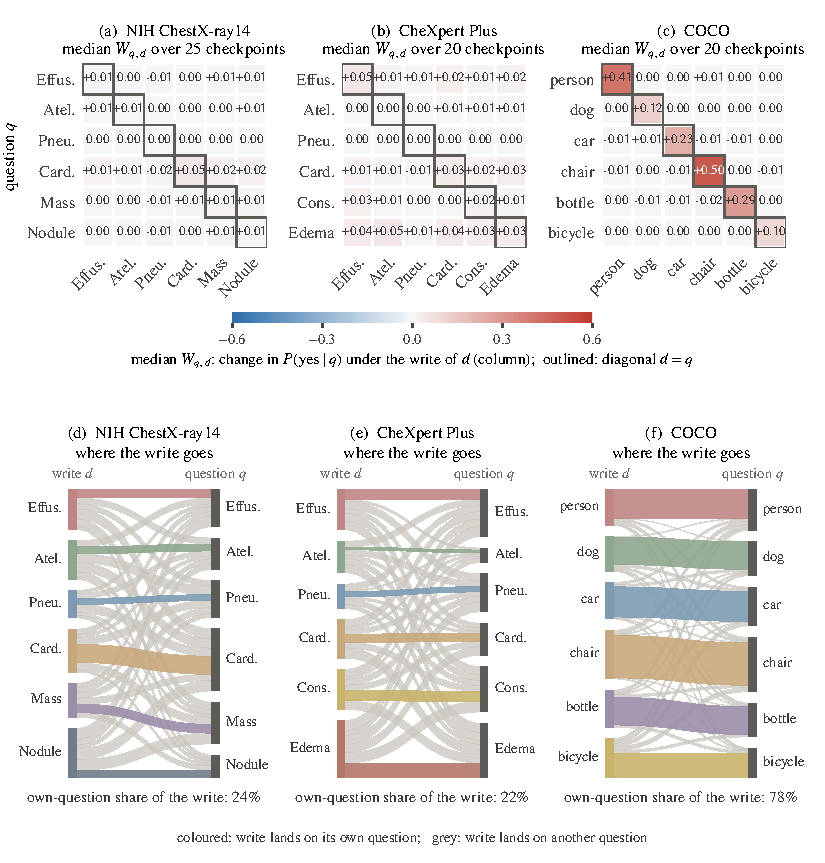
\includegraphics[width=\textwidth]{figures/figA1_write_structure.pdf}
    \caption{\textbf{Write structure across the grid.} (a--c) Cell-wise median of the write matrix $W_{q,d}$ over completed checkpoints on NIH ChestX-ray14, CheXpert Plus, and COCO. (d--f) Where the write goes: bands join each written direction $d$ (left) to the questions $q$ it moves (right), with width proportional to the mean over checkpoints of $\max(W_{q,d},0)$; coloured bands land on the writer's own question, grey bands on another. The share of the write that lands on its own question is printed under each panel.}
    \label{fig:cf-w-structure}
\end{figure}

\subsection{Per-image examples}
\label{app:cf-examples}

Figure~\ref{fig:cf-examples} shows grades on individual test images. For a chest example, the pool contains test rows where the finding is labelled present, the probe reads it (probability above $0.5$), and the clean answer is No. For a natural-image example, the pool contains rows where the probe reads the label correctly and the clean answer is No. We split each pool by whether the concept's own write or the strongest competing write raises the answer more. We show the row whose gap is closest to the median among rows where either write raises the answer by at least $0.2$. Each example's last line reports the number of pool rows with the same ordering, giving that example its own base rate.

\begin{figure}[p]
    \centering
    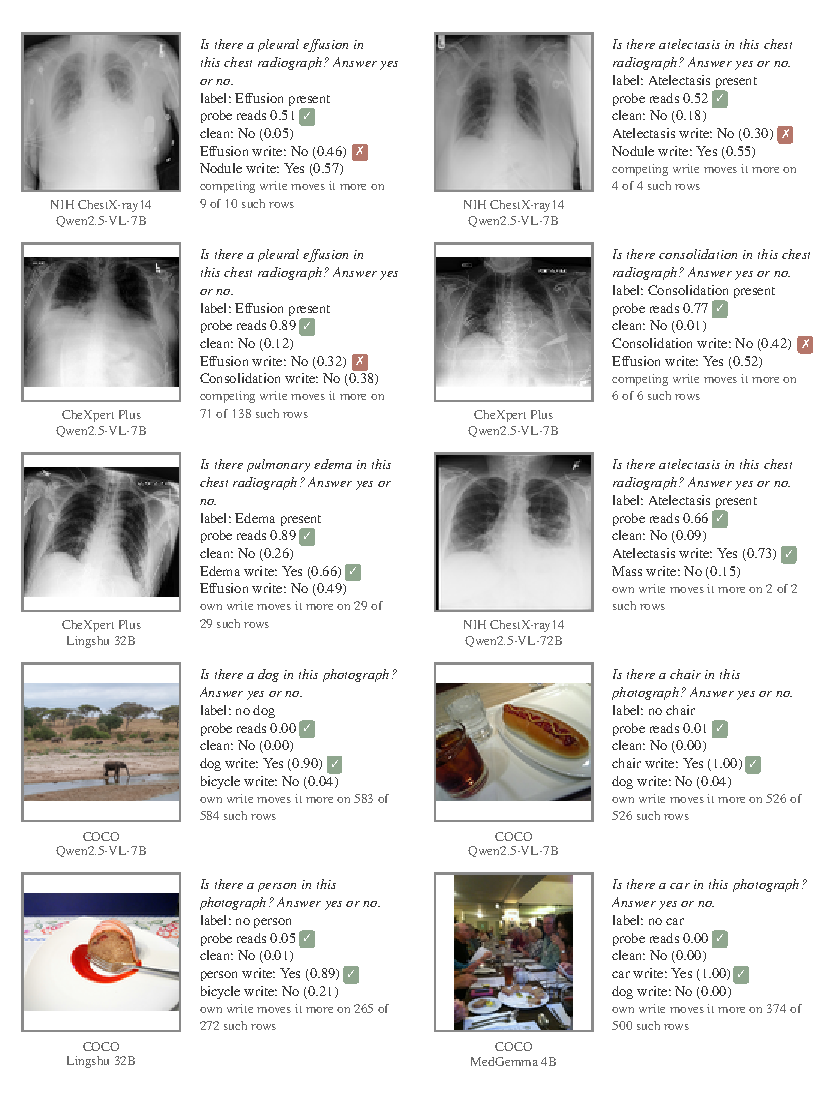
\includegraphics[width=\textwidth]{figures/figA2_examples.pdf}
    \caption{\textbf{Reading, answering, and writing on single images.} For each image: the question, the report label with the probe's reading, the clean answer, the answer under the concept's own write, and the answer under the strongest competing write, all at $\alpha=+0.25$ ($P(\mathrm{yes})$ in parentheses). A check on the write line means the concept's own direction raises its answer more than every competing direction on that image; a cross means a competitor raises it more. The first four chest examples are deficit cells of Qwen2.5-VL-7B; the next two are owned cells (Lingshu 32B Edema, Qwen2.5-VL-72B Atelectasis); the natural-image examples are owned cells of Qwen2.5-VL-7B, Lingshu 32B, and MedGemma 4B. The last line of each example counts the rows of its pool on which the same write wins.}
    \label{fig:cf-examples}
\end{figure}

\section{Seed study: registered protocol}
\label{app:seed}

The two-model study that motivated the evaluation registered the procedures below; Appendix~\ref{app:seed-results} reports its results.

\paragraph{Data and split.}
We use NIH ChestX-ray14 \citep{wang2017chestxray}, whose findings are mined from radiology reports. A deterministic hash of patient identity assigns rows to disjoint train, validation, and test partitions. The registered manifest contains 18,212 training images and 5,343 test images from 1,659 test patients. The three cells pair LLaVA-1.5-7B with Effusion and Edema, and Qwen2.5-VL-7B with Effusion. All reported uncertainty clusters by patient. Prompts appear in Appendix~\ref{app:protocol}.

\paragraph{Models and consumed loci.}
For LLaVA-1.5-7B \citep{liu2024improved} and Qwen2.5-VL-7B \citep{bai2025qwen25vl}, we use the final visual block consumed by the connector or merger. Writing $\alpha$ for the signed intervention dose, synthetic hook tests establish downstream-path membership, a bitwise $\alpha=0$ no-op, and changed downstream representations and logits at nonzero dose. Probe and intervention therefore share one consumed representation.

\paragraph{Controlled decodability.}
For image $i$, let $\hvec_{it}\in\R^D$ denote the $D$-dimensional representation of visual token $t$ at the consumed final block; mean pooling over tokens yields $\hvec_i$. A fixed seed-0 Gaussian matrix $R\in\R^{D\times512}$ projects every model to a common readout dimension; featurewise scale $\boldsymbol{s}$ is fitted on training rows only. We then fit logistic regression with $C=1$, maximum 2,000 iterations, and seed 0. Each of 20 control seeds maps the recurring input type (AP view indicator, sex indicator, and age decade, giving 39 strata) to a random label. Let $y$ be the real test labels and $r$ the fitted probe's continuous scores. For control seed $k\in\{0,\ldots,19\}$, $y_k^{\mathrm{ctrl}}$ denotes the random labels and $r_k^{\mathrm{ctrl}}$ the corresponding control probe scores. Selectivity compares their AUROCs:
\begin{equation}
S = \operatorname{AUROC}(y,r)-\frac{1}{20}\sum_{k=0}^{19}\operatorname{AUROC}(y_k^{\mathrm{ctrl}},r_k^{\mathrm{ctrl}}).
\label{eq:selectivity}
\end{equation}
We report the real AUROC, control distribution, and $S$ with 2,000 patient-cluster bootstrap resamples. A positive interval for $S$ means that the target is more readable than same-capacity nuisance-type label maps. It does not yet imply downstream use. Paired contrasts reuse identical ordered test rows and bootstrap draws.

\paragraph{Probe-normal intervention.}
Let $\boldsymbol\beta_c$ be the projected-space logistic coefficient for the positive class of concept $c$. We lift it to the consumed $D$-dimensional representation and normalize it exactly as
\begin{equation}
\hat\wvec_c = \frac{R\left(\boldsymbol\beta_c\oslash\max(\boldsymbol{s},10^{-8})\right)}{\left\lVert R\left(\boldsymbol\beta_c\oslash\max(\boldsymbol{s},10^{-8})\right)\right\rVert_2}.
\label{eq:lift}
\end{equation}
The positive-class coefficient fixes the direction's clinical pole. At every visual token $t$, the registered intervention is
\begin{equation}
\hvec'_{it}=\hvec_{it}+\alpha\lVert\hvec_{it}\rVert_2\hat\wvec_c.
\label{eq:intervention}
\end{equation}
Here the sign of $\alpha$ selects the positive or negative clinical pole, while $|\alpha|$ is the perturbation norm as a fraction of each token's activation norm. At the first answer position, $P(\mathrm{yes})=\sigma(\ell_{\mathrm{yes}}-\ell_{\mathrm{no}})$, where each log probability is the maximum over case and leading-space variants that tokenize to one token; the endpoint is its paired mean change from the common unsteered baseline. Original cells use concept doses $\{-1,-0.5,-0.25,-0.1,0,0.1,0.25,0.5,1\}$ on 200 held-out test images. Controls are evaluated at the six nonzero doses excluding $\pm0.1$: 20 isotropic random unit directions, one sham formed by a fixed coordinate permutation of $\hat\wvec_c$ and renormalization, and fixed alternative clinical probe normals. Every control receives the same signed dose on the same rows. Dose monotonicity over $[-0.5,0.5]$ is descriptive.

\paragraph{Original-cell decision rule.}
Let $\Delta_c(\alpha)$ be the target direction's paired mean probability change, and let $\mathcal A=\{-1,-0.5,-0.25,0.25,0.5,1\}$ be the six controlled doses. The primary effect is $\max_{\alpha\in\mathcal A}\operatorname{sign}(\alpha)\Delta_c(\alpha)$, attained at dose $\alpha^\star$. A cell clears the generic intervention gate when this selected effect exceeds the 95th percentile of the 20 random directions' mean probability changes at that same $\alpha^\star$, each multiplied by $\operatorname{sign}(\alpha^\star)$, and the maximum absolute sham effect over $\mathcal A$. The random directions are not separately maximized over doses. This asymmetric selection defines a registered reference gate, not a cross-dose-corrected 5\% test. The conjunction is fixed across the three cells. The independent supplement below instead evaluates a dose locked before observing its patients.

\paragraph{Direction-specificity supplement.}
The initial experiment prespecified the random and sham comparisons; its clinical-direction analysis was descriptive. The Nodule response motivated a separately registered supplement at the locked Qwen dose, $\alpha=+0.25$. We select one row by label-blind hash for each of 400 ChestX-ray14 test patients absent from the original 200-image intervention cohort. The semantic family contains all five non-target normals from the pre-existing Qwen direction bundle (Atelectasis, Pneumothorax, Cardiomegaly, Mass, and Nodule), rather than directions chosen from the supplement outcome. Each uses the same training rows, projection, scaling, classifier, lifting rule, and normalization as Effusion. Together with a common baseline, 20 random directions, and the sham, the grid produces 28 configurations and 11,200 per-image outcomes; exact row selection appears in Appendix~\ref{app:seed-results}.

Semantic ownership is a contrast on a direction--question response surface, not a property of a direction in isolation. Let $W_{q,d}$ denote the paired mean change in question $q$'s yes probability after intervening with direction $d$ at the locked dose. A large $W_{q,d}$ establishes that $d$ can write $q$'s answer; it does not establish that $d$ owns that answer. Within a fixed clinical family, the ownership contrast is
\begin{equation}
O_q=W_{q,q}-\max_{d\neq q}W_{q,d}.
\label{eq:margin}
\end{equation}
The registered supplement estimates the Effusion row of this surface, so the reported ownership contrast $O_{\mathrm{Effusion}}$ is Effusion minus its maximum alternative. The maximum is recomputed inside each of 5,000 patient-bootstrap draws. Thus $O_{\mathrm{Effusion}}>0$ means Effusion beats every member of the fixed clinical family, while $O_{\mathrm{Effusion}}<0$ means at least one alternative is stronger. Adding competitors can only maintain or decrease $O_q$: a positive advantage is conditional on the candidate family, whereas a negative counterexample does not require an exhaustive family. This operational ownership criterion measures relative advantage, not a necessary condition for a concept to participate in computation. Direction specificity requires a positive Effusion effect above random p95 and absolute sham, together with a one-sided 95\% lower bound for $O_{\mathrm{Effusion}}$ above zero.

\paragraph{Causal-ownership matrix.}
To test whether another clinical normal better matches the answer pathway, we prospectively cross six Qwen directions (Effusion, Atelectasis, Pneumothorax, Cardiomegaly, Mass, and Nodule) with their six matching questions on 400 new patients. Every question uses the same $\alpha=+0.25$, 119 random directions, and a sham. For question $q$, ownership requires the diagonal effect $W_{q,q}$ to exceed every other clinical direction, every random direction, and the absolute sham effect. A centered studentized max-$T$ bootstrap gives simultaneous 95\% lower bounds over all 30 clinical contrasts. The shared-alias family contains two statistics per direction: mean excess over the matching diagonals on its five off-diagonal questions and signed mean effect on those questions. These give 12 max-$T$ bounds; the effect must also exceed the random alias maximum and maximum absolute sham effect, detailed in Appendix~\ref{app:seed-results}.

For a family of $m$ statistics, let $\widehat C_j$ be statistic $j$'s estimate and $C^*_{bj}$ its value in joint patient-bootstrap draw $b$, with $B=5{,}000$ draws. Write $s_j=\operatorname{SD}_{b}(C^*_{bj})$ for the bootstrap standard deviation with denominator $B-1$, held fixed across draws, and $Q_{.95}$ for the empirical 95th percentile with linear interpolation. For $s_j>10^{-12}$, the centered standardized draw $Z_{bj}$, common critical value $c_{.95}$, and simultaneous lower bound $L_j$ are
\begin{equation}
Z_{bj}=\frac{C^*_{bj}-\widehat C_j}{s_j},\qquad
c_{.95}=Q_{.95}\!\left(\left\{\max_{1\leq j\leq m}Z_{bj}\right\}_{b=1}^{B}\right),\qquad
L_j=\widehat C_j-c_{.95}s_j.
\label{eq:max-t}
\end{equation}
Joint resampling preserves paired conditions; no standard error is re-estimated within a draw. Appendix~\ref{app:simultaneous-bounds} specifies the families, degenerate components, and the separate percentile intervals for target-minus-maximum margins.

\paragraph{Answer-encoding crossover.}
We next register a paired sensitivity study on 200 patients from the causal-ownership matrix cohort; the other 200 form a patient-disjoint capability-calibration set. This is not the earlier Effusion specificity cohort. Six questions cross the original yes/no prompt with A-present and B-present prompts, which exchange the finding-to-letter mapping. Each uses both $\alpha=\pm0.25$, six clinical directions, 20 random directions, and a sham. A question enters the primary endpoint only if both clean coded mappings have AUROC one-sided 95\% lower bounds above 0.5 and at least ten patients per class on calibration. At $\alpha=+0.25$, we compare squared mean effects in components that retain or reverse raw A-minus-B sign under the mapping exchange, using an unbiased estimator and 2,000 joint patient-bootstrap draws. Appendix~\ref{app:seed-results} defines the components and full control rule. Descriptive clinical competition uses the contrast in Equation~\ref{eq:margin}, replacing probability change with finding-present logit-margin change within each prompt.

\paragraph{Independent Mass confirmation.}
We prospectively test Mass on 200 patients absent from all preceding Qwen intervention cohorts, retaining the crossover's 200 calibration patients. Two question wordings (\textit{show}, \textit{is}) cross explicit yes/no, A-present, and B-present instructions; the original yes/no prompt is a seventh anchor. At $\alpha=+0.25$, each cell receives six clinical directions, 119 random directions, and a sham. The four coded cells share 20 clinical comparisons with simultaneous 95\% lower bounds. Confirmation requires positive bounds and Mass effects above every random effect and absolute sham, either across all four coded cells or both original-wording cells. Appendix~\ref{app:seed-results} specifies calibration and paired descriptive contrasts.


\section{Seed study: results}
\label{app:seed-results}

\begin{table}[t]
\centering
\scriptsize
\setlength{\tabcolsep}{4pt}
% Morandi tints for the cf-transfer tables (muted, low saturation); darker = larger value
\definecolor{cfSage1}{HTML}{EEF1EA}
\definecolor{cfSage2}{HTML}{D9E1D2}
\definecolor{cfSage3}{HTML}{C1CDB8}
\definecolor{cfSage4}{HTML}{A6B79C}
\definecolor{cfSlate1}{HTML}{ECEFF2}
\definecolor{cfSlate2}{HTML}{D3DAE2}
\definecolor{cfSlate3}{HTML}{B7C3D0}
\definecolor{cfSlate4}{HTML}{98A8B9}
\definecolor{cfTerra1}{HTML}{F5ECE9}
\definecolor{cfTerra2}{HTML}{E9D3CC}
\definecolor{cfTerra3}{HTML}{DAB5AA}
\definecolor{cfTerra4}{HTML}{C9968A}
\definecolor{cfOat1}{HTML}{F4EFE6}
\definecolor{cfOat2}{HTML}{E8DDC8}
\definecolor{cfGrey}{HTML}{E4E1DC}

\caption{\textbf{Seed replication: Qwen2.5-VL-7B on NIH ChestX-ray14, 600 new patients.} Per concept: probe selectivity $S$, clean-answer AUROC, concept write $W_{qq}$, the random-family 95th percentile and the absolute sham at the same dose, the rank of $W_{qq}$ among the 120 compared effects, the ownership contrast $O_q$ with its 95\% percentile interval, the strongest competing direction, and the max-$T$ verdict. Negative ownership is shaded terracotta.}
\label{tab:cf-seed}
\begin{tabular}{lrrrrrrrll}
\toprule
Concept & $S$ & AUROC & $W_{qq}$ & p95 & $|$sham$|$ & rank & $O_q$ [95\% CI] & Competitor & Verdict \\
\midrule
Effusion & 0.102 & 0.593 & +0.190 & 0.137 & 0.017 & 2/120 & \cellcolor{cfTerra2}-0.071 [-0.080, -0.062] & Nodule & competitor \\
Atelectasis & 0.062 & 0.566 & +0.101 & 0.297 & 0.096 & 55/120 & \cellcolor{cfTerra3}-0.226 [-0.233, -0.219] & Nodule & competitor \\
Pneumothorax & 0.152 & 0.508 & +0.089 & 0.320 & 0.113 & 52/120 & \cellcolor{cfTerra3}-0.102 [-0.108, -0.096] & Effusion & competitor \\
Cardiomegaly & 0.205 & 0.742 & +0.085 & 0.311 & 0.158 & 33/120 & \cellcolor{cfTerra3}-0.219 [-0.227, -0.211] & Atelectasis & competitor \\
Mass & 0.021 & 0.678 & +0.359 & 0.372 & 0.092 & 10/120 & \cellcolor{cfTerra3}-0.169 [-0.178, -0.160] & Effusion & competitor \\
Nodule & -0.041 & 0.642 & +0.118 & 0.158 & 0.055 & 15/120 & \cellcolor{cfTerra2}-0.072 [-0.081, -0.063] & Effusion & competitor \\
\bottomrule
\end{tabular}
\end{table}


\subsection{A non-generic write effect reproduces}
\label{sec:qwen-replication}

The first finding starts with a successful intervention: Qwen Effusion reproduces beyond random and sham controls before clinical alternatives change its attribution.

Controlled decodability is evaluated at the final visual block each connector consumes: the penultimate CLIP encoder layer for LLaVA and the last of Qwen's 32 visual blocks. Intervals are 95\% patient-cluster bootstrap intervals over 2,000 draws; the control AUROC is the mean over the 20 recurring-type random-label maps, with its 5th--95th percentile spread in parentheses.

Qwen Effusion first satisfies the reader test. Its probe reaches AUROC \cfSeedDecQwenEffAuroc{} $[\cfSeedDecQwenEffAurocLo,\cfSeedDecQwenEffAurocHi]$ against a control AUROC of \cfSeedDecQwenEffCtrl{} (\cfSeedDecQwenEffCtrlLo--\cfSeedDecQwenEffCtrlHi), a controlled selectivity of \cfSeedDecQwenEffSel{} (95\% CI $[\cfSeedDecQwenEffSelLo,\cfSeedDecQwenEffSelHi]$). LLaVA-1.5-7B reads both of its concepts at its consumed block: Effusion at AUROC \cfSeedDecLlavaEffAuroc{} $[\cfSeedDecLlavaEffAurocLo,\cfSeedDecLlavaEffAurocHi]$ with selectivity \cfSeedDecLlavaEffSel{} $[\cfSeedDecLlavaEffSelLo,\cfSeedDecLlavaEffSelHi]$, and Edema at AUROC \cfSeedDecLlavaEdemaAuroc{} $[\cfSeedDecLlavaEdemaAurocLo,\cfSeedDecLlavaEdemaAurocHi]$ with selectivity \cfSeedDecLlavaEdemaSel{} $[\cfSeedDecLlavaEdemaSelLo,\cfSeedDecLlavaEdemaSelHi]$, against a control AUROC of \cfSeedDecLlavaEffCtrl{} (\cfSeedDecLlavaEffCtrlLo--\cfSeedDecLlavaEffCtrlHi). Original-cohort intervention outcomes maximize the concept-consistent effect over six fixed nonzero doses. Qwen makes a strong write-direction case in the original 200-image cohort: the maximum concept-consistent change is 0.2343 at $\alpha=+0.25$, above the random-direction 95th percentile of 0.0963 and the maximum absolute sham effect of 0.0852.

The response at the locked dose $\alpha=+0.25$ reproduces on the patient-disjoint 400-patient cohort. Effusion changes mean $P(\mathrm{yes})$ by 0.1945, again above the random-direction 95th percentile of 0.0878 and absolute sham effect of 0.0157. None of these patients appears in the original intervention cohort, and the dose was not reselected, supporting a large and reproducible non-generic effect within ChestX-ray14.


\subsection{Semantic competition changes attribution, not efficacy}
\label{sec:specificity-results}

The fixed clinical family provides a harder identification test than non-semantic controls. Nodule changes the Effusion answer by 0.2519 and realizes the point-estimate maximum among the five alternatives. The Effusion ownership contrast $O_{\mathrm{Effusion}}$ is $-0.0573$. The registered fixed-family endpoint recomputes the maximum inside each of 5,000 patient-bootstrap draws, giving a two-sided 95\% CI of $[-0.0694,-0.0450]$ and a one-sided 95\% lower bound of $-0.0678$. The entire interval is below zero. Descriptively, all five alternative clinical normals move the Effusion endpoint in the same positive direction; Effusion exceeds four by 0.1172--0.1778, while Nodule alone has a larger point estimate. This shared-sign pattern motivates an answer-sensitive-alias hypothesis but cannot distinguish it from question-specific ownership.

Qwen Effusion therefore remains a reproducible direction that changes the answer beyond random and sham perturbations, while its specific semantic attribution fails. The familywise endpoint establishes that at least one fixed clinical alternative is stronger; Nodule is the point-estimate maximizer, not a separately familywise-identified semantic owner.

\subsection{Wording changes clinical competition within the answer interface}
\label{sec:encoding-results}

The second finding concerns the conditions of clinical competition. The Qwen ownership pattern persists in logit coordinates, so we test whether changing the answer interface changes a direction's relative advantage.

In the registered crossover, Atelectasis, Pneumothorax, Mass, and Nodule pass independent capability calibration. On these four questions, mapping-even minus mapping-odd response energy is $-2.1786$ (95\% CI $[-2.4061,-1.9810]$): effects are larger in the component that reverses raw A-minus-B sign when the finding-to-letter mapping is exchanged. Yet all 20 random directions and the sham are also mapping-odd dominant. Aggregate mapping response therefore does not distinguish the clinical normals from generic perturbations.

The crossover identifies Mass as a prompt-conditioned candidate: its clinical margin changes from $-0.7181$ under the original yes/no prompt to $0.2825$ and $0.2900$ under A-present and B-present, respectively (Table~\ref{tab:seed-mass}, top). A-present assigns A to presence and B to absence; B-present reverses those assignments. Both coded effects exceed the discovery study's 20 random directions and sham. The top rows of Table~\ref{tab:seed-mass} carry pointwise 95\% intervals. Because wording and instructions also change, we test them separately on independent patients.

\begin{table}[H]
\centering
\scriptsize
\setlength{\tabcolsep}{5pt}
\caption{\textbf{Mass clinical competition across prompts.} Clinical margin per prompt: the Mass effect minus the largest of the five other clinical effects, in finding-present logit units. Top, the discovery crossover; bottom, the registered confirmation on new patients.}
\label{tab:seed-mass}
\begin{tabular}{lrrrrr}
\toprule
Prompt & Clinical margin & 95\% CI & Mass effect & Random max & $|$Sham$|$ \\
\midrule
Standard yes/no & $-0.7181$ & $[-0.7956,-0.6412]$ & 2.8625 & 3.0412 & 0.5869 \\
A-present & $0.2825$ & $[0.2269,0.3406]$ & 1.6125 & 1.1650 & 0.7550 \\
B-present & $0.2900$ & $[0.2300,0.3506]$ & 1.7469 & 1.2581 & 1.1475 \\
\midrule
Condition & Clinical margin & Minimum LCB & Mass effect & Random max & \\
\midrule
\textit{show}/A-present & 0.2525 & 0.1675 & 1.7019 & 2.2100 & \\
\textit{show}/B-present & 0.2338 & 0.1462 & 1.8188 & 2.2169 & \\
\textit{is}/A-present & $-0.1087$ & $-0.1751$ & 1.9225 & 2.4750 & \\
\textit{is}/B-present & $-0.2006$ & $-0.2686$ & 2.0019 & 2.4944 & \\
\bottomrule
\end{tabular}
\end{table}


The bottom of Table~\ref{tab:seed-mass} reports the registered confirmation on 200 new patients. Clinical margins subtract the largest of five alternative clinical effects in finding-present logit units. Minimum LCB is the smallest simultaneous lower bound among a cell's five contrasts, from the joint 20-comparison family. All seven prompt cells pass separate capability calibration.

The clinical advantage reproduces under both \textit{show} coded prompts, but the Mass effects remain below the maxima of 119 random directions, with reference ranks of 3/120. These 119 directions form a fixed reference family: each rank places Mass third among the 120 compared effects. This finite descriptive ranking is not a $p$-value, and failure to exceed this family's maximum does not establish nonspecificity across arbitrary direction distributions or reference-family sizes. Under \textit{is}, both clinical margins are negative. Neither the cross-wording nor original-wording specificity conjunction is met.

Explicit \textit{show} yes/no also has a positive clinical margin, 0.2369; its paired differences from A-present and B-present span zero. Within each response instruction, changing \textit{show} to \textit{is} reduces the clinical margin. These paired wording contrasts are descriptive. They support wording-conditioned clinical competition, rather than an advantage attributable to answer letters alone. Mass steering increases Brier error in every cell, while all AUROC-change intervals span zero.

\FloatBarrier

\section{Prompts, Scores, and Notation}
\label{app:protocol}

\subsection{A common question and answer endpoint}

At the first answer position, let $\ell_{\mathrm{yes}}$ and
$\ell_{\mathrm{no}}$ denote the maximum log probabilities among the valid
single-token case and leading-space variants of each answer.  The registered
score is $P(\mathrm{yes})=\sigma(\ell_{\mathrm{yes}}-\ell_{\mathrm{no}})$,
where $\sigma$ is the logistic sigmoid. The original Edema cell uses ``pulmonary
edema,'' and the closure experiment uses ``consolidation'' in the same
template. Taking the best valid token variant for each answer makes the
endpoint insensitive to which listed capitalization or leading-space form
receives the highest score. This endpoint measures the relative support for
yes versus no at the first answer position; it does not measure the accuracy
of a generated clinical report.


The shared interface makes the question--direction grid interpretable:
changing a clinical direction does not change the question being scored.
Differences across columns still reflect different clinical questions, so
the ownership test compares directions within each column before drawing
a conclusion about the named concept.

\subsection{Reading the intervention notation}

Table~\ref{tab:notation} collects the notation introduced in the article.
The distinction between question $q$ and direction $d$ is central: a large
$W_{q,d}$ shows that a direction moves an answer, while $O_q$ asks whether
the direction bearing that answer's clinical name moves it more than its
competitors. A positive ownership margin alone is not the full confirmation
rule; the uncertainty and non-semantic control comparisons must also pass.
Keeping these roles separate allows the following analyses to distinguish
readability, intervention strength, and semantic attribution.

\begin{table}[H]
\centering
\caption{Notation used in the manuscript.}
\label{tab:notation}
\resizebox{\ifdim\width>\linewidth\linewidth\else\width\fi}{!}{%
\begin{tabular}{ll}
\toprule
Symbol & Definition \\
\midrule
$q,d,c$ & Clinical question, steering direction, and probe concept, respectively. \\
$\hvec_{it}$ & Consumed visual representation for image $i$ and visual token $t$. \\
$R,\boldsymbol{s}$ & Fixed Gaussian projection and train-fitted featurewise scale. \\
$\hat\wvec_c$ & Unit probe-normal direction for concept $c$ after lifting to the consumed representation. \\
$\alpha$ & Signed intervention dose; $|\alpha|$ is the perturbation norm relative to each token norm. \\
$W_{q,d}$ & Paired mean change in question $q$'s $P(\mathrm{yes})$ under direction $d$. \\
$O_q$ & Ownership margin $W_{q,q}-\max_{d\neq q}W_{q,d}$; positive values favor the named direction. \\
$S$ & Real-label AUROC minus the mean AUROC of the 20 nuisance-type control tasks. \\
$\gamma_i$ & Positive-minus-negative paired representation displacement along the Consolidation normal. \\
\bottomrule
\end{tabular}
}
\end{table}

The notation separates three levels of evidence: $S$ describes label
availability, $W_{q,d}$ describes an intervention effect, and $O_q$ compares
the named direction with clinical alternatives. The remaining appendix
follows this progression while keeping the evaluation cohorts explicit.

\FloatBarrier


\section{Joint bootstrap and simultaneous lower bounds}
\label{app:simultaneous-bounds}

Equation~\ref{eq:max-t} uses the standard deviation across bootstrap
estimates as a fixed scale for each statistic. With $\overline C^*_j$
denoting their mean, that scale is
\begin{equation}
s_j=\left[\frac{1}{B-1}\sum_{b=1}^{B}
       (C^*_{bj}-\overline C^*_j)^2\right]^{1/2}.
\label{eq:bootstrap-scale}
\end{equation}
The standardized deviations are centered on the observed $\widehat C_j$,
not on $\overline C^*_j$. For a component with $s_j\leq10^{-12}$,
all its $Z_{bj}$ values are set to zero. If every component satisfies
that threshold, the critical value is zero. Otherwise, each draw's
maximum includes these zero components, and its empirical 95th percentile
uses linear interpolation. All 5,000 draws are retained. The final
subtraction $L_j=\widehat C_j-c_{.95}s_j$ still uses the actual $s_j$,
including for thresholded components.

For the ownership matrix, we resample 400 patients with replacement using seed 20260904. Each draw uses the same patient indices for every question and intervention, preserving all paired baseline differences. The clinical family comprises the 30 fixed contrasts $W_{q,q}-W_{q,d}$ for the six questions and their five alternatives. Each question's simultaneous ownership lower bound is the minimum of its five contrast bounds. Simultaneous upper bounds use the same critical value with the sign of every contrast reversed. A question has a stronger competitor if any upper bound is below zero. A question is unresolved if it has neither a positive minimum lower bound nor a negative upper bound. The shared-alias calculation uses a separate 12-statistic family: for each of six directions, its mean off-diagonal effect and its mean excess over the five corresponding matched-direction effects. The Mass confirmation applies the same construction to 200 independently selected patients, with seed 20260910 and a separate family of 20 Mass-minus-alternative contrasts across four coded prompt conditions.

Direct target-minus-maximum intervals summarise a different bootstrap quantity. For each draw, we recompute the largest competing mean and subtract it from the target mean. The displayed two-sided percentile intervals use the 2.5th and 97.5th percentiles of these margins. The earlier Effusion specificity supplement uses their 5th percentile as its one-sided lower bound. These intervals are distinct from the simultaneous bounds on the fixed linear contrasts in Equation~\ref{eq:max-t}.

The campaign applies the same construction to every block, using 600 test rows and 2{,}000 shared bootstrap draws of rows (seed 2026090601). The 30 contrasts $W_{q,q}-W_{q,d}$ receive simultaneous 95\% bounds from the centred studentised max-$T$ bootstrap. $O_q$ receives a direct percentile interval with the maximum recomputed in every draw. The logit-scale check in Table~\ref{tab:cf-scale} applies the same rules to margin-scale deltas.
\section{Reproducibility specification}
\label{app:repro}

This appendix documents the hook paths, consumed-token mask, projection and probe, control constructions, cohort roles, and protocol record. Every statement below comes from the released adapters (\texttt{src/cftransfer/adapters/}), the registered protocol file, and the per-block artifacts.

\subsection{Consumed loci per family}
\label{app:repro-loci}

Table~\ref{tab:cf-loci} gives the primary and connector locus module paths exactly as the adapters name them, together with the rule for identifying the consumed final block. Each adapter resolves the block index at load time from the loaded checkpoint's own configuration. Each block's preflight file records the resolved path, hidden dimension, consumer, and any branch that bypasses the locus. Table~\ref{tab:cf-models} gives the consumed-token count per image at the primary locus for every checkpoint.

\begin{table}[h]
\centering
\scriptsize
\setlength{\tabcolsep}{4pt}
\caption{\textbf{Hook paths per checkpoint family.} Module paths as the adapters name them under the loaded model. $n$ is the length of the block list of that checkpoint's tower; the adapter resolves it at load time and the block's preflight file records the resolved path.}
\label{tab:cf-loci}
\begin{tabular}{>{\raggedright\arraybackslash}p{0.15\textwidth}>{\raggedright\arraybackslash}p{0.25\textwidth}>{\raggedright\arraybackslash}p{0.20\textwidth}>{\raggedright\arraybackslash}p{0.28\textwidth}}
\toprule
Family (adapter) & Primary locus & Connector locus & Consumed final block identified by \\
\midrule
Qwen2.5-VL, Qwen3-VL, Lingshu (\texttt{qwen}) & \texttt{model.visual.blocks.}$(n{-}1)$ & \texttt{model.visual.merger} & The merger reads the last entry of \texttt{model.visual.blocks}: $n=32$ for Qwen2.5-VL and Lingshu, $24$ for Qwen3-VL 4B, $27$ for Qwen3-VL 8B and 32B. The Qwen3-VL DeepStack mergers read earlier blocks and are not hooked. \\
\addlinespace[2pt]
Gemma~3, MedGemma (\texttt{gemma}) & \texttt{model.vision\_tower.}\allowbreak\texttt{encoder.layers.26} & \texttt{model.}\allowbreak\texttt{multi\_modal\_projector} & The projector reads the last SigLIP encoder layer, 26 of 27. \texttt{post\_layernorm} sits between that layer and the projector. \\
\addlinespace[2pt]
InternVL3.5 (\texttt{internvl}) & \texttt{model.vision\_tower.}\allowbreak\texttt{encoder.layer.}$(n{-}1)$ & \texttt{model.}\allowbreak\texttt{multi\_modal\_projector} & The projector reads the last InternViT encoder layer, $n=24$ at 8B and 14B and $n=45$ at 38B, after \texttt{vision\_tower.layernorm}, which is an identity under the shipped \texttt{use\_mean\_pooling} configuration. \\
\addlinespace[2pt]
LLaVA-1.5, LLaVA-Med (\texttt{llava}) & \texttt{model.vision\_tower.}\allowbreak\texttt{encoder.layers.22} & \texttt{model.}\allowbreak\texttt{multi\_modal\_projector} & The checkpoint's \texttt{vision\_feature\_layer} is $-2$, so the projector reads CLIP encoder layer 22 of 24 and the final layer is computed and discarded. \\
\addlinespace[2pt]
Llama~3.2 Vision (\texttt{mllama}) & \texttt{model.vision\_model.}\allowbreak\texttt{global\_transformer.layers.7} & \texttt{model.}\allowbreak\texttt{multi\_modal\_projector} & The projector input concatenates the last global-transformer layer, 7 of 8, with the outputs of local layers 3, 7, 15, 23 and 30; those five bypass the primary locus. \\
\bottomrule
\end{tabular}
\end{table}
\FloatBarrier

\subsection{The consumed-token mask}
\label{app:repro-mask}

The write of Equation~\ref{eq:intervention} changes only the entries of the hooked tensor corresponding to token positions the consumer reads at that locus. The adapter derives these positions for each batch from the processor's own outputs. Two tensor shapes occur. The Qwen family passes the merger a flat $(N,D)$ tensor in which every image occupies one contiguous slice. The adapter computes the slice bounds from \texttt{image\_grid\_thw} (the connector slice is a quarter of the length, one merged token per $2\times2$ patch group). Every other family passes the consumer a batched $(B,T,D)$ tensor. The adapter supplies one boolean mask per batch element:

\begin{itemize}[leftmargin=*,itemsep=1pt,topsep=2pt]
\item Gemma~3 and MedGemma: all 4{,}096 patch rows; the tower produces no CLS row. The mask length is checked against the count of \texttt{<image\_soft\_token>} placeholders in the language-model input.
\item InternVL3.5: index 0 is the CLS row, which the consumer drops, so it is excluded; the remaining rows of the single $448\times448$ tile are written. The mask length is checked against the count of \texttt{<IMG\_CONTEXT>} placeholders.
\item LLaVA-1.5 and LLaVA-Med: index 0 is the CLS row, which the checkpoint's \texttt{vision\_}\allowbreak\texttt{feature\_}\allowbreak\texttt{select\_}\allowbreak\texttt{strategy} drops under its \texttt{default} setting, so it is excluded; rows 1 to 576 are written.
\item Llama~3.2 Vision: the 1{,}601 rows (CLS and 1{,}600 patches) of the one real $560\times560$ tile. The seven zero-padding rows of each tile and the three padding tiles are excluded, and the mask is checked against \texttt{aspect\_ratio\_mask} and the last position of \texttt{cross\_attention\_mask}.
\end{itemize}

The hook raises an error rather than falling back when a flat layout does not exactly cover the hooked tensor, a mask length differs from the token-axis length, a batch element has no consumed token, or the hooked module fires more than once in one forward pass.

Preflight check (C) verifies the mask. It captures the locus tensor on a clean pass and a pass steered at $\alpha=+0.25$ along the first concept direction. It reports the largest absolute difference outside the mask and the largest absolute changes in the consumer's output and answer logits. Across all \cfBlocks{} blocks, the change outside the consumed tokens is $0$ at both loci, while both the consumer's output and the answer logits change. The same files record a bitwise-identical repeated clean pass (check A) and a bitwise-identical $\alpha=0$ pass (check B) for every block.

\subsection{Projection, lift, scaler, and probe}
\label{app:repro-probe}

The projection $R\in\R^{D\times512}$ is one draw of \texttt{PCG64(0).standard\_normal((D,512))} divided by $\sqrt{512}$ and stored in float32. Its entries are independent $\mathcal{N}(0,1/512)$ variates. The seed is $0$ for every checkpoint, dataset, and locus; $D$ is the family's hidden dimension. We neither normalise nor orthogonalise the columns of $R$. We normalise the lifted direction of Equation~\ref{eq:lift} once, in model space, to unit $\ell_2$ norm. The Gram matrix $R^{\top}R/D$ has full rank 512 in every one of the \cfAltdirdBlocks{} blocks that carry the displacement module, with condition number \cfAltdirdCondMin{}--\cfAltdirdCondMax{}. Table~\ref{tab:cf-altdird} reports its eigenvalue range.

The token-mean read vector $\hvec_i$ yields projected features $R^{\top}\hvec_i$. A \texttt{StandardScaler} fitted only on training rows supplies the featurewise scale $\boldsymbol s$ and mean. Every row is standardised as $(R^{\top}\hvec-\boldsymbol\mu)\oslash\max(\boldsymbol s,10^{-8})$. Each concept probe uses \texttt{LogisticRegression} with $C=1$, \texttt{solver="lbfgs"}, \texttt{max\_iter=2000}, \texttt{class\_weight=None}, and \texttt{random\_state=0}, fitted on training rows with a known label for that concept. The positive-class coefficient fixes the clinical pole of the direction. For each of the two refit seeds, we resample training units with replacement, retain every row of each sampled unit at that unit's multiplicity, and refit the scaler and six probes using the same projection. The random family, shams, and control probes remain at seed 0.

\subsection{Control constructions}
\label{app:repro-controls}

\paragraph{Random directions.} We draw one $119\times D$ standard-normal matrix with \texttt{PCG64(0)} and normalise each row to unit $\ell_2$ norm. The same 119 directions serve every question in the block.

\paragraph{Coordinate-permutation sham.} Immediately after the random draw, the same generator produces one permutation of $\{0,\dots,D{-}1\}$ per concept in protocol concept order. Concept $c$'s sham is $\hat\wvec_c$ with its coordinates rearranged by concept $c$'s own permutation. The sham preserves the direction's coordinate multiset and unit norm. Each question is written with its own sham.

\paragraph{Matched random-label probes.} Each row has a type identifier: view $\times$ sex $\times$ age decade on the chest sets, and aspect-ratio $\times$ area buckets on COCO. For control seed $k\in\{0,\dots,19\}$, we traverse the sorted type names and draw one label per type from \texttt{PCG64($k$).integers(0,2)}; if all types receive the same label, we flip the first entry. Every row of a type receives that type's label. We fit each control probe on the same training rows and known-label subset, with the same hyperparameters as the concept probe, giving it the concept probe's capacity and nuisance structure. A block fits control probes when its training rows span at least eight types. Selectivity is Equation~\ref{eq:selectivity}. Its bootstrap over calibration units keeps a draw when the real AUROC is finite and at least ten of the twenty control AUROCs are finite. We grade a cell for readability when at least 1{,}900 of the 2{,}000 draws are kept.

\subsection{Cohort roles}
\label{app:repro-cohorts}

Table~\ref{tab:cf-roles} lists each role's size and use. The roles are disjoint by patient on the chest sets and by image on COCO. We use the calibration role only to determine readability and answer capability. We fit no probe and score no write on it. The test role carries every write.

\begin{table}[h]
\centering
\scriptsize
\setlength{\tabcolsep}{5pt}
\caption{\textbf{Cohort roles.} Rows per role with independent units in parentheses, and the role's use. The units are patients on the chest sets and images on COCO.}
\label{tab:cf-roles}
\begin{tabular}{llll>{\raggedright\arraybackslash}p{0.42\textwidth}}
\toprule
Role & NIH ChestX-ray14 & CheXpert Plus & COCO & Use \\
\midrule
train & 18{,}212 (5{,}783) & 20{,}000 (20{,}000) & 20{,}000 (20{,}000) & Scaler, six concept probes, twenty control probes, the two nuisance probes of the chest sets, and the answer-direction ridge. No row of this role is scored. \\
preflight & 16 (16) & 16 (16) & 16 (16) & The seven acceptance gates, at both loci. \\
calibration & 400 (400) & 400 (400) & 400 (400) & Clean pass at $\alpha=0$: probe readability and answer capability. \\
test & 600 (600) & 600 (600) & 600 (600) & Every write matrix, dose, refit, template, locus, and addendum module. \\
valid & -- & \cfValidRows{} (\cfValidRows{}) & -- & The regrade on radiologist consensus labels (Table~\ref{tab:cf-valid}). \\
\bottomrule
\end{tabular}
\end{table}
\FloatBarrier

\subsection{Protocol record and amendments}
\label{app:repro-protocol}

Each block writes a run record containing the protocol identifier \texttt{cf-transfer-v1}, the run identifier \texttt{cf-transfer-v1:<checkpoint>:<dataset>:mayo}, the evaluation-code commit that produced the block, the pinned checkpoint and processor revisions, the library versions, the dtypes, and the resolved processing settings, including the rendered chat template. All \cfBlocks{} blocks carry the protocol identifier \texttt{cf-transfer-v1}. The protocol file registers its own code reference commit \texttt{763072d3}.

Table~\ref{tab:cf-amendments} lists additions to the protocol file after the first wave and the date of each addition. The six planned modules and the connector calibration derived from them carry no amendment date. The robustness tables in Appendix~\ref{app:cf-robustness} identify the blocks that carry each amendment module.

\begin{table}[h]
\centering
\scriptsize
\setlength{\tabcolsep}{5pt}
\caption{\textbf{Protocol amendments.} Each entry is dated by the \texttt{added} field of the registered protocol file; the first two carry the identifiers of the execution log.}
\label{tab:cf-amendments}
\begin{tabular}{ll>{\raggedright\arraybackslash}p{0.58\textwidth}}
\toprule
Amendment & Date & Change \\
\midrule
A1 & 2026-09-14 & Per-block primary template: the single-template modules score the first eligible template in the order (IY, IB), so a checkpoint whose yes/no template fails the image-free mapping gate is graded on its B-positive template. Llama~3.2 Vision 11B re-ran on all three datasets. \\
A2 & 2026-09-14 & CheXpert gains DOSE, REFIT, LOCUS, LOCUS\_CALIBRATION and PROMPT, with Effusion and Edema as its PROMPT concepts. \\
ALTDIR (A3) & 2026-09-14 & Four alternative direction constructions per concept: difference of class means, Haufe pattern, orthogonalised normal, and residualised normal. \\
EXTCOMP & 2026-09-14 & Extra clinical directions for every additional dataset label with at least 100 known positives and negatives, added to the competitor family. \\
TOKENW & 2026-09-14 & Softmax-weighted and top-quarter token weights for the six logistic directions. \\
PRECISION & 2026-09-14 & The write grid rescored with fp32 weights and forward pass, and in bf16 at batch size one. \\
ANSDIR & 2026-09-14 & The answer direction: a ridge regression of the clean answer margin on the same projected, train-scaled features. \\
ALTDIRD & 2026-09-15 & The difference-of-means and pattern vectors lifted as displacements through the minimum-norm preimage. \\
ATTR & 2026-09-15 & Three non-clinical attribute directions written with the six clinical directions as one nine-direction family. \\
ANSDIRT & 2026-09-15 & The IY-fitted answer directions written under the five held-out templates. \\
VALID & 2026-09-15 & The write grid regraded on the CheXpert validation split with radiologist consensus labels. \\
\bottomrule
\end{tabular}
\end{table}

\FloatBarrier

\end{document}
